\documentclass{article}

\usepackage[top=3cm, bottom=3cm, left=3cm,right=3cm]{geometry}
\usepackage[colorinlistoftodos]{todonotes}
\usepackage{graphicx}
\usepackage{amssymb}
\usepackage{amsmath}
% \usepackage{gensymb}
\usepackage{todonotes}
\usepackage{pdflscape}
\usepackage{caption}
\usepackage{subcaption}
\usepackage[sort,round]{natbib}
\usepackage[T1]{fontenc}
\usepackage[utf8]{inputenc}
\usepackage{authblk}
% \usepackage{gensymb}
\usepackage{pdfpages}
\usepackage{setspace}
\usepackage{booktabs}
\usepackage{longtable}
\usepackage{float}
\usepackage{tikz}
\usepackage{tcolorbox}
\usepackage[colorlinks=true,citecolor=blue, linkcolor=blue]{hyperref}

\renewcommand\Affilfont{\itshape\footnotesize}
\def\ci{\perp\!\!\!\perp}

\renewcommand\Affilfont{\itshape\footnotesize}
\linespread{1.5}

\title{Technical Report \\Data Integration Model for Exposures (DIMEX-UK)}

\author[1]{Matthew L. Thomas}
\author[1]{Gavin Shaddick}
\author[2]{David Topping}
\author[3]{Karyn Morrissey}
\author[2]{Thomas J. Brannan}
\author[4]{Mike Diessner}
\author[5]{Ruth C. E. Bowyer}
\author[6]{Stefan Siegert}
\author[2]{Hugh Coe}
\author[7]{James Evans}
\author[8]{Fernando Benitez-Paez}
\author[9]{Jim Zidek}



\affil[1]{Department of Mathematics, University of Exeter \& Met Office - University of Exeter Joint Centre for Excellence in Environmental Intelligence, Exeter, United Kingdom.}
\affil[2]{Department of Earth and Environmental Sciences, University of Manchester, Manchester, United Kingdom}
\affil[3]{Sustainability Division, Department of Technology, Management and Economics, Technical University of Denmark, Lyngby, Denmark.}
\affil[4]{School of Computing, Newcastle University, Newcastle, United Kingdom.}
\affil[5]{Alan Turing Institute, London, United Kingdom \& Department of Twin Research and Genetic Epidemiology, King's College London, London, United Kingdom.}
\affil[6]{Department of Mathematics, University of Exeter,  Exeter, United Kingdom.}
\affil[7]{Department of Geography, School of Environment, Education and Development, University of Manchester, Manchester, United Kingdom.}
\affil[8]{Alan Turing Institute, London, United Kingdom.}
\affil[9]{Department of Statistics, University of British Columbia, Canada.}

\date{}

%%%%%%%%%%%%%%%%%%%%%%%%%%%%%%%%%%%%%%%%%%%%%%%%%%%%%%%%%%%%%%%%%%
%%%%%%%%%%%%%%%%%%%%%%%%%%%%%%%%%%%%%%%%%%%%%%%%%%%%%%%%%%%%%%%%%%
%%%%%%%%%%%%%%%%%%%%%%%%%%%%%%%%%%%%%%%%%%%%%%%%%%%%%%%%%%%%%%%%%%

\begin{document}
% Preamble
\maketitle
\newpage 

%%%%%%%%%%%%%%%%%%%%%%%%%%%%%%%%%%%%%%%%%%%%%%%%%%%%%%%%%%%%%%%%%%
%%%%%%%%%%%%%%%%%%%%%%%%%%%%%%%%%%%%%%%%%%%%%%%%%%%%%%%%%%%%%%%%%%
%%%%%%%%%%%%%%%%%%%%%%%%%%%%%%%%%%%%%%%%%%%%%%%%%%%%%%%%%%%%%%%%%%

\section*{Executive Summary}

%%%%%%%%%%%%%%%%%%%%%%%%%%%%%%%%%%%%%%%%%%%%%%%%%%%%%%%%%%%%%%%%%%
%%%%%%%%%%%%%%%%%%%%%%%%%%%%%%%%%%%%%%%%%%%%%%%%%%%%%%%%%%%%%%%%%%
%%%%%%%%%%%%%%%%%%%%%%%%%%%%%%%%%%%%%%%%%%%%%%%%%%%%%%%%%%%%%%%%%%

Air pollution poses significant threats to human health and in the UK, poor air quality is the largest environmental risk to public health. The majority of the research related to the health effects of air pollution has been at the population level, based on measured and modelled concentrations of ambient pollution at people's residential address. However, there is a need to increase our understanding of the (personal) exposures actually experienced by individuals as they move between different locations, such as the home, workplace or transport, throughout the day. \\

\noindent The Data Integration Model for Exposures (DIMEX-UK) integrates data on daily travel patterns and activities with measurements and models of air pollution using agent-based modelling to simulate the daily exposures of different population groups. Exposure profiles are simulated for a virtual population of individuals that reflect the demographic, socioeconomic and daily movement patterns of real-life individuals within an area. The modelling framework allows the uncertainties associated with different components, for example the sampling of individuals and using prior distributions for model parameters, to be propagated into final estimates of personal exposures which are produced in a form that is suitable for further integration into the health impacts of air pollution and assessing the effects of interventions. \\

\noindent  Air quality in a specific location is the result of a complex mix of local and regional emissions, atmospheric process that chemically and physically transform the primary pollutants and meteorology. As a result, accurate in-situ measurements are essential to monitor change in air quality. Low-cost air pollution sensors offer significant potential to improve both our understanding of, and ability to improve, urban air quality. These sensors therefore have the potential to provide the granularity of data to understand the effect of local interventions across the cities that are being led by regional authorities at scale, which are often implemented with an aim of improving air quality. The DIMEX project, through leveraged funding from aligned projects, has deployed sensors measuring a variety of pollutants, supplemented with extensive air quality modelling using the European Monitoring and Evaluation Programme for Transboundary Long-Range Transported Air Pollutants (EMEP).\\

\noindent Understanding differences between the exposures experienced by individuals is crucial in informing policy decisions aimed at reducing the adverse effects on health, reducing inequalities, developing interventions and in tracking progress to targets and compliance to standards. The result of this project is an open-source integrated modelling framework, together with tools for implementation, that allow variations in exposures between different populations to be quantified over space and time. \\


\noindent The result of this project is an open-source integrated model framework that allow variations in exposures between different populations to be quantified, and for exposure patterns over space and time to be assessed. Understanding differences between the exposures experienced by individuals is crucial for informing policy decisions aimed at reducing the adverse effects on health, reducing inequalities, developing interventions and in tracking progress to targets and compliance to standards. \\

\noindent Key findings include:
\begin{itemize}
\item Human activity and the location of these activities plays an important role in exposure to different levels of air pollution, with differences in activities/location of activities across age and gender feeding through to marked differences in exposures to air pollution. Integrating individual level data on human activity with demographic data and air pollution measurements and models provides a powerful method for estimating personal exposures to air pollution at a scale that would be infeasible using direct measurements.
\item The identification of substantial variability in air quality across regions suggests that denser, targeted, networks of air quality sensors are required to provide more granular information related to exposures experienced by sub-populations and for input to, and to validate, models of air pollution. The use of additional monitoring in this project provided new insights into the efficacy of measures designed to reduce exposure, for example the identification of biomass burning events during the pandemic lockdowns in Manchester.  
\item Guidelines on air quality with regard to health outcomes have focused on ambient pollution but concentrations of air pollution vary considerably across different (micro-) environments, e.g. home, outdoor and transport. As the majority of people spend the majority of their time indoors (mean of 21.6 hours a day; 90\%), the outputs from DIMEX-UK demonstrates the importance of indoor, specifically residential (17.9 hours a day; 75\%), air quality as an important exposure route for public health policy, and thus a need for greater understanding of air pollutants in the home.
\item  Reflecting new WHO guidelines on air quality, DIMEX-UK was run with all ambient concentrations across the study area reduced to 5 $\mu$g/m$^3$. Meeting these new guidelines would lead to an estimated (mean) reduction in personal exposures between 2.7 and 3.1 $\mu$g/m$^3$ across population (gender-age) groups, with the corresponding medians being between 1.8 and 2.0 $\mu$g/m$^3$.
\end{itemize}

\newpage

%%%%%%%%%%%%%%%%%%%%%%%%%%%%%%%%%%%%%%%%%%%%%%%%%%%%%%%%%%%%%%%%%%
%%%%%%%%%%%%%%%%%%%%%%%%%%%%%%%%%%%%%%%%%%%%%%%%%%%%%%%%%%%%%%%%%%
%%%%%%%%%%%%%%%%%%%%%%%%%%%%%%%%%%%%%%%%%%%%%%%%%%%%%%%%%%%%%%%%%%

\tableofcontents
\newpage
\listoffigures
\newpage
\listoftables
\newpage

%%%%%%%%%%%%%%%%%%%%%%%%%%%%%%%%%%%%%%%%%%%%%%%%%%%%%%%%%%%%%%%%%%
%%%%%%%%%%%%%%%%%%%%%%%%%%%%%%%%%%%%%%%%%%%%%%%%%%%%%%%%%%%%%%%%%%
%%%%%%%%%%%%%%%%%%%%%%%%%%%%%%%%%%%%%%%%%%%%%%%%%%%%%%%%%%%%%%%%%%
\clearpage
\section{Introduction}\label{sec::execsummary}

%%%%%%%%%%%%%%%%%%%%%%%%%%%%%%%%%%%%%%%%%%%%%%%%%%%%%%%%%%%%%%%%%%
%%%%%%%%%%%%%%%%%%%%%%%%%%%%%%%%%%%%%%%%%%%%%%%%%%%%%%%%%%%%%%%%%%
%%%%%%%%%%%%%%%%%%%%%%%%%%%%%%%%%%%%%%%%%%%%%%%%%%%%%%%%%%%%%%%%%%

Air pollution poses significant threats to both the environment and to human health. The World Health Organization estimates that 4.2m deaths per year can be attributed to fine particulate ambient air pollution (PM$_{2.5}$) and in the UK, poor air quality is the largest environmental risk to public health. The majority of the information related to the effects of air pollution on public health has been based at the population level and focused on residential ambient air pollution residential address as the main exposure location. However, formulating air quality legislation and understanding its effect on human health requires accurate information on ambient concentrations of air pollution and how these translate into exposures actually experienced by individuals (personal exposures) as they move between different \emph{micro-environments},  such as the home, workplace or transport, throughout the day. \\

\noindent This can be obtained through \emph{direct} measurements  using exposure monitors but, whilst accurate, this is extremely costly and time-consuming and as a consequence,  sample sizes are small and the information provided may therefore be limited. In order to provide information on personal exposures for larger samples, \emph{indirect} methods have been developed in which  human activities, i.e. how long different members of populations spend in different micro-environments,  are integrated with models  for the levels of air pollution in those micro-environments. \\

\noindent Early approaches to combining micro-environments and time activity were deterministic and did not have means of assessing the uncertainty associated with the resulting estimated exposures.  Stochastic models, known as ‘exposure simulators have been developed which predict the exposures to a pollutant experienced by individuals together with quantification of the associated uncertainties.  These individual exposures may then be aggregated over demographic groups. Estimating individual personal exposures is performed by sampling individuals from each demographic group and randomly associating to each individual a time activity pattern that matches the subject in terms of personal characteristics, day of the week, temperature, season, etc. An important application of the personal exposure simulation framework is to help quantify the possible effects of abatement strategies, e.g., regulations and mandatory surveillance, by running them before and after the hypothetical change. \\

\noindent A successful method for combining information on air pollution concentrations with human activity to estimate
personal exposures should be:
\begin{itemize} 
    \item \textit{Modular, flexible, and expandable} – it should be able to incorporate different types of inputs related to concentrations, ranging from measurements to spatio-temporal maps from models. It should be able to align data at different spatial and temporal scales, e.g. exposure data and health outcomes, with a coherent method for handling missing data, and it should provide a mechanism for incorporating new modules, e.g. additional pollutants or different methods for health impact analyses.
    \item \textit{Able to incorporate multiple levels of uncertainty} – it should be able to incorporate the inherent uncertainty both within the inputs and the modelling process. There must be a mechanism for allowing these uncertainties to be propagated through the system and in a coherent manner and allow them to be expressed in a way that is relevant for end-users.
    \item \textit{Provide scope for both fast approximations and detailed computation} - Performing complex modelling with large datasets, especially with a large simulation component as here, can provide computational challenges and will require cutting-edge computational techniques to ensure that the required resolution and accuracy is aligned with time-constraints and user requirements.
\end{itemize}

\noindent Examples of exposure simulators, developed in the 1990s by  the US Environmental Protection Agency for use in the United States  include the Air Pollution Exposure Model (APEX, \cite{EPA1, EPA2}),  the Stochastic Human Exposure and Dose Simulation model (SHEDS, \cite{EPA3}) and  pCNEM (Personal Computer National Exposure Model, \cite{zidek2003computational, zidek2007framework}). The latter of these, pCNEM, provides a theoretical model framework for estimating personal exposures stochastically with full integration of the uncertainties inherent in the process. It comprises a large-scale computer simulation model that provides a flexible platform for developing a wide variety of models and produces distributions of predicted exposures. \\

\noindent The Data Integration Model for Exposures (DIMEX) builds upon the framework developed for pCNEM to address each of these requirements and incorporates new modelling techniques and exploits the increased availability of granular information on activity patterns across time and different micro-environments. DIMEX integrates data on daily travel patterns and activities in different micro-environments and uses an agent-based modelling (ABM), or micro-simulation, approach  to simulate the daily exposures (of air pollution) for different population groups. The basic premise of ABM is the creation of virtual population of individuals, or agents that reflects the demographic, socioeconomic and daily movement patterns of real-life individuals within an area. When combined with spatio-temporal air pollution estimates, this provides an integrated framework for estimating personal exposures. The result is an open-source integrated model framework that is directly applicable to estimating personal exposures for the UK. This framework  allows  uncertainties associated with different components to be propagated into final estimates of personal exposures which are produced in a form that is suitable for further integration into assessment of health effects and the effects of interventions.

%%%%%%%%%%%%%%%%%%%%%%%%%%%%%%%%%%%%%%%%%%%%%%%%%%%%%%%%%%%%%%%%%%
%%%%%%%%%%%%%%%%%%%%%%%%%%%%%%%%%%%%%%%%%%%%%%%%%%%%%%%%%%%%%%%%%%
%%%%%%%%%%%%%%%%%%%%%%%%%%%%%%%%%%%%%%%%%%%%%%%%%%%%%%%%%%%%%%%%%%
\clearpage
\section{Data Integration Model for EXposures  (DIMEX-UK)}\label{sec::dimex}

%%%%%%%%%%%%%%%%%%%%%%%%%%%%%%%%%%%%%%%%%%%%%%%%%%%%%%%%%%%%%%%%%%
%%%%%%%%%%%%%%%%%%%%%%%%%%%%%%%%%%%%%%%%%%%%%%%%%%%%%%%%%%%%%%%%%%
%%%%%%%%%%%%%%%%%%%%%%%%%%%%%%%%%%%%%%%%%%%%%%%%%%%%%%%%%%%%%%%%%%

The aim is to obtain estimates of personal exposures to air pollution in a population of interest using agent-based modelling.  Agent-based models consider the activities and behaviours for different demographics in the population, allowing people to move between and spend differing time in  micro-environments, allowing the variability in the exposures over space and time to be captured. This allows more accurate and more representative estimates of exposures to be calculated for different groups within a population. This involves combining both data and models  relating to multiple processes, including  human behaviour, demographics and air pollution \citep{ozkaynak2013air}. 

%%%%%%%%%%%%%%%%%%%%%%%%%%%%%%%%%%%%%%%%%%%%%%%%%%%%%%%%%%%%%%%%%%
%%%%%%%%%%%%%%%%%%%%%%%%%%%%%%%%%%%%%%%%%%%%%%%%%%%%%%%%%%%%%%%%%%

\subsection{Agent based modelling}

%%%%%%%%%%%%%%%%%%%%%%%%%%%%%%%%%%%%%%%%%%%%%%%%%%%%%%%%%%%%%%%%%%
%%%%%%%%%%%%%%%%%%%%%%%%%%%%%%%%%%%%%%%%%%%%%%%%%%%%%%%%%%%%%%%%%%

Agent-based modelling (ABM) and simulations  have been applied to multiple research questions across a myriad of disciplines, from social, ecological and physical sciences, to engineering and econometrics \cite{Macal2017EverythingSimulation}. ABM offers a means of modelling the complex interactions between behaviours of 'agents' and economic, social or ecological systems that can both be affected by, and influence, the behaviour of the agent and interactions of the systems themselves. \cite{Ghazi2014Multi-AgentReview, An2012ModelingModels} This form of micro-simulation allows therefore a modelling framework that  reflects real world interactions and processes. Whilst there is limited consensus on the precise definition of the term 'agent', they can generally be considered as reflecting autonomous 'behavioural units'- decision makers which interact through defined rules - and can represent individuals or organisations \cite{An2012ModelingModels, Crooks2012IntroductionModelling}. ABMs have rapidly expanded since the 1990s when technological advances first began to better enable their large computing requirements \cite{Macal2017EverythingSimulation}. Along with their ability to incorporate data on differing scales, their strength lies in their ability to explore uncertainty through generation of multiple possible futures, and ultimately they allow insight and understanding of complex systems \cite{Crooks2012IntroductionModelling}.\\

\noindent The bottom-up approach facilitated by ABMs can be used to simulate how individual actions differ geographically, which in turn allows for explorations of spatially explicit problems \cite{Crooks2012IntroductionModelling}. In the context of air pollution, they offer a powerful opportunity for policy makers to predict exposures under different land use and transportation scenarios \cite{Gurram2019Agent-basedData}.\\

\noindent In general, the framework for ABMs for exposure estimation combines data on 'individual factors', specific to individuals, such as age and gender, and 'external factors' that consider the ambient environmental levels of pollution in a spatially and temporally discrete manner. Activities that an agent participates in that impacts the level of exposure (eg exercising and associated change in breathing rate) are estimated throughout the day (an 'activity sampler'), along with defined 'microenviroments' through which these activities occur (e.g. outdoors, within a car)\cite{zidek2005using}. An estimate of the hazard, or exposure, that an agent passes through is dependent on the microenvironment and can  be estimated. 

%%%%%%%%%%%%%%%%%%%%%%%%%%%%%%%%%%%%%%%%%%%%%%%%%%%%%%%%%%%%%%%%%%
%%%%%%%%%%%%%%%%%%%%%%%%%%%%%%%%%%%%%%%%%%%%%%%%%%%%%%%%%%%%%%%%%%
\clearpage	
\subsection{Modelling framework}

%%%%%%%%%%%%%%%%%%%%%%%%%%%%%%%%%%%%%%%%%%%%%%%%%%%%%%%%%%%%%%%%%%
%%%%%%%%%%%%%%%%%%%%%%%%%%%%%%%%%%%%%%%%%%%%%%%%%%%%%%%%%%%%%%%%%%

 DIMEX is built on the probabilistic framework developed by \citep{zidek2003computational,zidek2005using, zidek2007framework}. pCNEM itself built upon the NAAQS Exposure Model (NEM), which was deterministic, and pNEM, a probabistic version \citep{johnson1992estimation}. pCNEM is based on sampling from probability distributions that describe the nature of the parameters within the models with its outputs being samples from the model's predictive distributions. pCNEM consists of structural linkages between the model components with the links incorporating uncertainty about the variables in question, either due to prediction error or that introduced when estimating the parameters of the model. This stochastic element is at the heart of probabilistic exposure models such as pCNEM, and DIMEX. The  simulator  generates a sequence of pollutant concentrations to which a randomly selected individual is exposed over time. This comprises of a  complex stochastic process that follows the randomly selected individual in their activities over the period of the simulation. The individual is thought of as visiting one microenvironment after another as their activities change through time. Concentrations of PM$_{2.5}$ are estimated for each of the corresponding micro-environments and matched to each sampled individual,  allowing their exposures to PM$_{2.5}$ throughout the day, and the associated uncertainty, to be estimated.  The result is hourly estimates of exposure for individuals within a population, which can be aggregated to yield posterior predictive distributions of multiple quantities of interest, such as daily, monthly or sub-population specific estimates of personal exposure. \\

\begin{figure}[!hbtp]
    \centering
    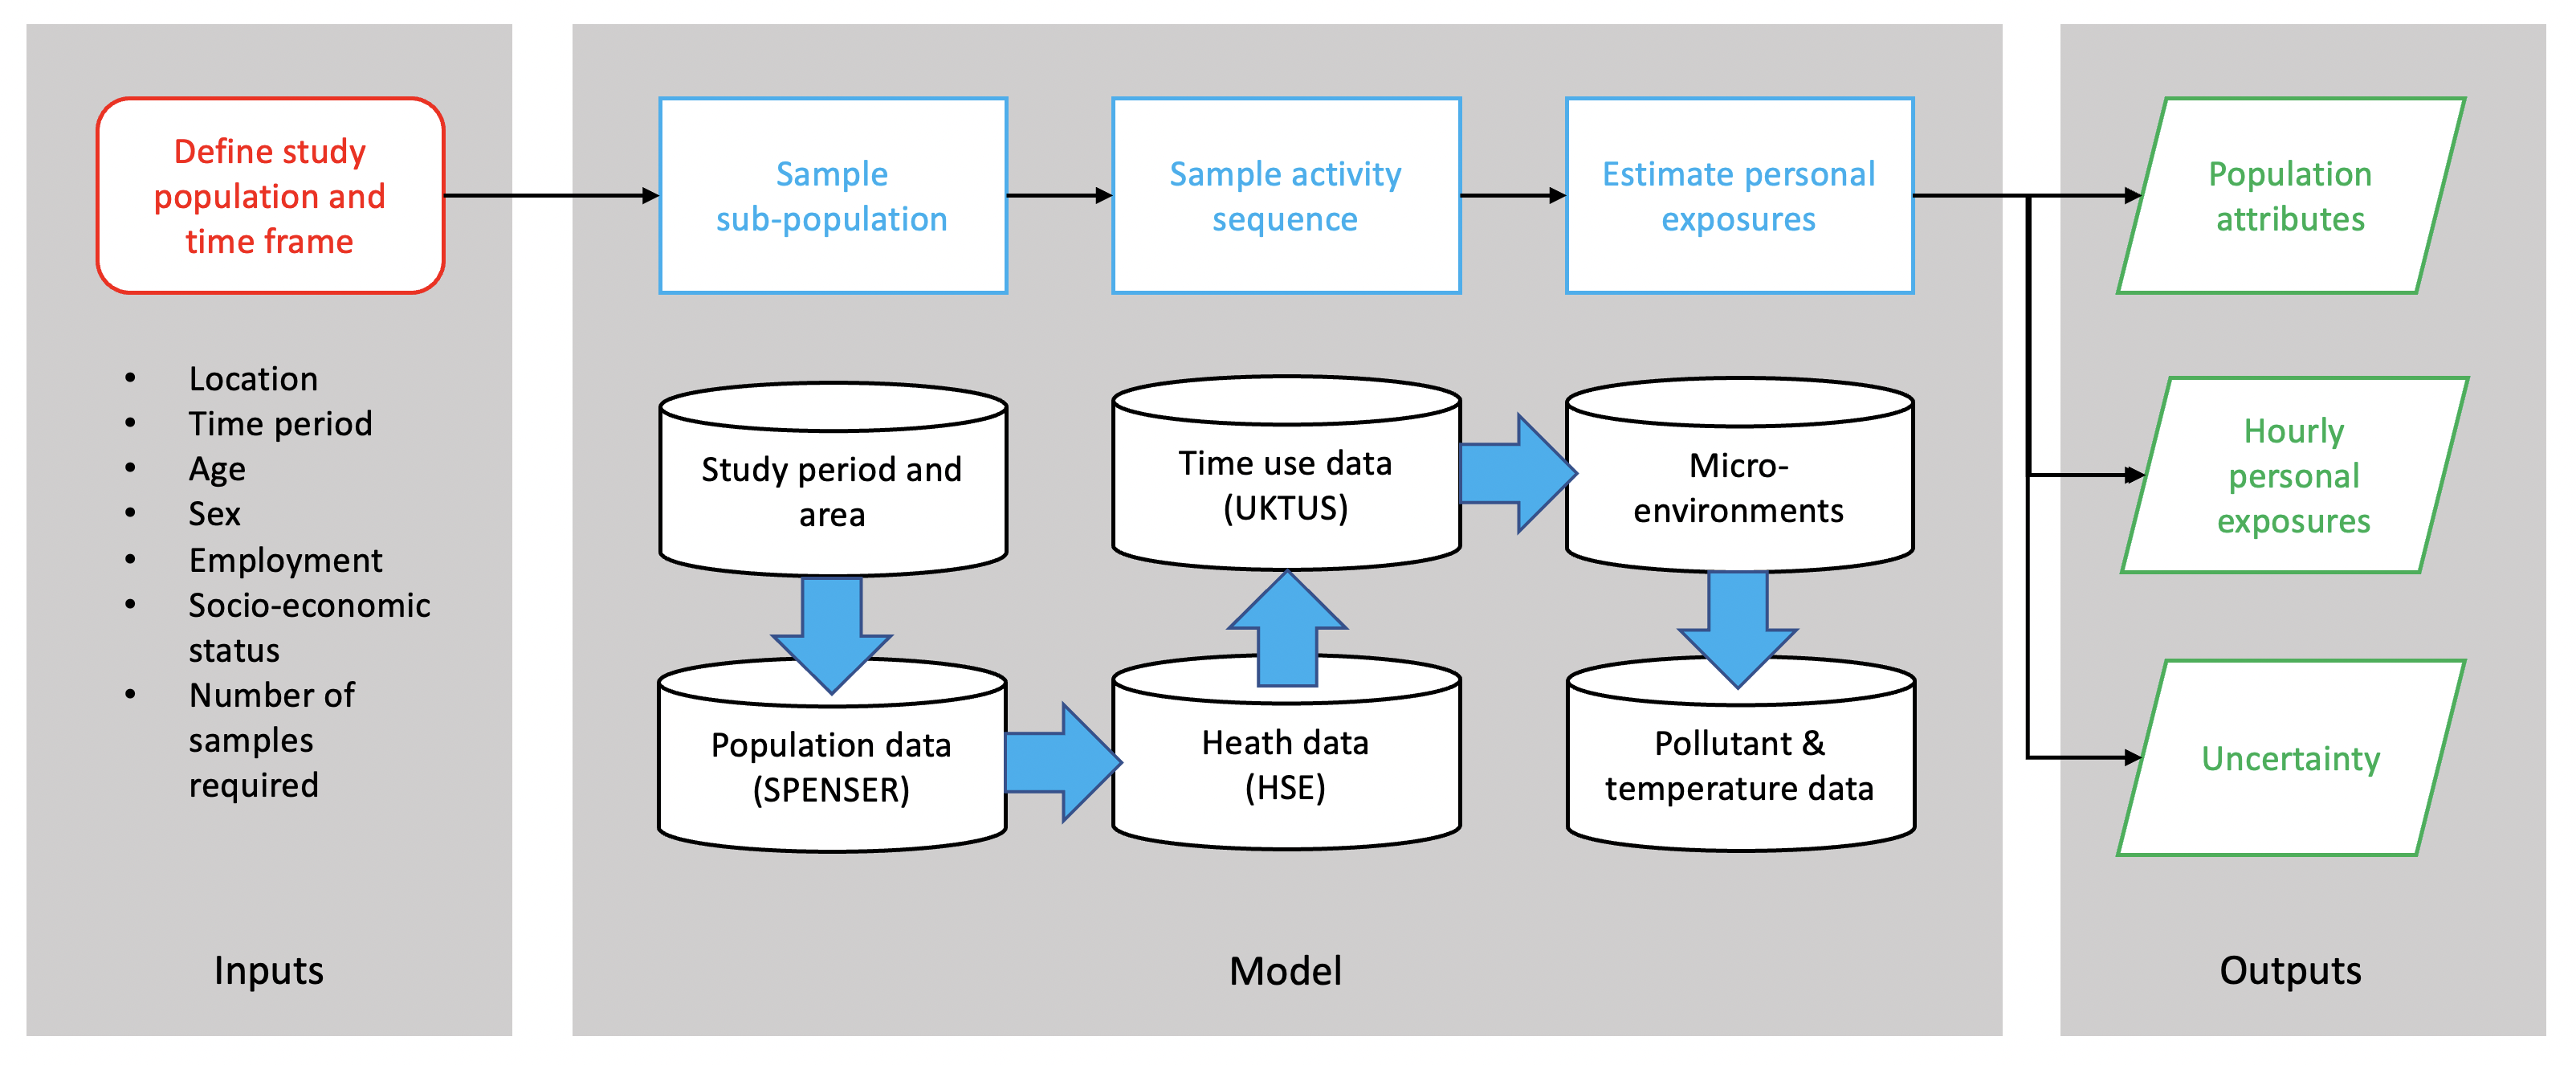
\includegraphics[width = 1.0\linewidth]{Figures/FlowChart3.png}
    \caption{Schematic of the Data Integration Model for EXposure process for simulating personal exposures for (sub-)populations.}
    \label{fig::schematic}
\end{figure}

A schematic of the process for simulating personal exposures for (sub-)populations can be seen in Figure \ref{fig::schematic}. It  comprises of five inter-linked processes:

\begin{enumerate}
    \item {\bf  Define study population and time frame} Definition of a specific (sub-)population and time interval of interest  The population of interest may be defined on multiple demographic variables such as sex, age group and employment status. 
    \item{\bf Sample sub-population} For the location and time period of interest,  individuals are extracted from the synthetic population database 
    \item {\bf Sample activity sequence}  Information on the individuals are extracted from a collection of databases and the data is processed and prepared for modelling. An activity sampler used to create a series of activity sequences for each individual.
    \item{\bf Estimate personal exposures}  The time each individual spends in a series of micro-environments generated from the activity sampler are matched with corresponding concentrations of air pollution  to obtain exposures.
    \item{\bf Outputs}  Samples of exposures for each individual are output and can be summarised at varying levels of aggregation over space and time. 
\end{enumerate}

%%%%%%%%%%%%%%%%%%%%%%%%%%%%%%%%%%%%%%%%%%%%%%%%%%%%%%%%%%%%%%%%%%
%%%%%%%%%%%%%%%%%%%%%%%%%%%%%%%%%%%%%%%%%%%%%%%%%%%%%%%%%%%%%%%%%%
\clearpage
\subsection{Synthetic Population}\label{sec::spenser}

%%%%%%%%%%%%%%%%%%%%%%%%%%%%%%%%%%%%%%%%%%%%%%%%%%%%%%%%%%%%%%%%%%
%%%%%%%%%%%%%%%%%%%%%%%%%%%%%%%%%%%%%%%%%%%%%%%%%%%%%%%%%%%%%%%%%%

Within DIMEX, individuals are sampled from an underlying {\em synthetic} population from the area of interest. The synthetic population is created using the baseline data generated by the SPENSER spatial microsimulation model (Lomax et al., 2017). SPENSER combines census data with small scale surveys and datasets to create a geo-referenced synthetic population forecast for England and Wales at a high resolution (individual and household level) \citep{lomax2017microsimulation, smith2018ukpopulation}. Such  spatial microsimulation techniques have previously been used widely in financial and economic policy analysis \citep{tanton2018spatial} and are  increasingly being used in the analysis of public health \citep{spooner2021dynamic, morrissey2015mental}.\\

\noindent DIMEX uses the outputs of the Synthetic Population Estimation and Scenario Projection Model (SPENSER) developed by the University of Leeds and The Alan Turing Institute \citep{ATI}.  SPENSER uses Iterative Proportional Fitting \citep{lovelace2015evaluating} to reweight microdata and area level counts from the 2011 Census of Population for England and Wales to create a micro-level synthetic dataset for the entire population and comprises of four steps; (i) estimate the synthetic individuals, (ii) estimate household population; (iii) forecast baseline population forward into 2020 and (iv) assign synthetic individuals to households. For further details, see \citep{lomax2017microsimulation, smith2018ukpopulation}.  The dataset created by SPENSER contains demographic (age and sex), socioeconomic (household reference person) and housing condition variables for individuals within their composite households. Each individual is assigned to a Middle Layer Super Output Area (MSOA). MSOA is a census geography in which each area represents a mean population in the order of 7,200 individuals, and LSOA is a finer geography in the order of 1,500 individuals.\\

\noindent Synthetic individuals are assigned to a census geography called Middle Layer Super Output Area (MSOA) in which each area represents a mean population in the order of 7,200 individuals. Individuals are also attributed demographic (age and sex), socioeconomic (based on the socioeconomic status of the household's reference person) and housing condition variables. In total, there are an estimated 56 million individuals for England in 2020 contained in SPENSER. These individuals were extracted and the estimated population counts in each MSOA can be seen in Figure \ref{fig::SPENSER}. \\

\begin{figure}[ht]
    \centering
    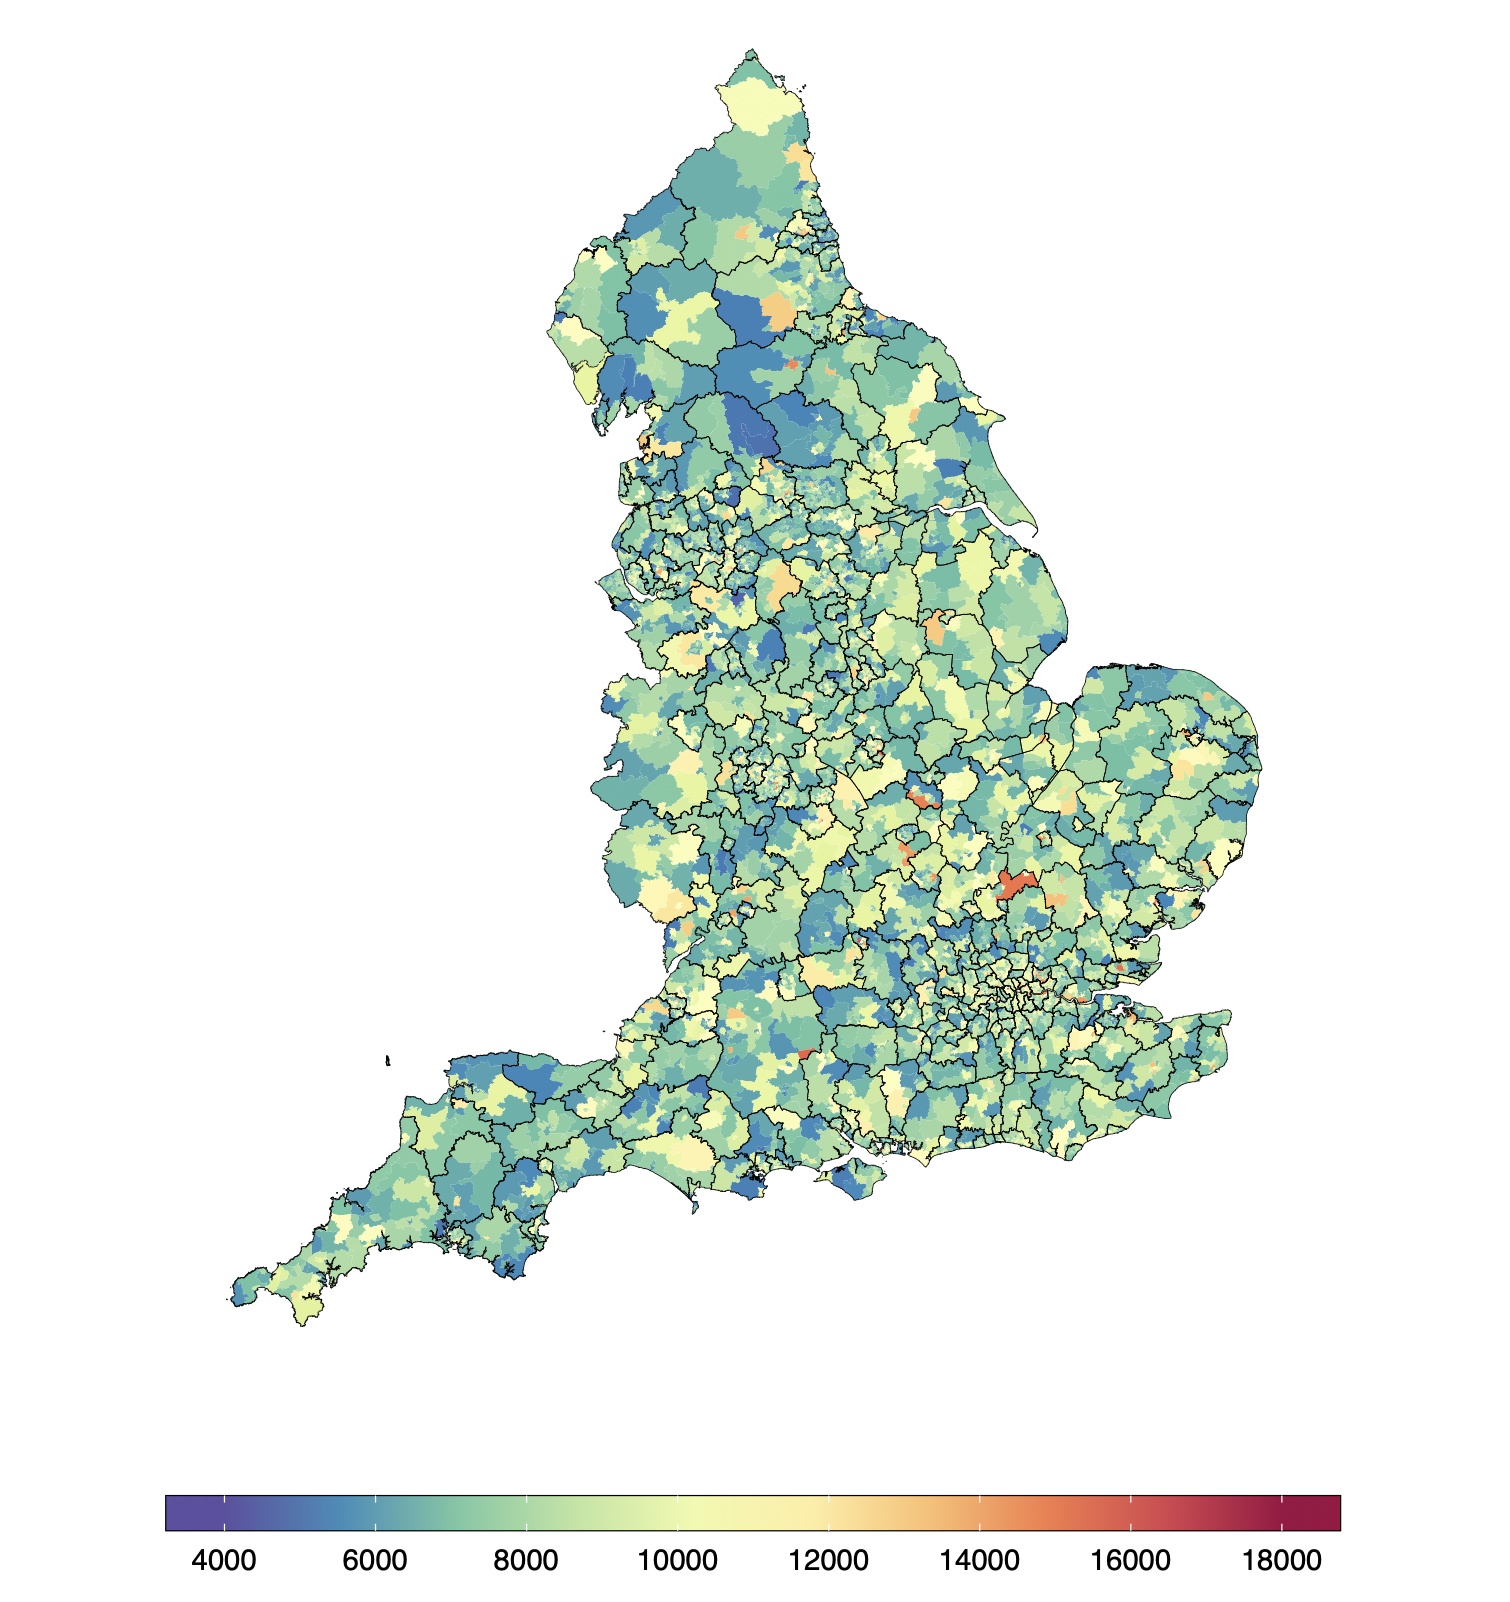
\includegraphics[width = 12cm]{Figures/SPENSER-England.png}
    \caption{Estimated 2020 population counts by Middle Layer Super Output Area (MSOA) in England from SPENSER. Colours represent the level of population. and the black lines represent the local authority boundaries in England. In total, there is an estimated 56 million synthetic individuals in England.} \label{fig::SPENSER}
\end{figure}

\noindent Based on the approach used in \citet{morrissey2015mental}, propensity score matching (PSM) using a kernel density algorithm was used to match each individual simulated by the SPENSER model to be matched to an individual in two external datasets based on the similarity of their demographic, socioeconomic and spatial characteristics. PSM was used to supplement the SPENSER dataset to include data from the United Kingdom Time Use Survey, 2014/2015 (UKTUS, \cite{uktus}) and the Health Survey of England, 2019 (HSE). \\

\noindent The UKTUS is a large-scale nationally-representative household survey and provides the richest source data on how people aged eight years and over in the UK spend their time, where they spend their time, and who they spend their time with. Surveyed individuals were asked to record information on their daily activities in diaries over the space of two weeks. Each diary consists of a sequence of starting times, durations and the location where the activities took place between 4am to 4am in 10-minute intervals. Furthermore, detailed employment information including information on employment status, industrial sector and occupation category (for those in employment) or previously in employment (i.e. they are now retired) were also recorded. The UKTUS also has detailed employment information as part of it's core set of questions including information on employment status, and industrial sector and occupation category for those in  employment or previously in employment (i.e. they are now retired). Including employment data and the occupation and industrial sector in which individuals are employed in, is important as it allows the identification of key workers in the dataset. \\

\begin{table}[ht]
 \caption{Attributes from the Synthetic Population Estimation and Scenario Projection Model (SPENSER) and variables from the United Kingdom Time Use Survey (UKTUS) and the Health Survey of England (HSE) added using propensity score matching}
  \centering
\begin{tabular}{|l|c|c|c|} 
 \hline
 
  \textbf{Variable} & \textbf{SPENSER} & \textbf{UKTUS} & \textbf{HSE} \\ 
\hline
\emph{ Individual}  &  &  & \\ \hline 
Sex & \checkmark & \checkmark & \checkmark \\ 
Age & \checkmark & \checkmark & \checkmark \\ 
Ethnicity & \checkmark &  & \checkmark \\ 
National Statistics Socio-economic Status   & \checkmark & \checkmark & \checkmark \\
(NS-SEC) of household reference person &  &  &  \\
Number in household & \checkmark &  &  \\
Time use data  &  & \checkmark &  \\
(proportion of time doing different activities) &  &  &  \\
Health data  &  &  & \checkmark \\
(CVD, high blood pressure, diabetes, &  &  &  \\
COPD, BMI$>$40) &  &  &  \\
In-work status  &  & \checkmark &  \\
Standard Industrial Classification of &  & \checkmark &  \\
economic activities (SIC) &  & \checkmark &  \\ \hline
\emph{ Household}  &  &  &\\ \hline
Type of dwelling inhabited  & \checkmark &  &  \\
(e.g. semi-detached house) & \checkmark &  &  \\
Tenure 	(e.g. rented, mortgaged) & \checkmark &  &  \\
Household Composition (e.g. cohabiting couple) & \checkmark &  &  \\
Number of occupants  & \checkmark &  &  \\
Number of rooms  & \checkmark &  &  \\
Presence of central heating & \checkmark &  &  \\
Type of dwelling & \checkmark &  &  \\
Number of cars in household  & \checkmark &  &  \\
 \hline
\end{tabular}
  \label{tab:spenserdata}
\end{table}

\noindent The HSE monitors trends in the nation’s health and care. It provides information about adults aged 16 and over, and children aged 0 to 15, living in private households in England. The survey is used to monitor the rate of obesity and to estimate the proportion of people in England who have certain health conditions and the prevalence of risk factors and health related behaviours, such as smoking and drinking alcohol. The additional variables matched to the outputs from SPENSER can be seen in Table \ref{tab:spenserdata}.\\

The following provides a summary of the validation of the matching process, further details can be found in the Supplementary Material of \cite{spooner2021dynamic}. Validation of the model outputs was performed via a series of balance tests \citep{Jesmin2012} where balance (in the context of PSM) is defined as the similarity between the multivariate empirical distributions of the covariates in the two datasets being matched (the synthetic population from SPENSER and the UKTUS / HSE) \citep{Rosenbaum1984}. Balance was assessed using pseudo R2, p-score and chi-squared test statistics.  ‘Good balancing’ indicates  no systematic difference in the distribution of covariates between the two groups. Performance in terms of these metrics  using a selection of  different approaches, a kernel, nearest neighbours and local linear regression algorithms, with the former slightly out-performed the second two approaches.  Based on this appraisal, the kernel-matching algorithm was chosen to perform the overall match. Every matched individual in SPENSER dataset had the same sex age-band, ethnicity and household reference NS-SEC as their matched counterpart in the UKTUS dataset. Once the SPENSER dataset has been augmented with the UKTUS data, the HSE data is then matched to the SPENSER model using age, sex and NS-SEC variables. \\


%%%%%%%%%%%%%%%%%%%%%%%%%%%%%%%%%%%%%%%%%%%%%%%%%%%%%%%%%%%%%%%%%%
%%%%%%%%%%%%%%%%%%%%%%%%%%%%%%%%%%%%%%%%%%%%%%%%%%%%%%%%%%%%%%%%%%
\clearpage
\subsection{Activity sampler}\label{sec::activity}

%%%%%%%%%%%%%%%%%%%%%%%%%%%%%%%%%%%%%%%%%%%%%%%%%%%%%%%%%%%%%%%%%%
%%%%%%%%%%%%%%%%%%%%%%%%%%%%%%%%%%%%%%%%%%%%%%%%%%%%%%%%%%%%%%%%%%

An activity sampler samples and assigns sequences of micro-environments, representing daily routines, to individuals from the population and study area of interest. Here, activity sequences contain 24 elements, one for each hour of the day, with individuals moving through these micro-environments as the day progresses. Individuals only visit one micro-environment each hour of the day, thus cannot change environments within the hour. It is also assumed that individuals and the micro-environments they visit are always at the same geographical location in which they reside (i.e. the MSOA).  \\

\noindent The activity sequence of an sampled individual can be used to generate a \emph{ local array} \citep{zidek2007framework} for the series of micro-environments that a sampled individual moves between when completing different activities. This information was obtained from the UKTUS for which variables including age, sex, employment status, National Statistics Socio-economic classification (NS-SEC5), primary activities undertaken (in 10 minute intervals), survey weights and the corresponding location of the activities were extracted. The UKTUS is a nationally representative survey of time-use for individuals across the UK. In total, 15,058 activity diaries relating to for 7,543 respondents were extracted from the UKTUS for use in this analysis. The locations of each activity from the activity diaries were categorised into four micro-environments considered in this analysis: (i) "Home", (ii) "Indoor-not-home", (iii) "Outdoor" and (iv) "Transport" as described in Table \ref{tab::groupings}. Figure \ref{fig::TimeUseExamples} shows eight examples of  activity sequences (or local arrays), highlighting the paths followed by surveyed individuals through time. \\

\noindent Activity diaries was summarised to estimate the proportion of the day spent at Home, Indoor-not-home, Outdoor and Transport with results stratified by age group (<18, 18-29, 30-44, 45-59, 60-74 and 75+), sex, NS-SEC5, day type (weekday/weekend), season (Autumn, Winter, Spring, Summer) which can be seen in Table \ref{tab::summarydailydiaries}. Overall, surveyed individuals typically spent ca. 80\% (IQR: 59.9\% to 91.7\%) of their day at home, however there was considerable variation across age groups; with individuals aged 18-29 spending 63.2\% (IQR: 48.6\% to 83.3\%) of their time at home and individuals aged 75+ spending 91.7\% (IQR: 82.6\% to 100\%) of their day at home, due to the amount spent at work and other indoor-not-home locations. Furthermore, surveyed females typically spent more of their day at home than males (77.1\% vs. 70.8\% respectively), surveyed individuals spent more time at home during the weekend than during the weekday (79.2\% vs. 67.4\% respectively) and surveyed individuals spent more time at home during Autumn/Winter than in Spring/Summer. The majority of surveyed individuals did not spend any of their time outdoors which is consistent across age groups, sex, socio-economic classification and season. The proportion of the day spent in transport ranged from 0.7\% to 4.9\% with a median value of 3.5\% across all surveyed individuals. \\

\noindent Activity diaries were also summarised to estimate the proportion of surveyed individuals in each of the four micro-environments in each of the 10-minute intervals by age group and day type  which can be seen in Figure \ref{fig::propageday}. Overall, daily habits are similar across all surveyed individuals. Over 90\% reside at home until around 6am, at which point individuals leaving for work and other activities (such as leisure, school etc.). The percentage of surveyed individuals outside of their home peaks between 10am and 4pm and steadily declines until 10pm when the vast majority of individuals are back inside their homes. Again, we see that the proportion of people leaving their homes during the day varies considerably by age group, with older people spending more time indoors. Furthermore, we also see that habits are different between weekdays and the weekend, where surveyed individuals stated they remained in their homes. \\

\begin{figure}[!htbp]
	\centering
	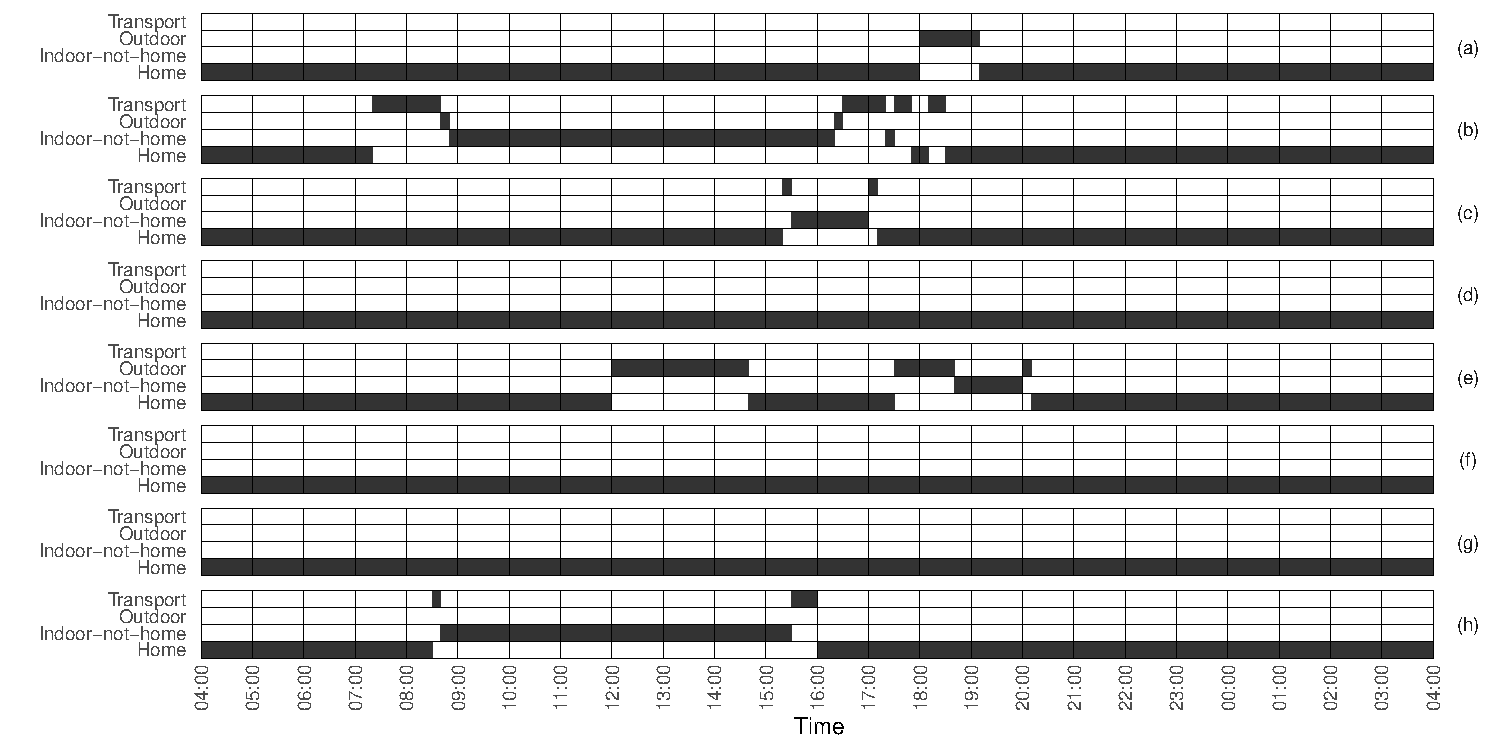
\includegraphics[width=\linewidth]{Figures/TimeUseExamples}	
	\caption{Example activity sequences in 10 minute intervals; (a) a full-time working female, during the weekend, (b) a full-time working female, during a weekday, (c) a retired male, during the weekend, (d) a retired male, during a weekday, (e) an unemployed male, during the weekend, (f) an unemployed male, during a weekday, (g) a school-child, during the weekend, (h) a school-child, during a weekday at term-time. Activities have been grouped by Home, Indoor-not-home, Transport and Outdoor.} \label{fig::TimeUseExamples}
\end{figure}

\begin{figure}[!htbp]
	\centering
	\includegraphics[width=0.95\linewidth]{Figures/TimeUse_AgeGr_DayType}	
	\caption{Proportion of surveyed individuals at Home, Indoor-not-home, Outdoor, Transport and Unknown locations by age group and day type from time activity diaries extracted from the UKTUS.}
	\label{fig::propageday}
\end{figure}


\begin{table}[ht]
\centering
\caption{Groupings of time activity locations into (a) Home, (b) Indoor-not-home, (c) Outdoor and (d) Transport.}\label{tab::groupings}
\begin{tabular}{ll}
  \hline
Group & Location \\ 
  \hline
Home & Home \\ 
   & Other peoples home \\ 
   & Second home or weekend house \\ 
  Indoor-not-home & Arts or cultural centre \\ 
   & Hotel guesthouse camping site \\ 
   & Other specified location (not travelling) \\ 
   & Restaurant cafe or pub \\ 
   & Shopping centres markets other shops \\ 
   & Sports facility \\ 
   & Working place or school \\ 
  Outdoor & Parks countryside seaside beach or coast \\ 
   & Travelling by bicycle \\ 
   & Travelling on foot \\ 
  Transport & Other specified private travelling mode \\ 
   & Other specified public transport mode \\ 
   & Travelling by aeroplane \\ 
   & Travelling by boat or ship \\ 
   & Travelling by bus \\ 
   & Travelling by coach \\ 
   & Travelling by lorry or tractor \\ 
   & Travelling by moped motorcycle or motorboat \\ 
   & Travelling by passenger car - driver status unspecified \\ 
   & Travelling by passenger car as a passenger \\ 
   & Travelling by passenger car as the driver \\ 
   & Travelling by taxi \\ 
   & Travelling by train \\ 
   & Travelling by tram or underground \\ 
   & Travelling by van \\ 
   & Unspecified private transport mode \\ 
   & Unspecified public transport mode \\ 
   & Unspecified transport mode \\ 
   & Waiting for public transport \\ 
  Unknown & Illegible location or transport mode \\ 
   & No answer/refused \\ 
   & Unspecified location \\ 
   & Unspecified location (not travelling) \\ 
   \hline
\end{tabular}
\end{table}

\begin{landscape}
\begin{table}[ht]
\centering
\caption{Summary of time spent at Home, Indoor-not-home, Outdoor and Transport from time activity diaries extracted from the UKTUS. Results are presented using medians and interquartile range (IQR), stratified by Age group, Sex, NS-SEC5, Day type and Season. Results are weighted by individual survey weights to ensure summaries are representative of the UK population.}\label{tab::summarydailydiaries}
\begin{tabular}{llccccccccc}
  \hline
  \hline\\[-8pt]
  % & & & \multicolumn{8}{c}{\textbf{Time spent in each environment (\%)}} \\
	 % \cmidrule(lr){4-11}
   & & & \multicolumn{2}{c}{\textbf{Home}}& \multicolumn{2}{c}{\textbf{Indoor-not-home}} & \multicolumn{2}{c}{\textbf{Outdoor}} & \multicolumn{2}{c}{\textbf{Transport}}\\
	 \cmidrule(lr){4-5}
	 \cmidrule(lr){6-7}
	 \cmidrule(lr){8-9}
	 \cmidrule(lr){10-11}
   & & n & Median & IQR & Median & IQR & Median & IQR & Median & IQR  \\ 
  \hline
 \multicolumn{2}{l}{\textbf{Total}} & 15058 & 79.2\% & (59.7\% - 91.7\%) & 9.0\% & (0.0\% - 28.5\%) & 0.0\% & (0.0\% - 3.5\%) & 3.5\% & (0.7\% - 6.9\%) \\[3pt] 
 \multicolumn{2}{l}{\textbf{Age}} \\
   & $<$18 & 1944 & 69.4\% & (59.0\% - 86.1\%) & 20.8\% & (4.9\% - 30.6\%) & 0.0\% & (0.0\% - 4.2\%) & 2.1\% & (0.0\% - 5.6\%) \\ 
   & 18-29 & 1979 & 63.2\% & (48.6\% - 83.3\%) & 25.0\% & (6.9\% - 40.3\%) & 0.0\% & (0.0\% - 3.5\%) & 4.2\% & (0.7\% - 7.6\%) \\ 
   & 30-44 & 3283 & 68.1\% & (54.2\% - 85.4\%) & 18.1\% & (5.6\% - 35.4\%) & 0.0\% & (0.0\% - 4.2\%) & 4.2\% & (1.4\% - 8.3\%) \\ 
   & 45-59 & 3697 & 70.8\% & (54.9\% - 86.8\%) & 16.0\% & (4.2\% - 34.0\%) & 0.0\% & (0.0\% - 3.5\%) & 4.2\% & (1.4\% - 8.3\%) \\ 
   & 60-74 & 2948 & 81.9\% & (66.7\% - 91.7\%) & 9.0\% & (0.7\% - 19.4\%) & 0.0\% & (0.0\% - 3.5\%) & 3.5\% & (0.0\% - 6.9\%) \\ 
   & 75+ & 1207 & 91.7\% & (82.6\% - 100.0\%) & 3.5\% & (0.0\% - 9.7\%) & 0.0\% & (0.0\% - 1.4\%) & 0.7\% & (0.0\% - 4.2\%) \\[3pt] 
 \multicolumn{2}{l}{\textbf{Sex}} \\
   & Female & 8075 & 77.1\% & (59.0\% - 90.3\%) & 12.5\% & (2.8\% - 29.2\%) & 0.0\% & (0.0\% - 3.5\%) & 3.5\% & (0.7\% - 6.9\%) \\ 
   & Male & 6983 & 70.8\% & (54.2\% - 87.5\%) & 16.0\% & (4.2\% - 34.7\%) & 0.0\% & (0.0\% - 3.5\%) & 3.5\% & (0.7\% - 7.6\%) \\[3pt] 
 \multicolumn{2}{l}{\textbf{NS-SEC5}$^\dagger$} \\
   & 0 & 3222 & 77.8\% & (63.2\% - 91.0\%) & 12.5\% & (0.7\% - 27.8\%) & 0.0\% & (0.0\% - 3.5\%) & 2.1\% & (0.0\% - 4.9\%) \\ 
   & 1 & 4429 & 70.1\% & (54.2\% - 86.8\%) & 16.7\% & (4.2\% - 35.4\%) & 0.0\% & (0.0\% - 3.5\%) & 4.2\% & (1.4\% - 8.3\%) \\ 
   & 2 & 2010 & 75.0\% & (56.2\% - 89.6\%) & 13.2\% & (4.2\% - 32.6\%) & 0.0\% & (0.0\% - 3.5\%) & 4.2\% & (1.4\% - 7.6\%) \\ 
   & 3 & 1161 & 74.3\% & (56.9\% - 88.2\%) & 12.5\% & (3.5\% - 31.9\%) & 0.0\% & (0.0\% - 3.5\%) & 4.2\% & (1.4\% - 8.3\%) \\ 
   & 4 & 572 & 63.9\% & (50.0\% - 86.9\%) & 21.5\% & (5.6\% - 38.9\%) & 0.0\% & (0.0\% - 2.1\%) & 4.9\% & (1.4\% - 7.8\%) \\ 
   & 5 & 3664 & 75.7\% & (57.6\% - 91.0\%) & 12.5\% & (2.1\% - 30.6\%) & 0.0\% & (0.0\% - 2.8\%) & 2.8\% & (0.0\% - 6.9\%) \\[3pt]
 \multicolumn{2}{l}{\textbf{Day type}} \\ 
   & Weekday & 7543 & 67.4\% & (54.2\% - 86.1\%) & 20.8\% & (4.9\% - 35.4\%) & 0.0\% & (0.0\% - 3.5\%) & 4.2\% & (0.7\% - 7.6\%) \\ 
   & Weekend & 7515 & 79.2\% & (61.8\% - 91.7\%) & 10.4\% & (1.4\% - 25.0\%) & 0.0\% & (0.0\% - 3.5\%) & 2.8\% & (0.0\% - 6.9\%) \\[3pt]
 \multicolumn{2}{l}{\textbf{Season}} \\
   & Autumn & 4466 & 74.3\% & (56.9\% - 89.6\%) & 14.6\% & (3.5\% - 33.3\%) & 0.0\% & (0.0\% - 3.5\%) & 3.5\% & (0.0\% - 6.9\%) \\ 
   & Spring & 3560 & 72.2\% & (54.9\% - 88.2\%) & 13.2\% & (2.8\% - 31.2\%) & 0.0\% & (0.0\% - 3.5\%) & 3.5\% & (0.7\% - 7.6\%) \\ 
   & Summer & 3620 & 72.9\% & (55.6\% - 88.9\%) & 13.9\% & (2.8\% - 31.9\%) & 0.0\% & (0.0\% - 4.2\%) & 3.5\% & (0.7\% - 6.9\%) \\ 
   & Winter & 3412 & 75.7\% & (59.0\% - 90.3\%) & 13.9\% & (3.5\% - 32.6\%) & 0.0\% & (0.0\% - 2.8\%) & 3.5\% & (0.7\% - 6.9\%) \\[3pt] 
   \hline
   \hline
   \multicolumn{11}{p{19cm}}{\textbf{$^\dagger$}\footnotesize 0 = Not applicable/Economically inactive, 1 = Higher managerial, administrative and professional occupations, 2 = Intermediate occupations, 3 = Small employers and own account workers, 4 = Lower supervisory and technical occupations, 5 = Semi-routine and routine occupations} \\
\end{tabular}
\end{table}
\end{landscape}

\noindent In the development of DIMEX, two different approaches to activity sampling were considered, with the difference being in the way that the sequences of activities, and the associated micro-environments (i.e. the local array) are constructed
\begin{itemize}
    \item[] \textbf{Method 1}: Following \citep{zidek2007framework}, activity sequences of an sampled individual from SPENSER are generated by concatenating randomly selected UKTUS diaries.
    \item[] \textbf{Method 2}: Extending the approach by \citep{zidek2007framework}, activity sequences are generated by recursively sampling micro-environments that an individual might make during the day at successive time points. Sampling was done by estimating (empirical) probabilities of transitioning between different micro-environments during the day, estimated by summarising the UKTUS diaries.
\end{itemize}
Both methods involve sampling different elements at successive time-points, creating a composite individual with more variable behavior than that of a single individual \citep{zidek2007framework}. Survey sample weights were utilised to ensure the randomly selected UKTUS diaries and the transition probabilities are representative of the UK general population. \\

\noindent Some UKTUS diaries contained missing locations, and to overcome this, three approaches were considered: (i) a complete case analysis where only complete UKTUS diaries were used, (ii) fill in missing locations using the most common location recorded when the same activity is recorded and (iii) similar to a multiple imputation, is to fill in missing locations by sampling from other locations where the same activity is recorded. \\

\noindent UKTUS diaries are recorded in 10-minute intervals and in order to create hourly sequence of micro-environments were implemented: (i) allocate the (hourly) micro-environment where the individual spent most of the hour and (ii) randomly select the (hourly) micro-environment proportional to the time spent in each micro-environment, the latter being the default methods used within DIMEX.

%%%%%%%%%%%%%%%%%%%%%%%%%%%%%%%%%%%%%%%%%%%%%%%%%%%%%%%%%%%%%%%%%%
%%%%%%%%%%%%%%%%%%%%%%%%%%%%%%%%%%%%%%%%%%%%%%%%%%%%%%%%%%%%%%%%%%
\clearpage
\subsection{Exposure estimation}

%%%%%%%%%%%%%%%%%%%%%%%%%%%%%%%%%%%%%%%%%%%%%%%%%%%%%%%%%%%%%%%%%%
%%%%%%%%%%%%%%%%%%%%%%%%%%%%%%%%%%%%%%%%%%%%%%%%%%%%%%%%%%%%%%%%%%

Each of the individuals activity sequence needs to be matched to the corresponding concentrations of air pollutions they are exposed to in each micro-environment. Following \citet{zidek2007framework}, local concentrations of air pollutants in each micro-environment are modelled as a function of the the ambient outdoor concentrations air pollution and non-ambient sources of air pollution
\begin{equation*}
	local = \Phi(ambient, source). 
\end{equation*}
Micro-environments belong to one of two categories: closed micro-environments and open micro-environments. Concentrations of PM$_{2.5}$ in closed micro-environments are assumed to come from both ambient and non-ambient sources, whereas concentrations of PM$_{2.5}$ in open micro-environments are assumed to only come from ambient sources of air pollution. Here, `home' is considered a closed micro-environment with `indoor not home', `transport', and `outdoor' considered as open micro-environments.  

%%%%%%%%%%%%%%%%%%%%%%%%%%%%%%%%%%%%%%%%%%%%%%%%%%%%%%%%%%%%%%%%%%
\clearpage
\subsubsection{Open micro-environments}

%%%%%%%%%%%%%%%%%%%%%%%%%%%%%%%%%%%%%%%%%%%%%%%%%%%%%%%%%%%%%%%%%%

The estimated concentration of PM$_{2.5}$, $Y_{mst}$, in open micro-environment $m \in \{1, \ldots, N_M\}$, location $s\in \{1, \ldots, N_S\}$ and time $t\in \{1, \ldots, N_T\}$ is modelled using as a linear transformation of the ambient concentration of PM$_{2.5}$, $X_{st}$, 
\begin{equation*}
	Y_{mst} = a_m + b_m\cdot X_{st}
\end{equation*}
Prior distributions for the parameters $a_m$ and $b_m$ in each of the open micro-environments are taken from scientific literature. Information for the `indoor not home' prior distributions combine estimates for work, school, and shopping from \citet{burke2001population}. Information for the `transport' prior distributions are also obtained from \citet{burke2001population}. It is assumed that the concentrations of PM$_{2.5}$ for `outdoor' micro-environments and the ambient concentrations are equal. Gaussian distributions are truncated at zero so that sampled values below zero are not simulated. The distributions used for $a_m$ and $b_m$ in each micro-environment $m$ can be seen in Table \ref{tab::openmicro}.

%%%%%%%%%%%%%%%%%%%%%%%%%%%%%%%%%%%%%%%%%%%%%%%%%%%%%%%%%%%%%%%%%%
\clearpage
\subsubsection{Closed micro-environments}\label{sec::micro}

%%%%%%%%%%%%%%%%%%%%%%%%%%%%%%%%%%%%%%%%%%%%%%%%%%%%%%%%%%%%%%%%%%

The estimated concentration of PM$_{2.5}$, $Y_{mst}$, in a closed micro-environment $m$ at time $t$, $C_m(t)$, is modelled using the mass balance equations. The mass balance equations links non-ambient sources of air pollution with the ambient outdoor air pollution and factors in characteristics of the environment such as the size and the amount of ventilation to estimate concentrations within the closed-micro-environment. They are as follows, 
\begin{equation*}
	\frac{d}{dt}Y_{mst} = \frac{S_{mt}}{V_m} + v_m\cdot F^p_m \cdot X_{st} - (v_m + F^d_m)\cdot Y_{mst}. 
\end{equation*}
Here, $X_{st}$ is the ambient outdoor concentration of PM$_{2.5}$, $S_t$ is the PM$_{2.5}$ emitted from non-ambient sources, $V_m$ is the volume of the micro-environment, $v_m$ is the air exchange rate between the closed micro-environment and ambient outdoor concentrations of PM$_{2.5}$, $F^p_m$ is the penetration factor, and $F^d_m$ is the deposition rate. The penetration factor and deposition rate define where the equilibrium of the mass balance equation lies while the air exchange rate defines how quickly this equilibrium is reached. \citet{zidek2007framework} found the following solution the mass balance equation, 
\begin{equation*}
	\begin{split}
		Y_{ms(t+u)} &= \frac{C}{v_m + F^d_m} + \left(Y_{mst} - \frac{C}{v_m + F^d_m}\right)\exp\left(-(v_m + F^d_m)u\right) \;\;\; u \in (0,1)\\
		C &\equiv \frac{S_{mt}}{V_m + F^d_m} + v_m\cdot F^p_m X_{st} 
	\end{split}
\end{equation*}
For further details on the mass balance equations, see \citet{zidek2003computational, zidek2007framework}. The mass balance equation is used here to produce hourly estimates of the concentrations of PM$_{2.5}$ in a `home' micro-environment and computation is started three days before the specified time frame for the equations to achieve equilibrium, with the a prior distribution of the concentration starting point taken from  \citet{wallace1993indoor}. \\

\noindent Information on housing volume, $V$, is taken from the property website Zoopla. A sample of 80 houses are taken from Zoopla and converted into a triangular distribution for the simulating the square footage and uniform distribution used for the ceiling height required to estimates the volume of the house. For the penetration factor, $F^p$, and the deposition rate, $F^d$ prior distributions are taken from \citet{burke2001population}. \\

\noindent Prior distributions for the air exchange rate, $v$, are taken from \citet{murray1995residential}. The air exchange rate is estimated for four different regions which are defined by the annual heating degree days, which are calculated by calculating the difference between the daily temperature and 18.3$^{o}$C and summed over an entire year. Temperature data for England in 2018 was obtained from the UK Automatic Urban and Rural Network (AURN) \citep{AURN} and it was found that England lies in region 3 and the corresponding priors were obtained. \\

\noindent The non-ambient sources of PM$_{2.5}$ used in the mass balance equations are restricted to smoking, cooking, and other sources that cannot directly be linked to a specific source (often called the personal cloud). For any given hour, the probability of a person cooking is arbitrarily chosen to be 0.1. If an individual cooks within the hour, then the PM$_{2.5}$ emitted is sampled from a prior distribution taken from \citet{ozkaynak1996personal}. If the individual is a smoker, then it is assumed that they smoke in 15 hours of the day. An hourly cigarette consumption is sampled from a prior distribution taken from the \citet{ONS2020}. The PM$_{2.5}$ emitted from smoking one cigarette is sampled from a prior distribution taken from \citet{ozkaynak1996personal} and multiplied to the hourly cigarette consumption to get a total PM$_{2.5}$ emitted from smoking. If an individual is a non-smoker it is assumed that there is not contact with PM$_{2.5}$ emitted by another individual smoking (i.e. there is no second-hand smoke). This is based on the data about smoking behaviour in the UK published by the Office for National Statistics showing an overall declining trend in smoking prevalence in addition to restrictions of smoking in public areas restrictions on smoking in public areas make exposure to PM$_{2.5}$ through second-hand smoke less likely. PM$_{2.5}$ emitted from other non-ambient sources is also sampled a from a prior distribution taken from the \citet{ONS2020}. The total non-ambient concentrations of PM$_{2.5}$ then consists of the sum of PM$_{2.5}$ emitted from these three sources. \\

\noindent The full list of prior distributions for the parameters used in the mass balance equations can be seen in Table \ref{tab::closedmicro}.

%%%%%%%%%%%%%%%%%%%%%%%%%%%%%%%%%%%%%%%%%%%%%%%%%%%%%%%%%%%%%%%%%%
%%%%%%%%%%%%%%%%%%%%%%%%%%%%%%%%%%%%%%%%%%%%%%%%%%%%%%%%%%%%%%%%%%
\clearpage
\subsection{Exposure simulator}

%%%%%%%%%%%%%%%%%%%%%%%%%%%%%%%%%%%%%%%%%%%%%%%%%%%%%%%%%%%%%%%%%%
%%%%%%%%%%%%%%%%%%%%%%%%%%%%%%%%%%%%%%%%%%%%%%%%%%%%%%%%%%%%%%%%%%

Individuals are sampled from the SPENSER population and using the methodologies described in Sections \ref{sec::activity} and \ref{sec::micro}, an exposure simulator is used to generate hourly activity sequences as well as the corresponding concentrations of PM$_{2.5}$ in each of the micro-environments. The simulator then matches the sequence of different micro-environments visited with the corresponding estimates of PM$_{2.5}$ which can then be used to summarise an the sampled population (or sub-populations) exposure to PM$_{2.5}$. 

%%%%%%%%%%%%%%%%%%%%%%%%%%%%%%%%%%%%%%%%%%%%%%%%%%%%%%%%%%%%%%%%%%
%%%%%%%%%%%%%%%%%%%%%%%%%%%%%%%%%%%%%%%%%%%%%%%%%%%%%%%%%%%%%%%%%%
%%%%%%%%%%%%%%%%%%%%%%%%%%%%%%%%%%%%%%%%%%%%%%%%%%%%%%%%%%%%%%%%%%
\clearpage
\section{Air pollution measurement, modelling and monitoring mobility}\label{sec::apmandm}

%%%%%%%%%%%%%%%%%%%%%%%%%%%%%%%%%%%%%%%%%%%%%%%%%%%%%%%%%%%%%%%%%%
%%%%%%%%%%%%%%%%%%%%%%%%%%%%%%%%%%%%%%%%%%%%%%%%%%%%%%%%%%%%%%%%%%
%%%%%%%%%%%%%%%%%%%%%%%%%%%%%%%%%%%%%%%%%%%%%%%%%%%%%%%%%%%%%%%%%%
\clearpage
\subsection{Network of sensor deployment}

%%%%%%%%%%%%%%%%%%%%%%%%%%%%%%%%%%%%%%%%%%%%%%%%%%%%%%%%%%%%%%%%%%
%%%%%%%%%%%%%%%%%%%%%%%%%%%%%%%%%%%%%%%%%%%%%%%%%%%%%%%%%%%%%%%%%%

Air quality in a specific location is a very complex result of local and regional emissions, atmospheric process that chemically and physically transform the primary pollutants and meteorology and accurate in-situ measurements are essential to monitor change. Low-cost air pollution sensors offer significant potential to improve both our understanding of, and ability to improve, urban air quality. These sensors therefore have the potential to provide the granularity of data to understand the effect of local interventions across the cities that are being led by regional authorities at scale, which are often implemented with an aim of improving air quality. With this in mind it is critical to monitor areas of Greater Manchester as interventions such as the Clean Air Zone are rolled out.  \\

\noindent As part of the project, and through leveraged funding from aligned projects, we have taken delivery of 10 Moduliar Gasses and PM. These units measure air quality including ozone (O$_3$), nitrogen monoxide (NO), nitrogen dioxide (NO$_{2}$), particulate matter of varying sizes (PM$_{1}$, PM$_{2.5}$, PM$_{10}$), wind speed/direction and noise. We have also taken delivery of 30 Modulair PM units. These units only measure PM$_{1}$, PM$_{2.5}$ and PM$_{10}$. \\

\noindent There are now a huge number of low-cost air quality monitoring approaches that, in the last 5 years seen a massive upsurge in use given their cost and very little requirement for prerequisite knowledge. Low-cost air pollution sensors offer significant potential to improve both our understanding of, and ability to improve, urban air quality. In contrast to traditional specialist sites and monitoring networks, where measurements are made using reference-grade equipment at a small number of locations, low-cost sensors offer the possibility of spatially dense observations that capture the spatial heterogeneity of air pollution. These sensors therefore have the potential to provide the granularity of data to understand the effect of local interventions that are being led by regional authorities and developers at scale, which are often implemented with an aim of improving air quality. The use of these devices is, however, being limited by questions over the data they provide and a lack of proven methodologies. \\

\noindent Academic scrutiny is unfortunately yet to provide a clear solution to the use of low-cost air pollution sensors, with a large degree of performance variability reported, even for identical devices. The reasons for these discrepancies are complex and wide-ranging, but have in a large part been attributed to interference from temperature and humidity or other gases, meaning performance often depends on local environmental conditions. For this reason, a long- term assessment of commercial low-cost air pollution sensor technologies has been underway across several UK cities since 2019, as part of the QUANT research programme. This study has deployed multiple commercial sensor devices, alongside reference-grade instruments, at the London and Manchester NERC supersites and a roadside monitoring site in York. This has enabled the assessment of the general performance of low- cost sensor devices in different UK urban environments and across a range of seasons and environmental conditions. \\

\noindent Figure \ref{fig::QUANT} shows \~1 month of PM$_{2.5}$ data from a reference equivalent FIDAS instrument and two low-cost sensor devices running at the Manchester NERC supersite. Although it is clear that the agreement between the low-cost devices and the FIDAS is not perfect, it is also obvious that the sensor signals do contain highly valuable information on local PM$_{2.5}$ levels and thus is a potentially valuable method of understanding air quality on a local scale. Through the quantification of these real-world low- cost sensor device uncertainties, the QUANT project allowed us to select and calibrate appropriate lower cost PM$_{2.5}$ measurement units to deploy across this project.\\

\begin{figure}
	\centering
	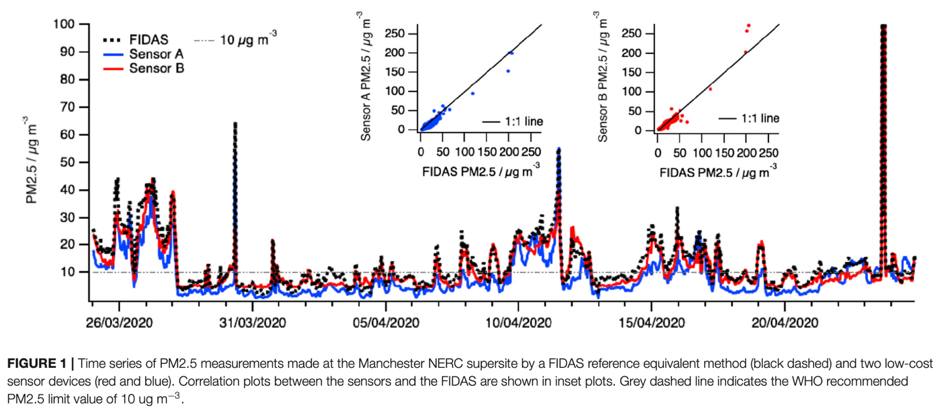
\includegraphics[width=0.95\linewidth]{Figures/QUANT_DIMEX.png}		
	\caption{Comparison between a reference grade instrument and low cost alternatives, informing selection and calibration units used across this project to fit DIMEX} \label{fig::QUANT}
\end{figure}

\noindent We also aligned with the collaborative deployment of mobility monitoring with Transport for Greater Manchester, to try and understand any regional-local patterns in varying modes of transport. For the focused LTn scheme we had acccess to 7 Vivacity cameras. These cameras measure movement around cities using object detection and compute vision technologies, giving measurements of vehicle, bike and pedestrian counts and exact path taken.
We also had access to 4 Black Cat Traffic Radars. This is a simpler traffic sensor based on radar technology, measuring traffic counts,
vehicle size. Predominantly useful for measuring speed of vehicles and not relevant for this study.

\noindent To integrate these units across the local urban estate, we have sourced power solution for lampposts and traffic light signals identified and purchases made. At the time of writing we have identified 20 sites for installations with TfGM and a further 10 sites with Manchester City council that are of interest scientifically. Our trial installations were completed with TfGM in the first week of February 22. This went well and has identified the method to internally wire up the sensors to traffic light signals at scale. Example data and the sensor set up is shown below. 

%%%%%%%%%%%%%%%%%%%%%%%%%%%%%%%%%%%%%%%%%%%%%%%%%%%%%%%%%%%%%%%%%%
%%%%%%%%%%%%%%%%%%%%%%%%%%%%%%%%%%%%%%%%%%%%%%%%%%%%%%%%%%%%%%%%%%
\clearpage
\subsection{AURN and new network of air quality sensor deployment}

%%%%%%%%%%%%%%%%%%%%%%%%%%%%%%%%%%%%%%%%%%%%%%%%%%%%%%%%%%%%%%%%%%
%%%%%%%%%%%%%%%%%%%%%%%%%%%%%%%%%%%%%%%%%%%%%%%%%%%%%%%%%%%%%%%%%%

Data from 3 AURN sites within the Greater Manchester region was used to profile seasonal profiles of PM$_{2.5}$ concentrations. An example of this is shown in figure \ref{fig::AURNexample}.\\

\begin{figure}
	\centering
	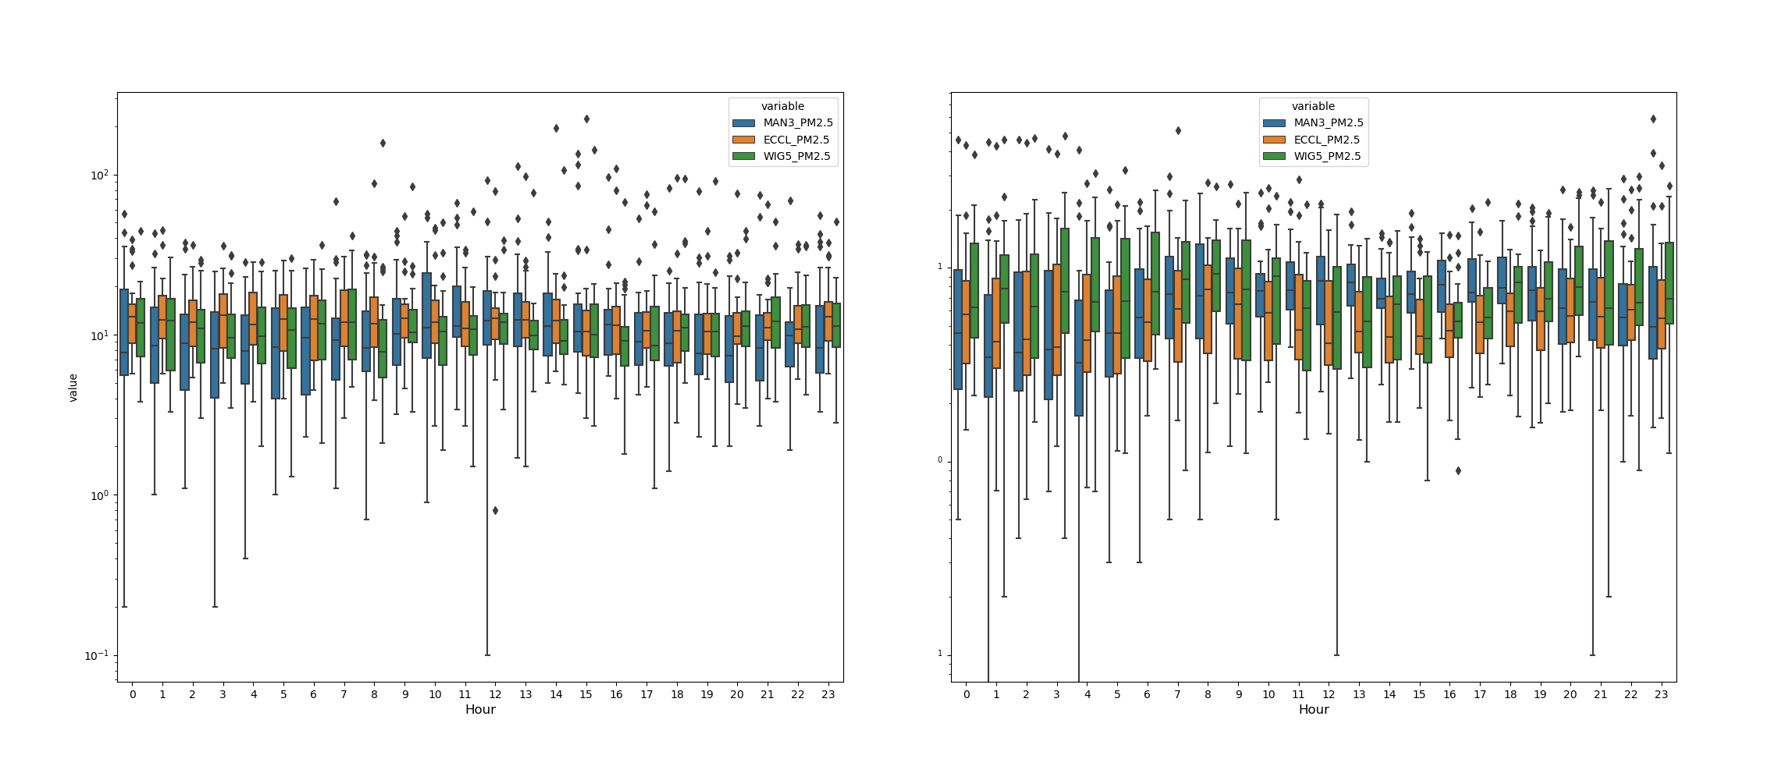
\includegraphics[width=0.95\linewidth]{Figures/profilespm25.png}		
	\caption{Example dirunal signature of PM$_{2.5}$ at the 3 Greater Manchester AURN sites for spring (left) and winter periods (right)} \label{fig::AURNexample}
\end{figure}

\noindent In addition, we have deployed, and continue to deploy, additional units across Manchester with and for our partners in Transport for Greater Manchester and Manchester City Council. Specifically we focused on a new Low Traffic Neighborhood scheme (LTN) in the Levenshulme area of South Manchester. The mean concentrations of NO, NO$_{2}$, O, PM$_{2.5}$ and PM$_{10}$ were measured across 5 sites of key concern in Levenshulme (Delamere Road, Grangethorpe Road, Manor Road, Slade Lane and Cromwell Grove) between April 2021 and October 2021. Levels for key pollutants NO$_{2}$  and PM$_{2.5}$ were compared to the mean air quality in Manchester and other comparable urban sites across the UK. This data was used to evaluate the geospatial discrepancies they may exist to inform personal exposure estimates. This is particularly important when integrating data from sparse networks of sensors. This also allows us to evaluate the change in time spent in different environments given an LTN may create a shift in mobility. In response, to supplement the air quality measurements, we were able to co-locate Vivacity cameras  that capture traffic volume and type. Analysis of five sites (Errwood Road, Crossley Road, Chapel Street, Rostron Road and Chapel Street Primary) with baseline data suggest that there have been marginal increases in car traffic of 3\%, strong increases in walking of 31\%, and a 108\% increase in cycling. The share of active transport, i.e. walking and cycling, increases from 22\% to 28\%, while the share of journeys taken by car decreases from 78\% to 72\%. Increases in walking and cycling at these sites suggests that the scheme has increased active transport across the area as a whole, as these comparison sites sit outside of the areas that would be expected to benefit from reduced traffic.  \\

\noindent Analysis showed that air quality in Levenshulme is broadly in line with levels across Manchester, though lower on average (figure \ref{fig::AURN}). In this figure, our measurement sites are shown in red, compared to the mean air quality in Manchester (green) and other comparable urban sites across the UK (grey) over 7 months of measurements. The red dots show the previous 5-year average level at each site, with most UK sites showing reductions due to Covid-19 restrictions. Please note red dots are only available for the AURN sites as they have been monitored as part of a long term national programme. The World Health Organisation global air quality thresholds released in 2021 are shown by the red horizontal line.  This does highlight the importance of investigating regional variation, as we discuss in the following section when using the EMEP model to provide those estimates at 1km resolution. \\

\noindent This suggests that the Levenshulme scheme has not had significant impacts.  NO$_{2}$ is more concerning than PM in terms of exceeding new WHO recommended levels. Traffic levels before and after the implementation of the phase 1 scheme suggest major increases in walking and cycling on roads that have been filtered as well as roads that are inside the general filtered area. There is evidence that the modal share on treated roads is approaching the 2040 TfGM target for <50\% of journeys to be by car. Traffic increases on boundary roads are modest and in line with broader regional trends in traffic levels between 2020 and 2021, suggesting that the scheme has not displaced large amounts of traffic onto these roads.

\begin{figure}
	\centering
	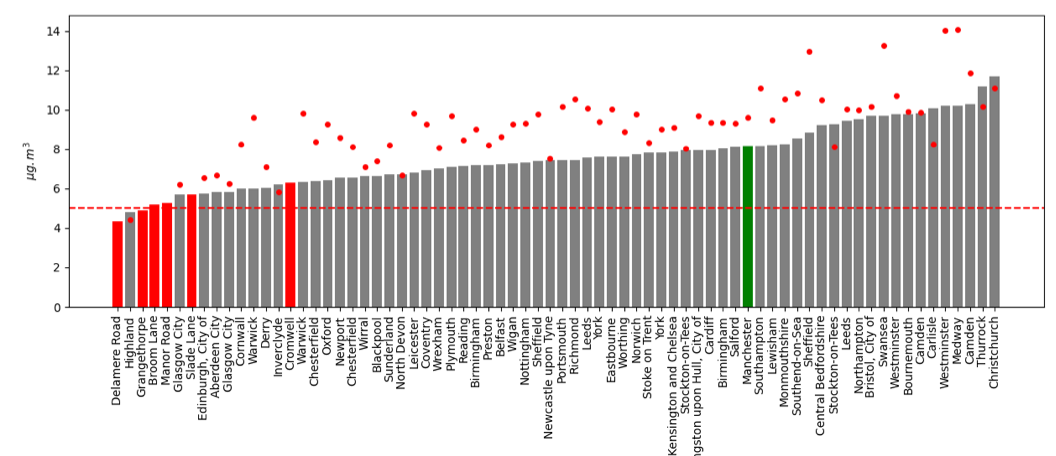
\includegraphics[width=0.95\linewidth]{Figures/levvy_aurn.png}		
	\caption{Mean PM$_{2.5}$ concentration at the measurement sites in Levenshulme between April 2021 and October 2021, shown in red. Mean concentration measured across Manchester is shown in green and other comparable sites in the UK as measured by the AURN sites are in grey.} \label{fig::AURN}
\end{figure}

%%%%%%%%%%%%%%%%%%%%%%%%%%%%%%%%%%%%%%%%%%%%%%%%%%%%%%%%%%%%%%%%%%
%%%%%%%%%%%%%%%%%%%%%%%%%%%%%%%%%%%%%%%%%%%%%%%%%%%%%%%%%%%%%%%%%%
\clearpage
\subsection{Mobility monitoring}

%%%%%%%%%%%%%%%%%%%%%%%%%%%%%%%%%%%%%%%%%%%%%%%%%%%%%%%%%%%%%%%%%%
%%%%%%%%%%%%%%%%%%%%%%%%%%%%%%%%%%%%%%%%%%%%%%%%%%%%%%%%%%%%%%%%%%

Data for the overall increase in traffic across Manchester between 2020 and 2021 is not available. DfT and gov.uk records run up to 2020 currently. Provisional road traffic estimates for Great Britain from October 2020 to
September 2021 suggest traffic on minor roads increased by 1.1\%. Figure xx compares the trend in traffic on our study sites with broader trends in traffic across Manchester and with a comparable site at Chester Road, Manchester. This graph was created as follows. Data from Apple routing requests has been made available to support Covid-19 studies across the UK. This data provides regional insight into changes in mobility through patterns in Apple routing requests in private vehicles and by cyclists. Traffic volume data from Chester Road is available from the same period from TfGM Drakewell database; a major route in and out of Manchester City centre. The data shown in Figure \ref{fig::travel1} represents changes in routing requests and volume respectively from both sources; a value of 100 represents the daily value on 1/12/20. To include data from Levenshulme we took the following approach. Traffic data from Grangethorpe was available from the same start date, shown on the plot as the solid purple line. All other roads are captured by the same methodology, referencing the daily sum on Grangethorpe on 1st Dec 2020. The data from the Levenshulme sites thus represent percentage change relative to Grangethorpe. The pattern of traffic on Grangethorpe seems to track broader levels across Manchester, and are very similar to those seen on the Chester Road. Many of the roads seem to show slight relative decreases against a background increase in Manchester. There is no evidence from these comparisons that the Levenshulme Active Neighbourhood scheme negatively impacted traffic levels on boundary and through roads in the area. \\

\begin{figure}
	\centering
	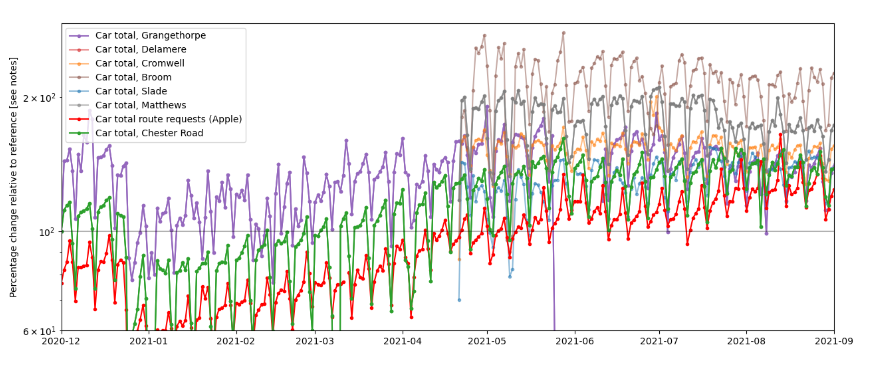
\includegraphics[width=0.95\linewidth]{Figures/routing_requests.png}		
	\caption{Comparing percentage change in car traffic relative to reference point for key study sites against route requests across Manchester
and a comparable site at Chester Road, December 2020 – October 2021} \label{fig::travel1}
\end{figure}

\noindent Figure \ref{fig::travel2} compares traffic levels across other comparable cities, including Sheffield, Newcastle and Hull, between February 2020 and February 2022. The section of the graph from December 2020 to September 2021 represents the time period included in Figure \ref{fig::travel1} above. Similar patterns can be observed across these other cities to those shown by the Apple routing data for Manchester and the Chester Road levels.\\

\begin{figure}
	\centering
	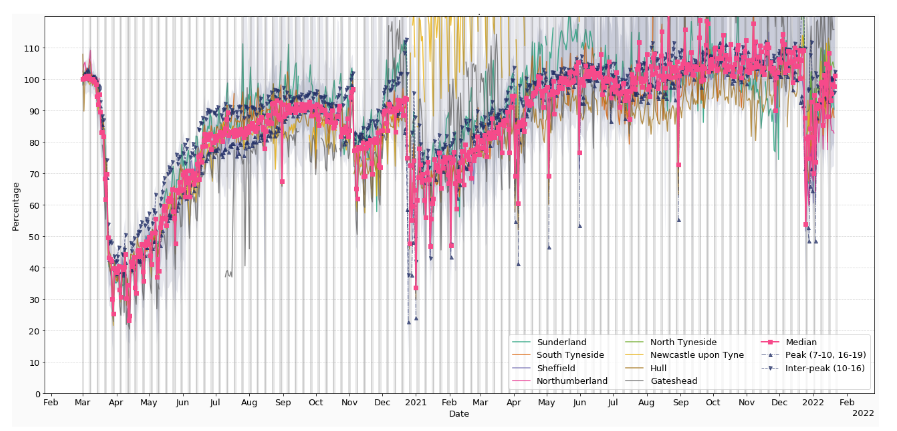
\includegraphics[width=0.95\linewidth]{Figures/routing_newcastle.png}
	\caption{Traffic volumes from 694 monitoring sites across Tyne and Wear, Hull and Sheffield, relative to a pre-lockdown baseline of 100.
Bank holidays and weekends are shaded (https://covid.view.urbanobservatory.ac.uk/output/plot-summary-of-traffic-volumes-no10.html)} \label{fig::travel2}
\end{figure}

\noindent The data indicates that traffic levels are remarkably consistent at a number of study sites throughout the day. In addition, two of the study sites are adjacent to primary schools. The data reveals heavy usage of these streets by pedestrians at school drop off and pick up times. Figure \ref{fig::school1} and Figure \ref{fig::school2} below show different classes of street user in 15 minute totals across a typical day on the 30th of April 2021.\\

\begin{figure}
	\centering
	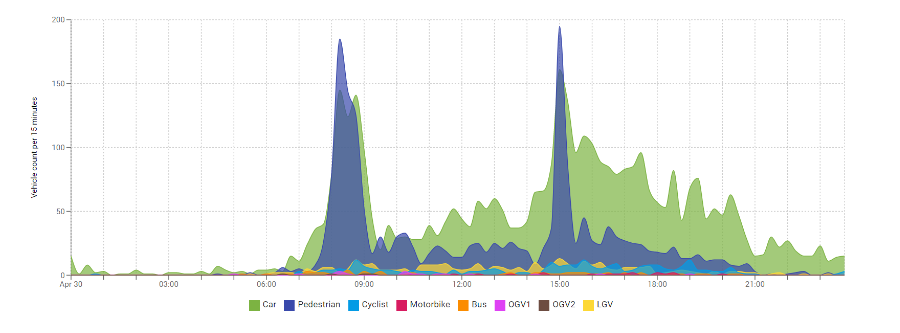
\includegraphics[width=0.95\linewidth]{Figures/mobility_school.png}
	\caption{User classes per 15 minutes for Errwood Road, 30/04/2021} \label{fig::school1}
\end{figure}

\begin{figure}
	\centering
	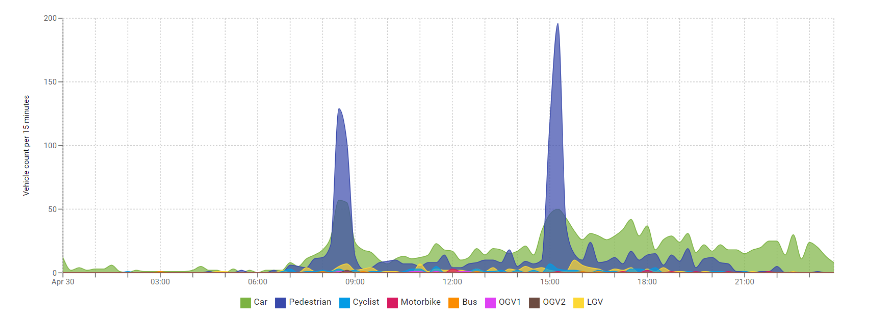
\includegraphics[width=0.95\linewidth]{Figures/mobility_school2.png}
	\caption{User classes per 15 minutes for Chapel Street, 30/04/2021} \label{fig::school2}
\end{figure}

\noindent There is a wealth of information in this data that can be used to update and refine personal exposure estimates. The broad patterns of mobility changes [by road transport] in different UK regions suggests response to the pandemic were similar which might lead to useful insights according to regional dependencies on air quality which need to be further studied. \\

%%%%%%%%%%%%%%%%%%%%%%%%%%%%%%%%%%%%%%%%%%%%%%%%%%%%%%%%%%%%%%%%%%
%%%%%%%%%%%%%%%%%%%%%%%%%%%%%%%%%%%%%%%%%%%%%%%%%%%%%%%%%%%%%%%%%%
\clearpage
\subsection{Integration of realtime data into the Manchester-i platform}

%%%%%%%%%%%%%%%%%%%%%%%%%%%%%%%%%%%%%%%%%%%%%%%%%%%%%%%%%%%%%%%%%%
%%%%%%%%%%%%%%%%%%%%%%%%%%%%%%%%%%%%%%%%%%%%%%%%%%%%%%%%%%%%%%%%%%

\noindent Manchester-i is a city-data platform that facilitates academic research and supports local communities and administrative bodies through the collection, storage and sharing of data pertaining to the different dimensions of the urban environment. The data collected is mainly generated by sensors deployed across the city to monitor different metrics, such as air-quality, traffic, water level of canals and rivers, pollen concentration and others.\\

\noindent When new devices are added to the existing pool of sensors, a number of operations need to be performed in order to establish the data-flow from such new devices to Manchester-i. These operations involve the creation of new (or alteration of existing) data-structures to represent the new devices as well as the editing of scripts designed to pull in the data from them (each kind of device having its own API and specificities).

\begin{figure}
	\centering
	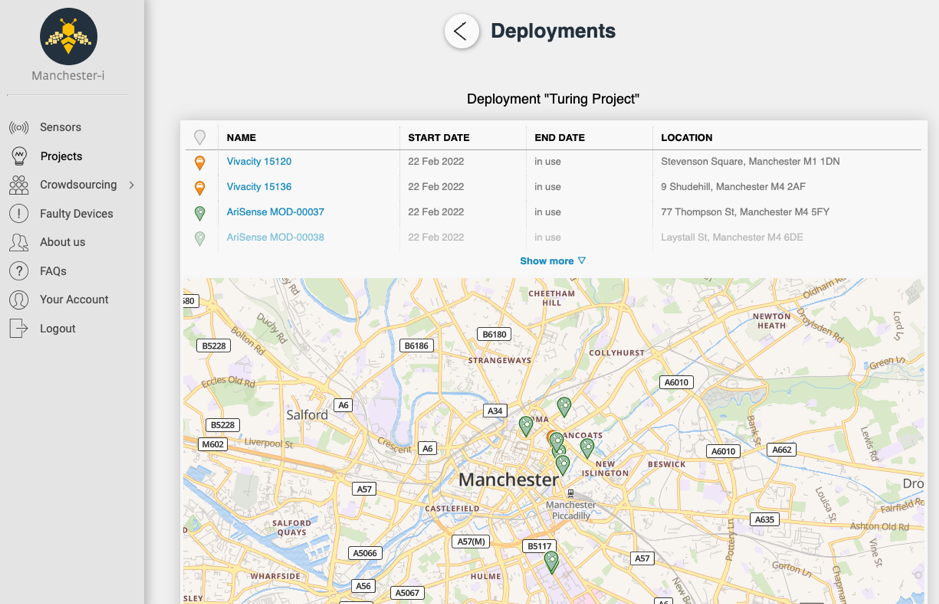
\includegraphics[width=0.95\linewidth]{Figures/manchester-i-1.png}	
	\caption{Snapshot of the new data streams now publicly available through the Manchester-i portal} \label{fig::manchesteri}
\end{figure}

%%%%%%%%%%%%%%%%%%%%%%%%%%%%%%%%%%%%%%%%%%%%%%%%%%%%%%%%%%%%%%%%%%
%%%%%%%%%%%%%%%%%%%%%%%%%%%%%%%%%%%%%%%%%%%%%%%%%%%%%%%%%%%%%%%%%%
\clearpage
\subsection{EMEP model configuration and simulation}

%%%%%%%%%%%%%%%%%%%%%%%%%%%%%%%%%%%%%%%%%%%%%%%%%%%%%%%%%%%%%%%%%%
%%%%%%%%%%%%%%%%%%%%%%%%%%%%%%%%%%%%%%%%%%%%%%%%%%%%%%%%%%%%%%%%%%

The European Monitoring and Evaluation Programme for Transboundary Long-Range Transported Air Pollutants (EMEP) model is a 3-D Eulerian chemical transport model that integrates chemical processes (such as dry deposition and washout, emissions from anthropogenic and biogenic sources, gas-phase chemical reactions) with large-scale transport processes \citep{Simpson2012}. The model version used for this study is v4.33 (201906). The EMEP model is driven by meteorological fields taken at 3-hourly intervals from the Weather Research and Forecasting (WRF) model (v4.1.3) simulations \citep{Skamarock2019}, which in turn are driven by ERA-5 global meteorological data. \\

\noindent The model setup consists of two domains. The traditional 50km resolution EMEP domain covering all of Europe (an area of 8,500 x 6,650 km) is used to create chemical boundary conditions for a second, higher resolution (3km) domain covering the majority of the British Isles (an area of 1,080 x 1,080 km). Anthropogenic emissions for the outer domain are taken from the TNO database for reporting year 2017, at a resolution of 0.1 x 0.1 degrees. This dataset is provided as a standard input for the EMEP model. For the inner domain, UK National Atmospheric Emissions Inventory (NAEI) emissions (http://naei.defra.gov.uk), for the reporting year 2016 and at a resolution of 1 x 1 km, are used for the UK, Atlantic, and North Sea regions, while TNO emissions are used for the rest of the domain (covering the Republic of Ireland, and parts of France).

\begin{figure}
	\centering
	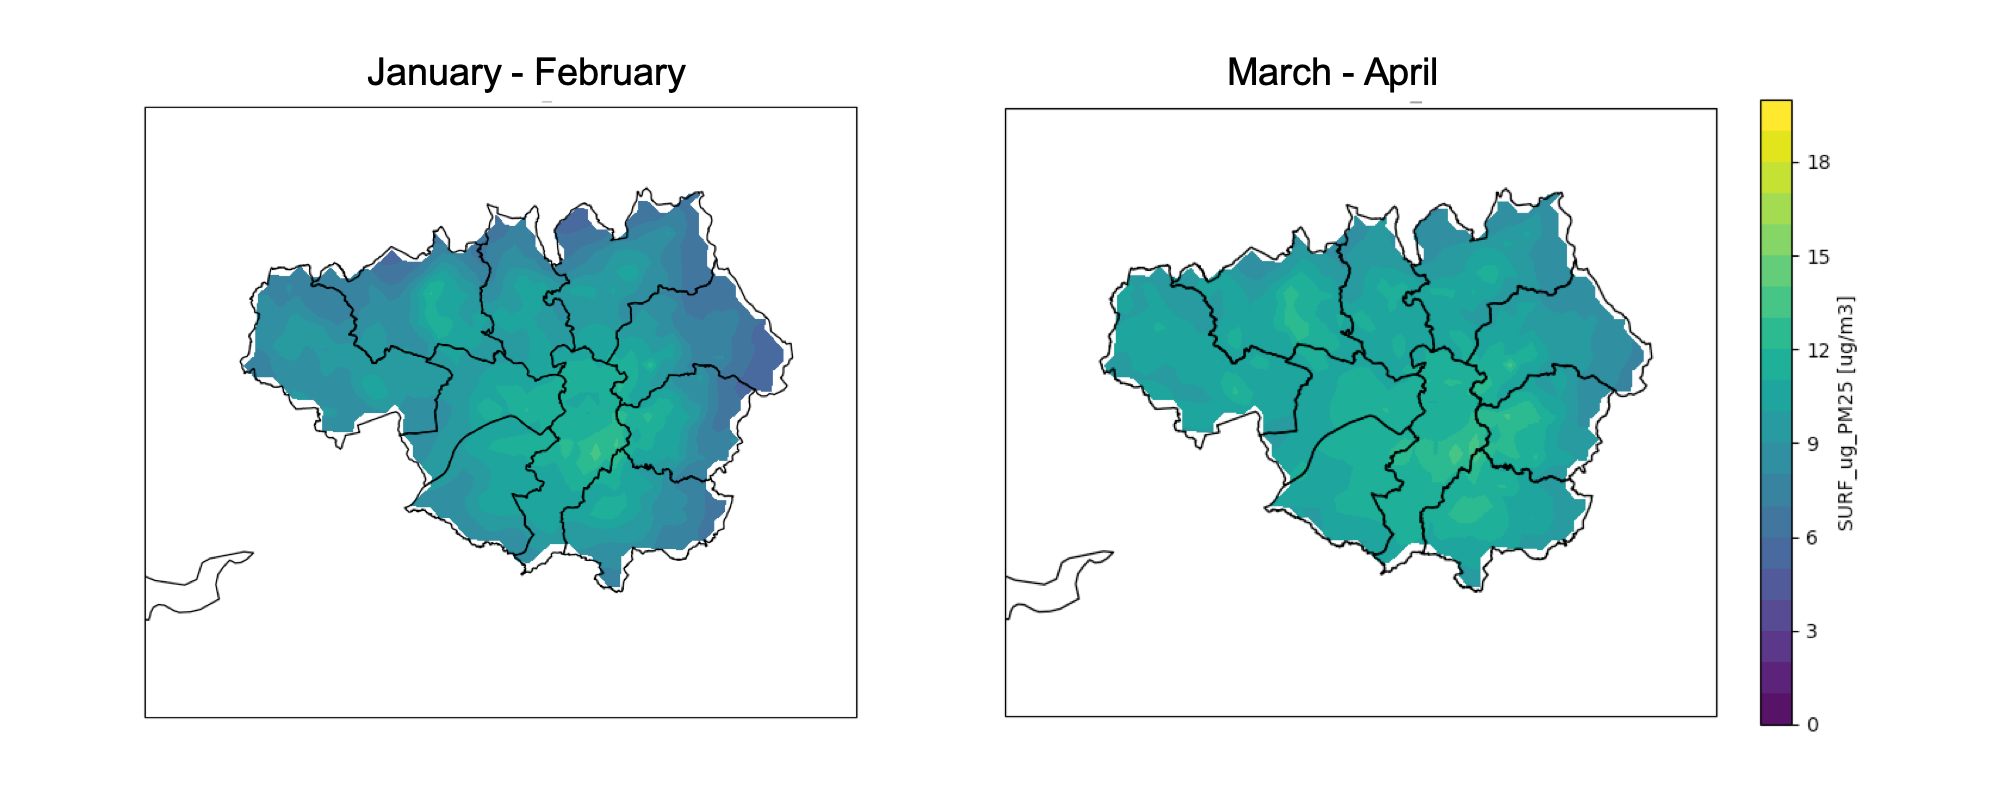
\includegraphics[width=0.95\linewidth]{Figures/EMEP.png}		
	\caption{Geospatial predictions of average PM$_{2.5}$ in Manchester from the EMEP simulations for Jan-Feb (left) and Mar-Apr (right) respectively} \label{fig::emep}
\end{figure}

%%%%%%%%%%%%%%%%%%%%%%%%%%%%%%%%%%%%%%%%%%%%%%%%%%%%%%%%%%%%%%%%%%
%%%%%%%%%%%%%%%%%%%%%%%%%%%%%%%%%%%%%%%%%%%%%%%%%%%%%%%%%%%%%%%%%%
%%%%%%%%%%%%%%%%%%%%%%%%%%%%%%%%%%%%%%%%%%%%%%%%%%%%%%%%%%%%%%%%%%
\clearpage
\section{Case study: Devon}\label{sec::casestudy1}

%%%%%%%%%%%%%%%%%%%%%%%%%%%%%%%%%%%%%%%%%%%%%%%%%%%%%%%%%%%%%%%%%%
%%%%%%%%%%%%%%%%%%%%%%%%%%%%%%%%%%%%%%%%%%%%%%%%%%%%%%%%%%%%%%%%%%
%%%%%%%%%%%%%%%%%%%%%%%%%%%%%%%%%%%%%%%%%%%%%%%%%%%%%%%%%%%%%%%%%%

\noindent The initial development of the computational implementation of DIMEX was used to investigate personal exposures for a sub-population in Devon. Devon is a county in the South-west of England, comprises ten local authorities boroughs: Exeter, East Devon, Mid Devon, North Devon, Plymouth, South Hams, Teignbridge, Torbay, Torridge and West Devon and has an estimated population of 800,000. Each local authority is further split into MSOAs, of which there are 156 in Devon. Figure \ref{fig::studyregiondvn} shows a map of Devon, split by the local authorities  and the MSOAs. \\

\begin{figure}[!hbtp]
	\centering
	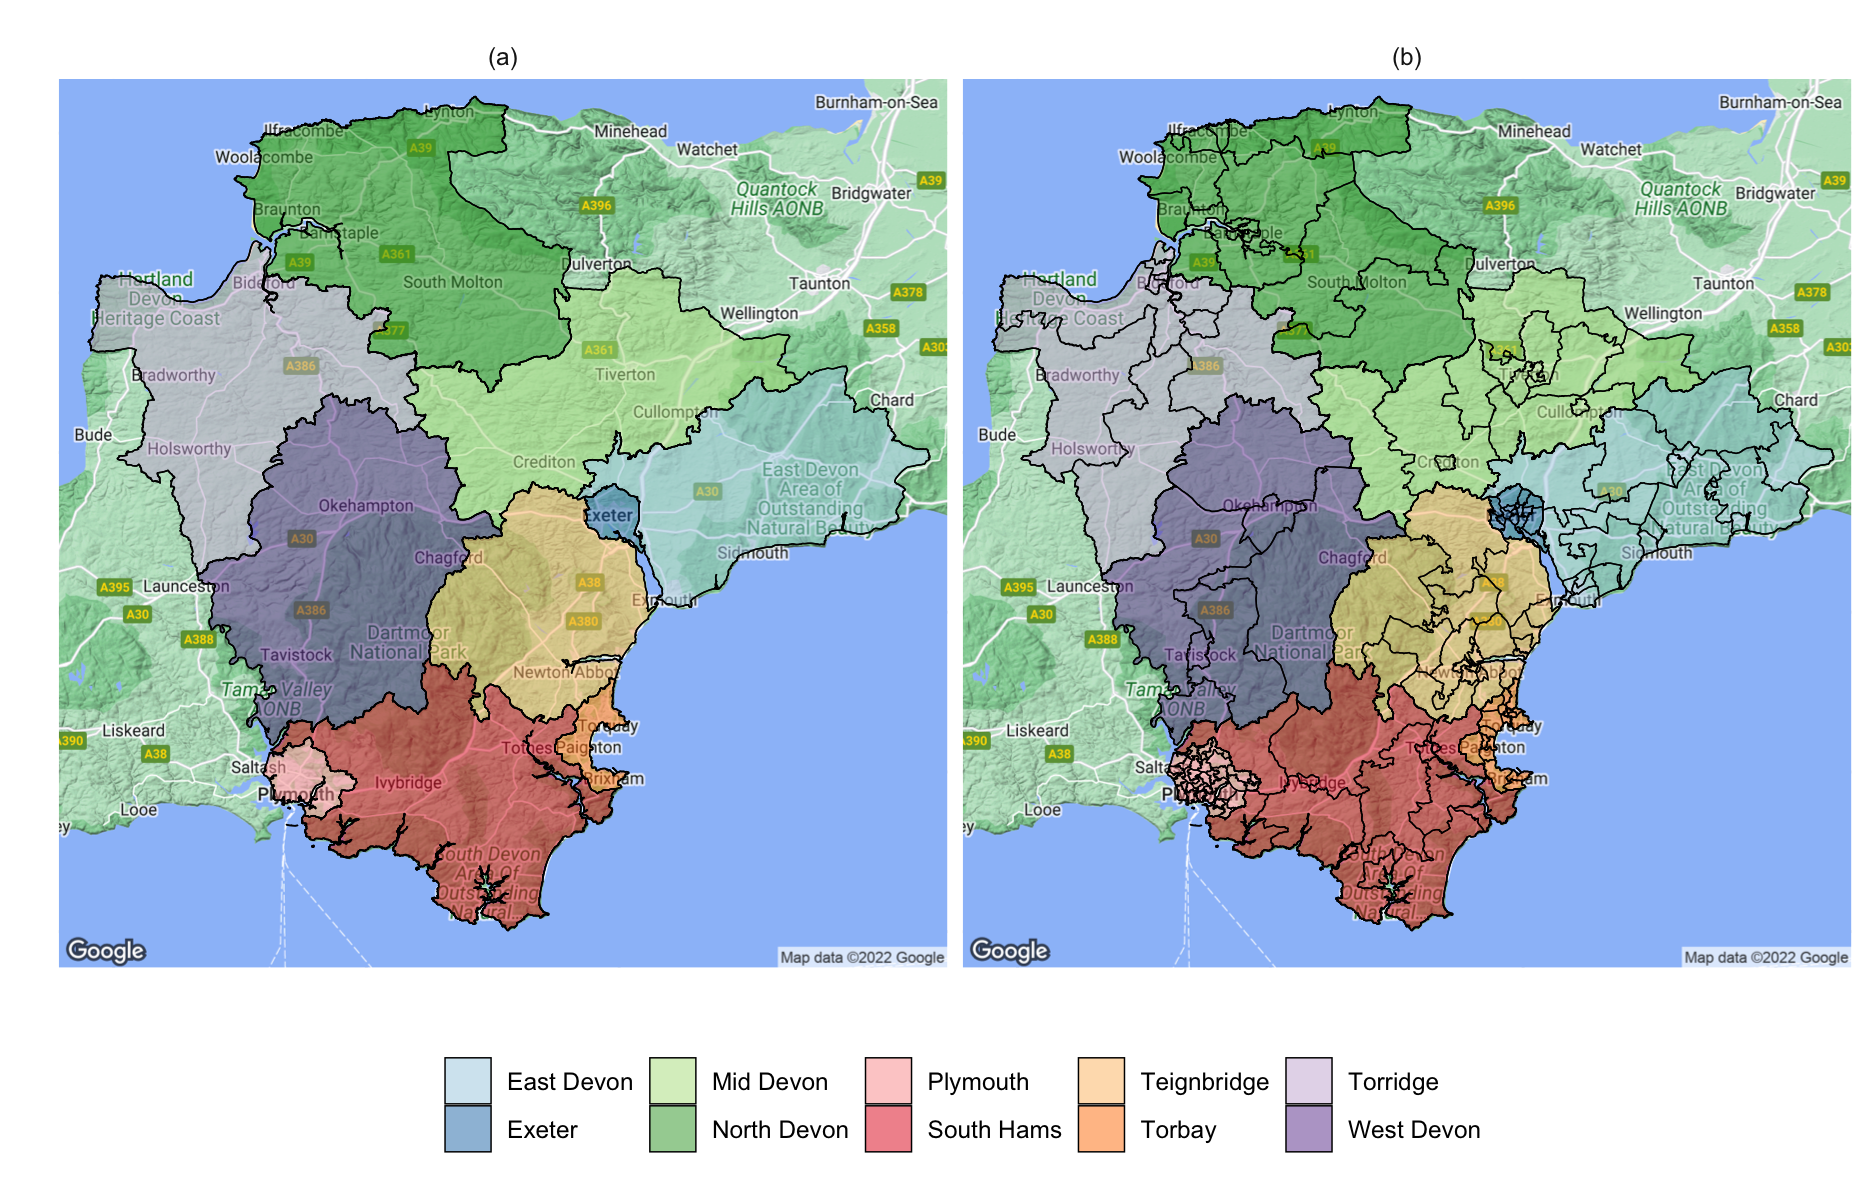
\includegraphics[width=0.9\linewidth]{Figures/Devon_GGMAP}		
	\caption{Study region of Devon, with boundaries indicating by (a) local authories and (b) MSOAs. } \label{fig::studyregiondvn}
\end{figure}
\begin{figure}[!hbtp]
	\centering
	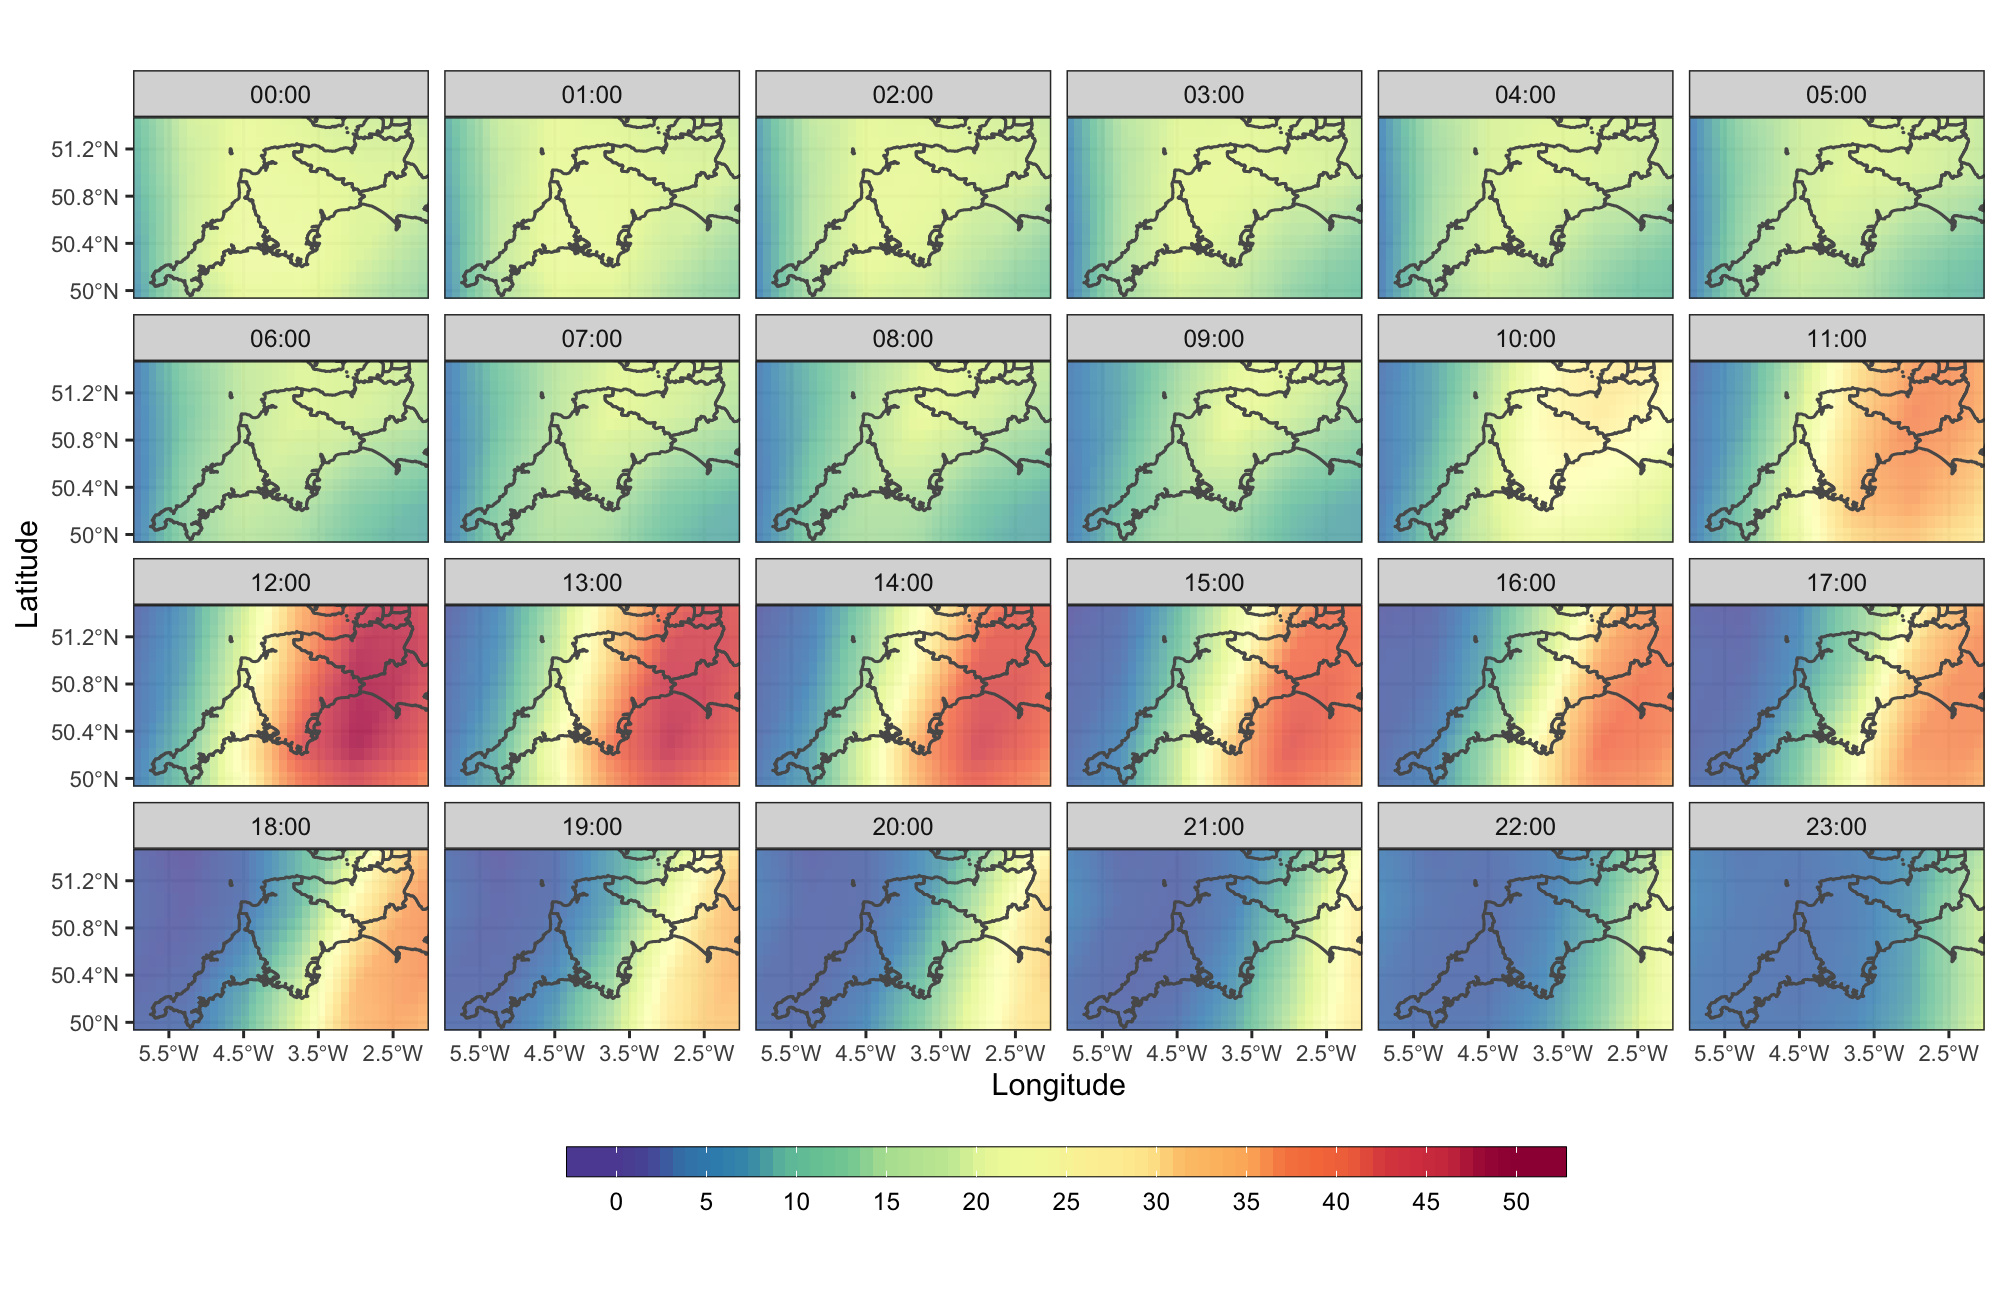
\includegraphics[width = 0.9\linewidth]{Figures/PM25_20190501}
	\caption{Estimated hourly concentrations of PM$_{2.5}$ (in $\mu$g/m$^3$) from the Copernicus Atmosphere Monitoring Service reanalysis model for the South-West of England on 1 May 2019, by grid-cell (0.1$^{o}$ $\times$ 0.1$^{o}$ resolution)}
	\label{fig::PMConc}
\end{figure}

\noindent Information on ambient concentrations of PM$_{2.5}$ for the South-West of England between 1 January 2019 to 31 December 2019 were obtained from the Copernicus Atmosphere Monitoring Service (CAMS) reanalysis model. The CAMS model produces estimates of PM$_{2.5}$ (in $\mu$g/m$^3$) on a 0.75$^{o}$ $\times$ 0.75$^{o}$ resolution grid in three-hour intervals \citep{CAMS}. Linear interpolation was used to downscale the estimates of PM$_{2.5}$ to increase the spatial resolution, from a 0.75$^{o}$$\times$0.75$^{o}$ grid to a 0.1$^{o}$$\times$0.1$^{o}$ grid, and  the temporal resolution  from three-hourly increment to hourly increments. Figure \ref{fig::PMConc} shows the hourly estimated concentrations of PM$_{2.5}$ on 1 May 2019. In 2019, the hourly estimated concentrations of PM$_{2.5}$ ranged from 0.0$\mu$g/m$^3$ to 164.9$\mu$g/m$^3$, with mean concentration of 9.6$\mu$g/m$^3$ and a median concentration of 7.9$\mu$g/m$^3$. \\

\noindent Information on temperature for the South-West of England between 1 January 2019 to 31 December 2019 were also obtained from CAMS reanalysis model. The CAMS model produces estimates of the air temperature (in Celsius) 2 metres above the surface on a 0.75$^{o}$$\times$0.75$^{o}$ resolution grid in three-hour intervals \citep{CAMS}. Linear interpolation was used to downscale the temperature estimates increasing the spatial resolution from a 0.75$^{o}$$\times$0.75$^{o}$ grid to a 0.1$^{o}$$\times$0.1$^{o}$ grid. Estimates were then aggregated over time to produce the daily average temperature for each 0.1$^{o}$$\times$0.1$^{o}$ grid-cell.  \\

\noindent DIMEX was used to estimate personal exposures of 30 females from Devon, aged 19 to 29, who are employed, work during the day and do not smoke in April and July 2019. Each individual has hourly activity sequences generated for each day of the month, and matched with the corresponding hourly estimated concentrations of PM$_{2.5}$ in each micro-environment to obtain personal exposures.  Figure \ref{fig::expme} shows the predictive distribution of the personal exposures to PM$_{2.5}$ by micro-environments (`home', `indoor not home', `outdoor' and `transport') in each month. In both months, the the lowest and highest exposures to PM$_{2.5}$ are observed in the `home' and `transport' micro-environments respectively. There are substantial differences in the potential exposures to PM$_{2.5}$ between these micro-environments with the change in exposure from being `home' and being in `transport' can be as high as 30$\mu$g/m$^3$. Exposures to PM$_{2.5}$ in the `indoor not home' micro-environment are similar in both April and July and are higher than the `home' environment. The `outdoor' micro-environment sees the biggest variation, with exposures higher than `indoor not home' in April and lower then `indoor not home' in July. The range of `outdoor' exposures is larger in April than in July, due to large spikes in the concentrations of PM in late April. \\

\noindent Figure \ref{fig::exphour} shows the predictive distribution of personal exposures to PM$_{2.5}$ by hour of the day in each month. It can be seen that the days are split into two parts: (a) 22:00 to 05:00 and (b) 06:00 to 21:00. Between 22:00 to 05:00 individuals are assumed to remain at `home', and as concentrations of PM$_{2.5}$ are the lowest of all micro-environments (See Figure \ref{fig::expme}) the exposures will be low as a result. Between 06:00 to 21:00, individuals can move between any of the micro-environments, where the estimated concentrations of PM$_{2.5}$ are higher and have a larger variability, which is again reflected in the overall exposures. \\

\begin{figure}[!hbtp]
	\centering
	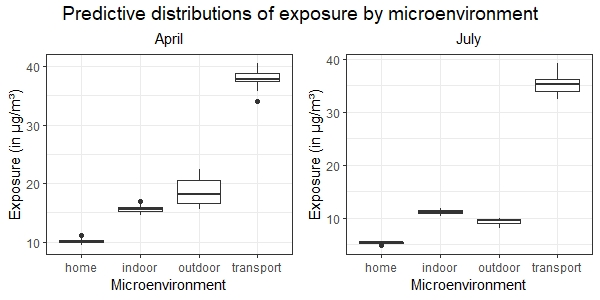
\includegraphics[width = \linewidth]{Figures/plot_ME}
	\caption{Predictive distribution of the personal exposures to PM$_{2.5}$ by micro-environments (`home', `indoor not home', `outdoor' and `transport') in April and July.}
	\label{fig::expme}
\end{figure}
\begin{figure}[!hbtp]
	\centering
	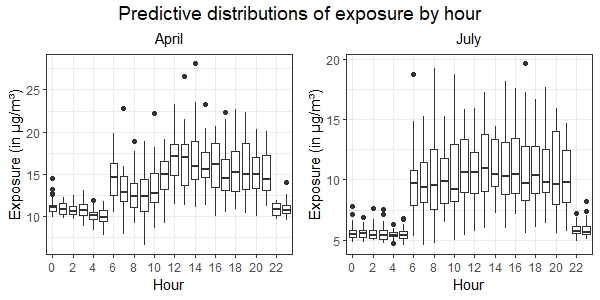
\includegraphics[width = \linewidth]{Figures/plot_hour}
	\caption{Predictive distribution of the personal exposures to PM$_{2.5}$ by hour in April and July.}
	\label{fig::exphour}
\end{figure}
\begin{figure}[!hbtp]
	\centering
	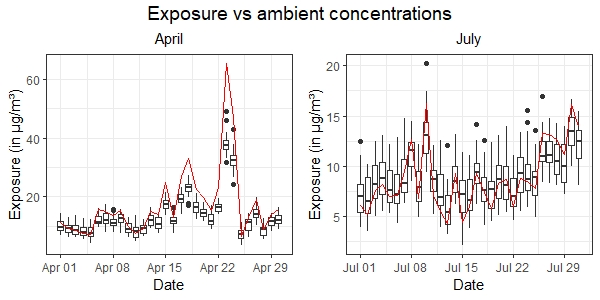
\includegraphics[width = \linewidth]{Figures/plot_ambient}
	\caption{Predictive distribution of the personal exposures to PM$_{2.5}$ by day along with the estimated ambient concentration of PM$_{2.5}$ from the CAMS reanalysis model in April and July.}
	\label{fig::expdaily}
\end{figure}

\noindent Figure \ref{fig::expdaily} shows the predictive distribution of personal exposures to PM$_{2.5}$ by day, along with the estimated ambient concentration of PM$_{2.5}$ from the CAMS reanalysis model. As expected, the daily exposures to PM$_{2.5}$ follow a similar pattern to that of the estimates of PM$_{2.5}$ from the CAMS reanalysis. In April, exposures are generally lower than the ambient concentrations of PM$_{2.5}$. This is particularly noticeable in late April where exposures are much lower than the spikes in ambient outdoor concentration estimated from CAMS. This is likely due to individuals spending most of their day in indoor micro-environments, in effect, being `protected' from high concentrations that may be experienced outdoors. The opposite can be observed in July, where exposures are higher than the estimated ambient concentrations of PM$_{2.5}$ on some days. As ambient concentrations of PM$_{2.5}$ are lower than those indoors (because of non-ambient sources of PM$_{2.5}$) these days, spending most of your time indoors may lead to higher exposure to PM$_{2.5}$. For this reason, it is important to differentiate the times that individuals spend in each micro-environment to get an accurate and representative estimate of exposure as exposures to PM$_{2.5}$ estimated solely from ambient concentrations could potentially over- or underestimate personal exposure depending on the time period of interest and the individuals behaviours. \\

\noindent Table \ref{tab::exceedances} shows the estimated a number of times the daily exposure to PM$_{2.5}$ (of the sub-population) and the ambient concentrations of PM$_{2.5}$ from the CAMS reanalysis model exceeded air quality standards, as defined by the Daily Air Quality Index (DAQI). The DAQI classifies indices 1 to 3 (0 to 35$\mu$g/m$^3$) as low, indices 4 to 6 (35 to 53$\mu$g/m$^3$) as moderate, indices 7-9 (53 to 70$\mu$g/m$^3$) as high and index 10 (over 70$\mu$g/m$^3$) as very high \citep{DEFRA2020}. 

\begin{table}[t]
	\centering 
	\caption{Estimated number of times the daily exposure to PM$_{2.5}$ (of the sub-population) and the ambient concentrations of PM$_{2.5}$ from the CAMS reanalysis model exceeded air quality standards, defined by the Daily Air Quality Index (DAQI). Brackets indicate }
	\begin{tabular}{c c c c c}
		\hline \hline 
		          & \multicolumn{2}{c}{April} & \multicolumn{2}{c}{July} \\
		\cmidrule(lr){2-3}
		\cmidrule(lr){4-5}
		Threshold & Personal Exposure & Ambient & Personal Exposure & Ambient \\
		\hline
		11 & 17.2 (3.68) & 21 & 6.9 (3.15) & 8 \\
		23 &  2.6 (0.25) &  6 & 0          & 0 \\
		35 &  0.9 (0.28) &  2 & 0          & 0 \\
		41 &  0.2 (0.15) &  2 & 0          & 0 \\
		47 & 0.03 (0.03) &  1 & 0          & 0 \\
		53 & 0           &  1 & 0          & 0 \\
		58 & 0           &  1 & 0          & 0 \\
		64 & 0           &  1 & 0          & 0 \\
		70 & 0           &  0 & 0          & 0 \\ 
		\hline \hline
	\end{tabular}	
	\label{tab::exceedances}
\end{table}

%%%%%%%%%%%%%%%%%%%%%%%%%%%%%%%%%%%%%%%%%%%%%%%%%%%%%%%%%%%%%%%%%%
%%%%%%%%%%%%%%%%%%%%%%%%%%%%%%%%%%%%%%%%%%%%%%%%%%%%%%%%%%%%%%%%%%
%%%%%%%%%%%%%%%%%%%%%%%%%%%%%%%%%%%%%%%%%%%%%%%%%%%%%%%%%%%%%%%%%%
\clearpage
\section{Case study: Greater Manchester}\label{sec::casestudy2}

%%%%%%%%%%%%%%%%%%%%%%%%%%%%%%%%%%%%%%%%%%%%%%%%%%%%%%%%%%%%%%%%%%
%%%%%%%%%%%%%%%%%%%%%%%%%%%%%%%%%%%%%%%%%%%%%%%%%%%%%%%%%%%%%%%%%%
%%%%%%%%%%%%%%%%%%%%%%%%%%%%%%%%%%%%%%%%%%%%%%%%%%%%%%%%%%%%%%%%%%

\noindent Air pollution is a significant risk to public health and is the leading environmental risk for adverse population health outcomes globally \cite{rep_2017,who_2016,RCP_rep_2016,Par_report}. A number of different air pollutants have been associated with adverse health effects, including fine particulate matter, nitrogen dioxide and ozone. Many studies have implicated fine particulate  air pollution as contributing to the incidence and severity of respiratory disease \citep{pope:95}.  Epidemiological studies have consistently reported associations between a variety of pollutants and both mortality and morbidity, \citep{laden_2000,dominici2000measurement,dominici_2002}. Many epidemiological research studies across the world have shown that exposure to poor air quality impacts on people's health. \\

\noindent Current EU statutory limits state that annual average concentrations of NO$_{2}$ and PM$_{2.5}$ should not exceed 40 $\mu$g/m$^{3}$ and 25 $\mu$g/m$^{3}$ respectively \citep{EEAAQGs}. Designed to protect the public from the adverse health effects of air pollution, the World Health Organisation (WHO) Air Quality Guidelines (AQG),  on PM$_{2.5}$, were much lower than the EU statutory limits for PM$_{2.5}$, stating annual averages should not exceed 10 $\mu$g/m$^{3}$ \citep{world2006air}. In 2021, the WHO re-issued notably reduced air quality guidelines for annual average PM$_{2.5}$ from 10 $\mu$g/m$^{3}$ to 5 $\mu$g/m$^{3}$ \citep{weltgesundheitsorganisation2021global}, reflecting the increasing evidence of adverse health effects of air pollution at lower levels.\\

\noindent As described in the Section 4, exposure to air pollution depends on the activity and time use profile of each individual and the micro-environments in which they are carried out (at home, outside, in-work) \citep{borghi2021estimation}. In turn, an individuals activity and time use depends on their demographic and socioeconomic characteristics. To date, epidemiological research to date has focused primarily on the impact of ambient pollution on health outcomes, despite time use data demonstrating that Europeans now spend 89 percent of time indoors \citep{mcgrath2017pm}, with approximately 70 percent of this time in the home environment \citep{klepeis2001national, schweizer2007indoor}, increasing to 90 percent in vulnerable populations such as the very young, the infirm and elderly \citep{spalt2016time, Torfs2008}. Gender differences in activities and time use, mean that women, spending a higher percentage of their time in the home environment, have higher levels of exposure to air pollutants within the residential environment \citep{borghi2021estimation}. \\    

\noindent Traditional epidemiological risk models for air pollution have focused on ambient air pollution and are based on measured, or modelled, concentrations acting as a proxy for the exposures experienced by a population. These exposures are then aggregated to align to the level of aggregation for which health outcomes are available, typically at much higher spatial resolutions than the air pollution data. In turn, whilst the health data may be broken down by sex or broad age categories, exposure data is typically measured for a place, rather than for an individual. At high spatial resolutions and with limited demographic breakdowns, this resulting data is devoid of the necessary detail to conduct meaningful health impact assessments. In response, a key outcome for DIMEX-UK was a data framework that incorporated the outputs from the personal exposure model with individual level data for meaningful health impact assessment in order to quantify the health impact of air pollution in different micro-environments by different demographic and socioeconomic based on each groups activity and time-use profile. \\

\noindent Here we demonstrate the ability of DIMEX-UK to explore differences in time activities and exposures for different population groups within Greater Manchester. We further demonstrate the ability of DIMEX-UK to examine the impact of proposed air quality strategies, across different spatial scales and different population groups under the newly revised WHO guidelines for PM$_{2.5}$. The study region is the Greater Manchester (GM) area, a combined metropolitan authority in North-west of England. GM comprises ten metropolitan boroughs: Bolton, Bury, Manchester, Oldham, Rochdale, Salford, Stockport, Tameside, Trafford and Wigan and has an estimated population of 2.8 million. Each metropolitan borough is further split into a smaller census geography called Middle Layer Super Output Area (MSOA) in which each area represents a mean population in the order of 7,200 individuals. Figure \ref{fig::studyregion} shows a map of the study area, split by the metropolitan boroughs and the MSOAs. \\

\begin{figure}[!hbtp]
	\centering
	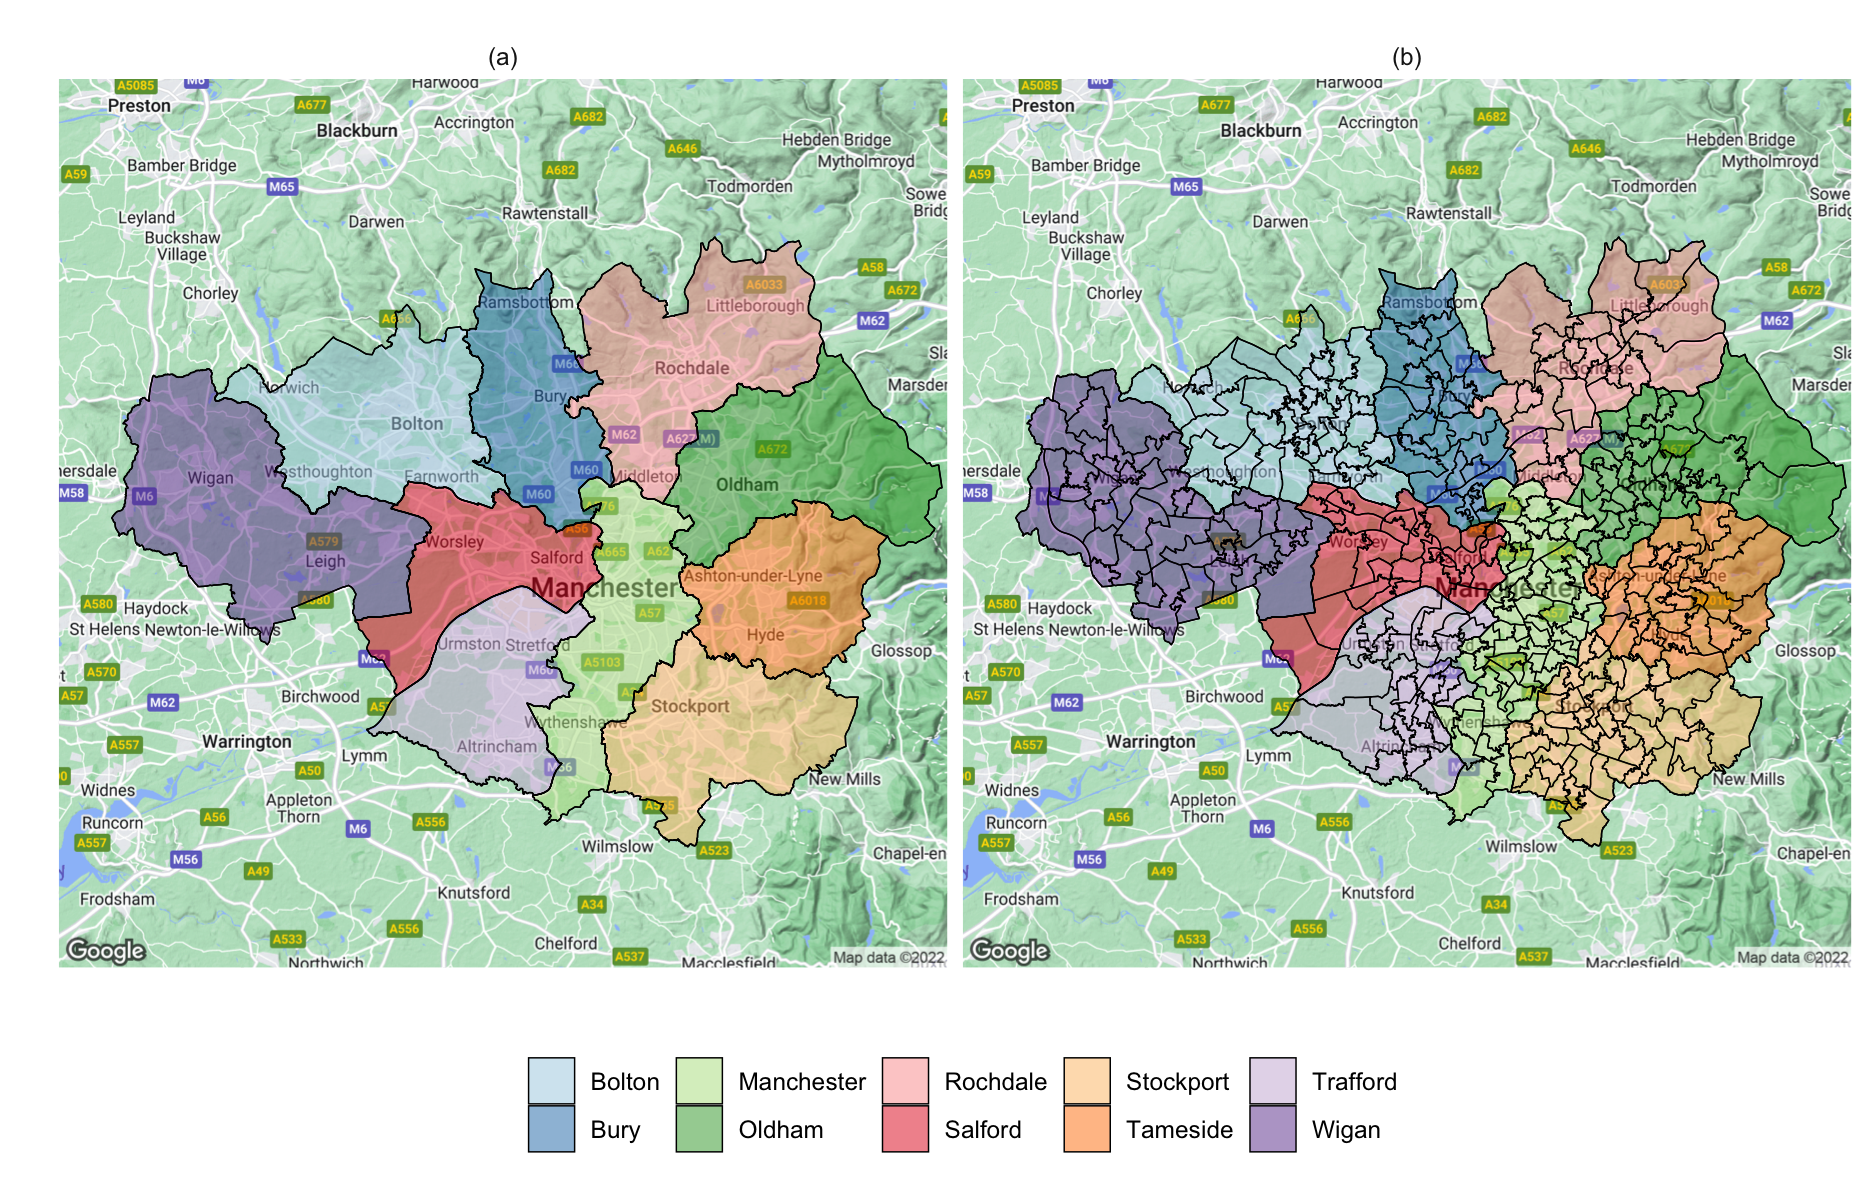
\includegraphics[width=0.95\linewidth]{Figures/Manchester_GGMAP}		
	\caption{Study region of Greater Manchester split by (a) metropolitan boroughs and (b) MSOAs. } \label{fig::studyregion}
\end{figure}

\noindent Figure \ref{fig::TimeUse_AgeGr_sex_Manchester} shows the proportion of time spent in different micro-environments by age and gender. It demonstrates the clear differences in the time spent at indoors versus outdoors across both gender and age groups. Regarding time spent in indoor environments, we further see large differences between time spent in-doors-at-home versus indoor-not-at-home  (i.e. workplace) for non-retirement age adults, with females spending more time at home (than males) for age groups 18-29, 30-44 and 45-59. \\

\begin{figure}[!hbtp]
	\centering
	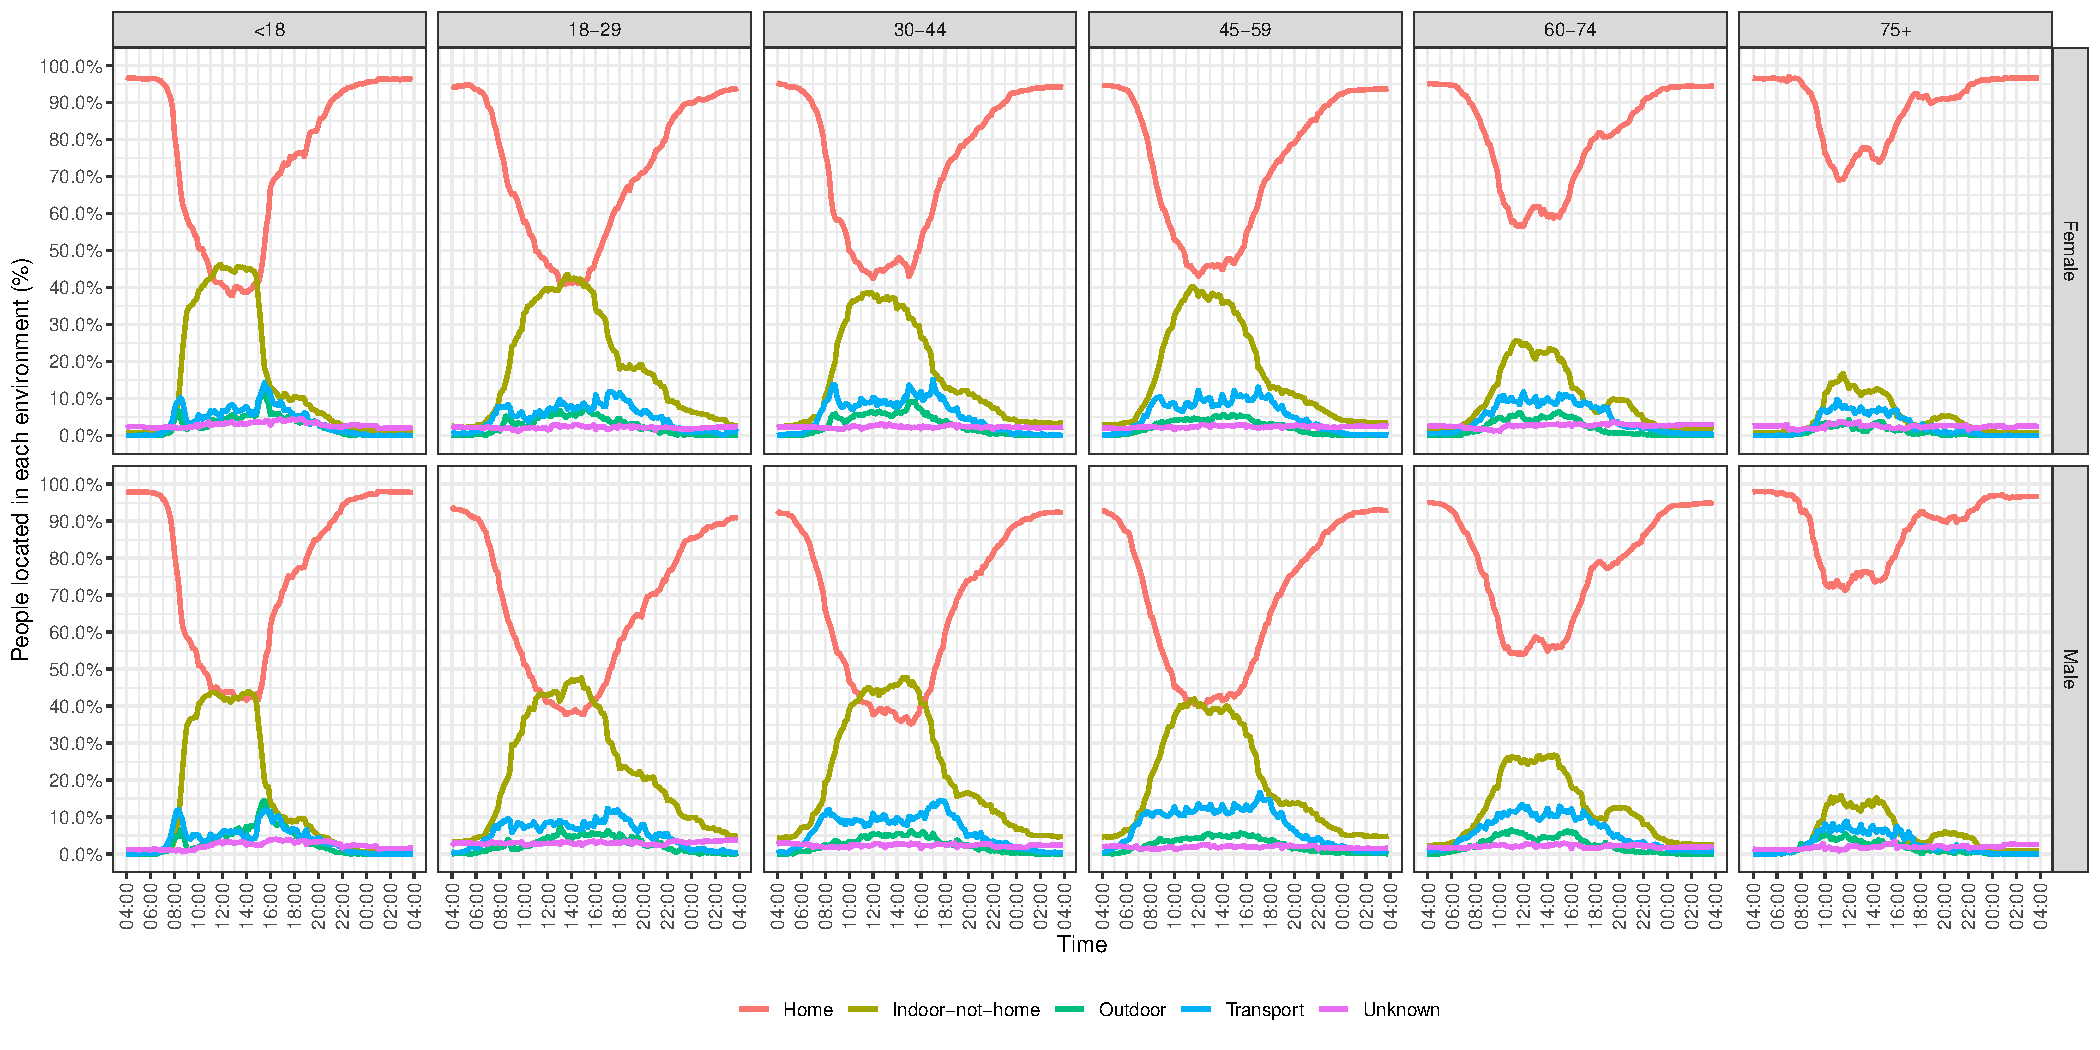
\includegraphics[width=0.95\linewidth]{Figures/TimeUse_AgeGr_sex}		
	\caption{Proportion of time spent by simulated individuals from Greater Manchester within different micro-environments (Home, Indoor-not-home, Outdoor, Transport and Unknown locations), by age and gender. } \label{fig::TimeUse_AgeGr_sex_Manchester}
\end{figure}

\noindent The following analyses demonstrate how the differing amounts of time spent in different micro-environments across different population groups affect personal exposures to air pollution. DIMEX was implemented using two different methods for providing information on ambient concentrations:

\begin{enumerate}
\item  Using measurements from the three AURN monitoring locations within the study area together with an additional six sites from the LTN for July 2021
\item  Using modelled outputs from EMEP for January - March 2021
\end{enumerate}

\noindent In each set of analyses, the results are based on a sample of 34,600 individuals within Greater Manchester (100 from each of the 346 MSOAs in the study area). The relationship between the average ambient concentrations and the personal exposures were modelled using  least-squared regression, stratified by age group and gender. The coefficients corresponding to the slopes in each of the panels representing the results from each gender-age combination can be found in Table \ref{tab::slopes}. \\

\noindent Figures \ref{fig::Fig1a} and \ref{fig::Fig1b} show the difference between estimated personal exposures and ambient concentrations using the two sources of data on ambient concentrations (measured and modelled, as described above). The Figures demonstrate the importance of indoor micro-environments as an exposure pathway for both sexes and all ages. From a demographic perspective, the difference is particularly marked for the youngest and oldest age groups, reflecting the increased proportion of time spent indoors by these population groups. \\

\begin{figure}[t]
	\centering
	\includegraphics[width=0.95\linewidth]{Figures/Fig3b}		
	\caption{Maps of (a) estimated average personal exposures to PM$_{2.5}$, (b) modelled ambient concentrations (from EMEP) and (c) Differences between daily estimated personal exposures to PM$_{2.5}$ with modelled ambient concentrations (from EMEP). Results are presented for January - March 2021.} \label{fig::Fig3b}
\end{figure}

\noindent Spatially, the differences between estimated personal exposures and ambient concentrations can seen in Figure \ref{fig::Fig3b} which maps the spatial distribution of (a) estimated personal exposures using DIMEX with the outputs from EMEP for January  - March 2022; (b) modelled ambient concentrations (from EMEP); and (c) the differences between both.\\

\begin{table}
    \centering
    \caption{Slopes obtained when fitting a least-squared regression line to estimated personal exposures and ambient concentrations (using DIMEX with measured and modelled ambient concentrations for July 2021 and January to March 2021 respectively, see text for details). Results are by gender and age group.} \label{tab::slopes}
    \begin{tabular}{l c ccc}
        \hline \hline \\[-8pt]
         & \multicolumn{2}{c}{\textbf{Measured ambient concentrations}} & \multicolumn{2}{c}{\textbf{Modelled ambient concentrations}} \\
          \cmidrule(lr){2-3}  \cmidrule(lr){4-5}\\[-10pt]
         & \textbf{Female} & \textbf{Male} & \textbf{Female} & \textbf{Male} \\
         \hline\\[-8pt]
        <16   & 0.41 & 0.41 & 0.53 & 0.53\\
        16-29 & 0.44 & 0.42 & 0.56 & 0.42\\
        30-44 & 0.40 & 0.41 & 0.48 & 0.53\\
        45-59 & 0.41 & 0.40 & 0.52 & 0.47\\
        60-74 & 0.40 & 0.40 & 0.50 & 0.51\\
        75+   & 0.38 & 0.37 & 0.51 & 0.53\\[3pt]
        \hline \hline
    \end{tabular}
\end{table}

\noindent Figures \ref{fig::Fig2a} and \ref{fig::Fig2b} show comparisons using times series plots of estimated personal exposures and ambient concentrations, with Figures \ref{fig::Fig2a_diff} and \ref{fig::Fig2b_diff} showing the corresponding differences over time. Again, it can be seen that personal exposures to PM$_{2.5}$ are generally lower than the ambient concentrations.   \\

\noindent Figures \ref{fig::Fig4a_AgeGr_Sex}--\ref{fig::Fig4b_nssec5} show the distributions of personal exposure estimates, for each age-gender combination and social-economic classification. The large variability in exposure across the different population groups can  be seen, with some individuals being exposed to levels of PM$_{2.5}$ substantially above the mean/median values that would commonly be used as summary measures. 

\noindent The data from DIMEX-UK demonstrates the importance of indoor micro-environments, particularly residential air quality, as an important exposure route that requires increased policy attention. To date guidelines on air quality with regard to health outcomes have focused solely on ambient pollution. These results demonstrate the need to develop air quality guidelines for all micro-environments to tackle the role of air quality on public health outcomes \citep{sharpe2018making} .\\

\noindent As noted, a powerful feature of DIMEX-UK is its ability to examine the impact of proposed air quality strategies, across different spatial scales and different population groups. To demonstrate this ability, DIMEX-UK was run with all  ambient concentrations across the study area  reduced to the recently updated WHO air quality guideline of 5 $\mu$g/m$^{3}$. Here we note that in some areas this might actually result in a small increase in concentrations. The results of this experiment can be seen in Figure \ref{fig::Fig5b_AgeGr_Sex}. Following these new guidelines would result in an mean (estimated) reduction in personal exposures between 2.7 and 3.1 $\mu$g/m$^{3}$, with a median reduction between 1.8 and 2.0 $\mu$g/m$^{3}$.


\newpage 
\begin{figure}[!hbtp]
	\centering
	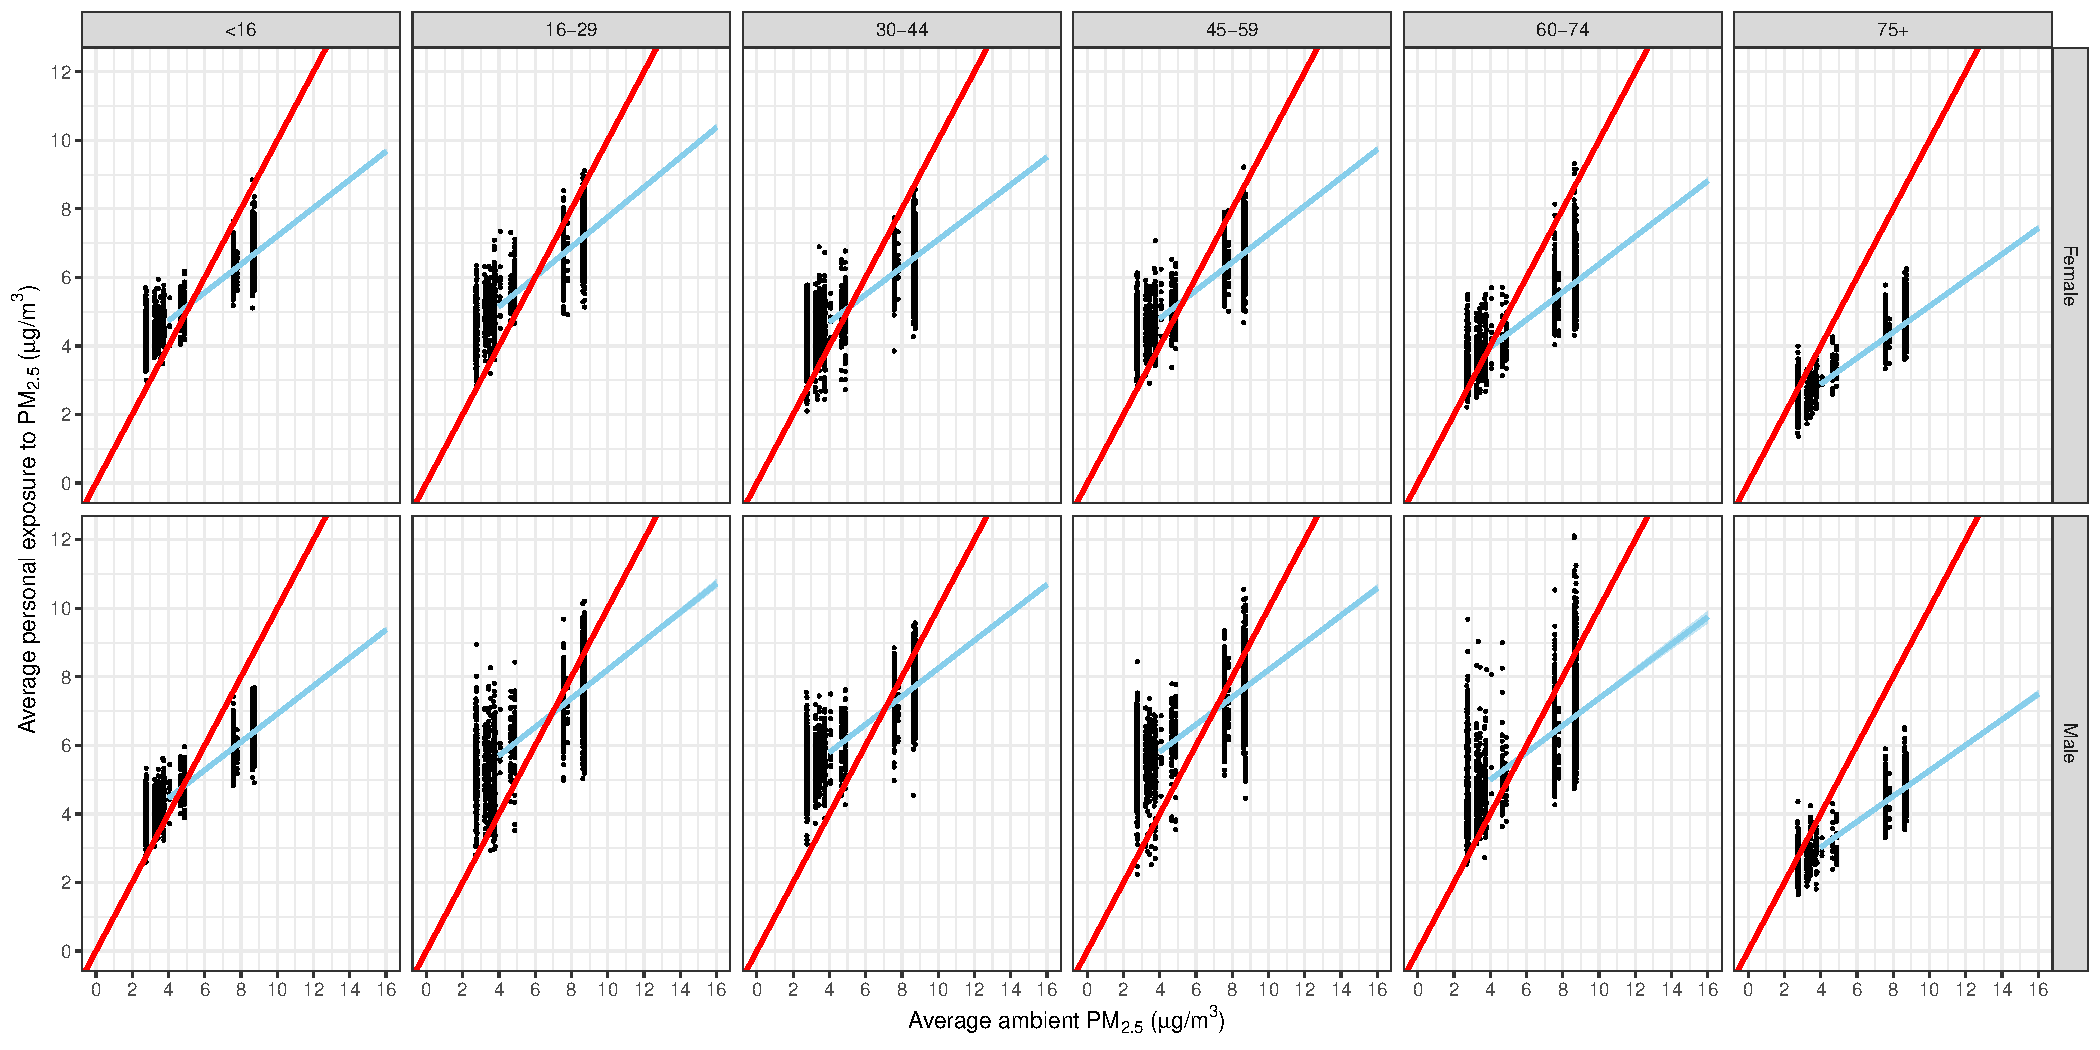
\includegraphics[width=\linewidth]{Figures/Fig1a}		
	\caption{Comparison of estimated personal exposures to PM$_{2.5}$ with ambient concentrations from measurements (from AURN and LTN, see text for details). Results are presented for July 2021, by age and gender. The red lines denote a 1:1 relationship (the idenity line), with the light blue lines showing the results of fitting least-squared regression to each age-gender combination.} \label{fig::Fig1a}
\end{figure}

\begin{figure}[!hbtp]
	\centering
	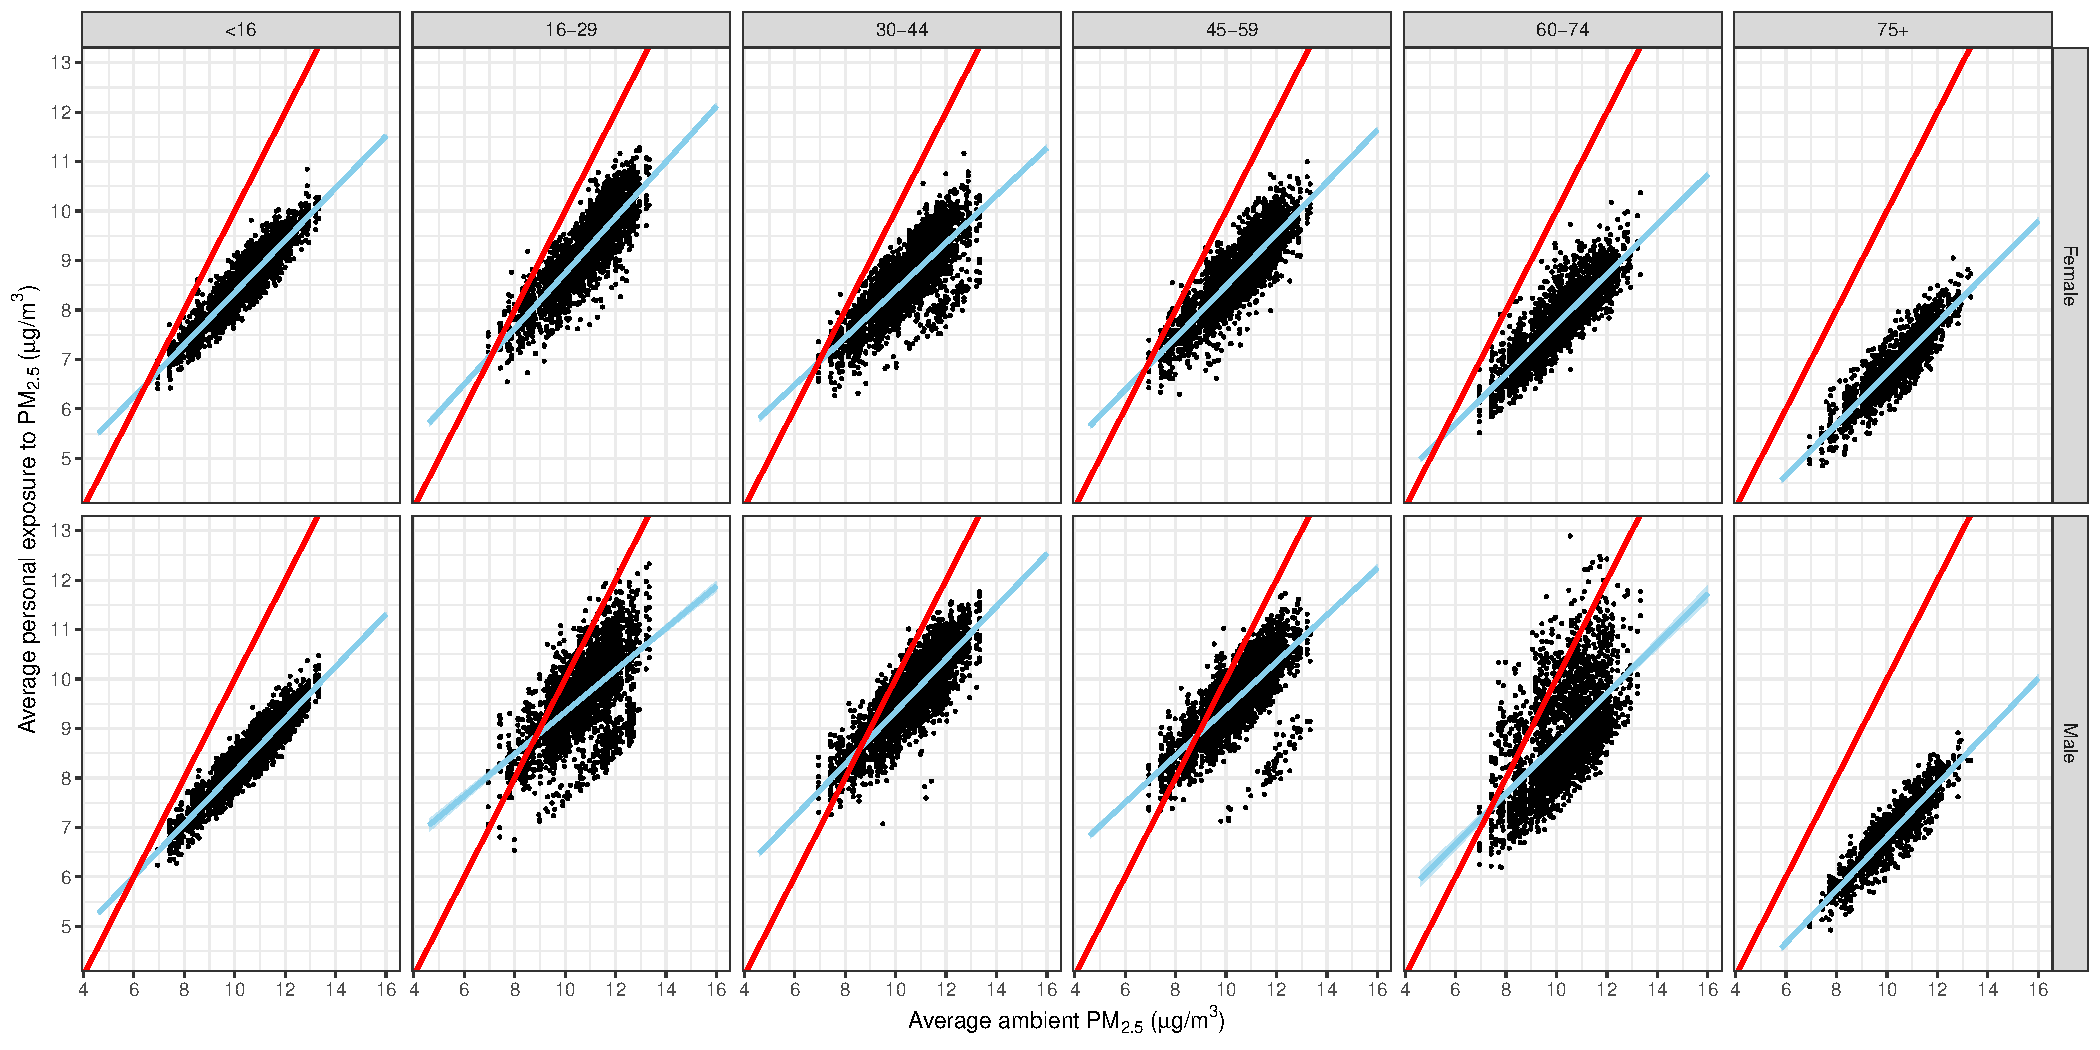
\includegraphics[width=\linewidth]{Figures/Fig1b}		
	\caption{Comparison of estimated personal exposures to PM$_{2.5}$ with modelled ambient concentrations (from EMEP), see text for details). Results are presented for January - March 2021, by age and gender. The red lines denote a 1:1 relationship (the idenity line), with the light blue lines showing the results of fitting least-squared regression to each age-gender combination.} \label{fig::Fig1b}
\end{figure}

\begin{figure}[!hbtp]
	\centering
	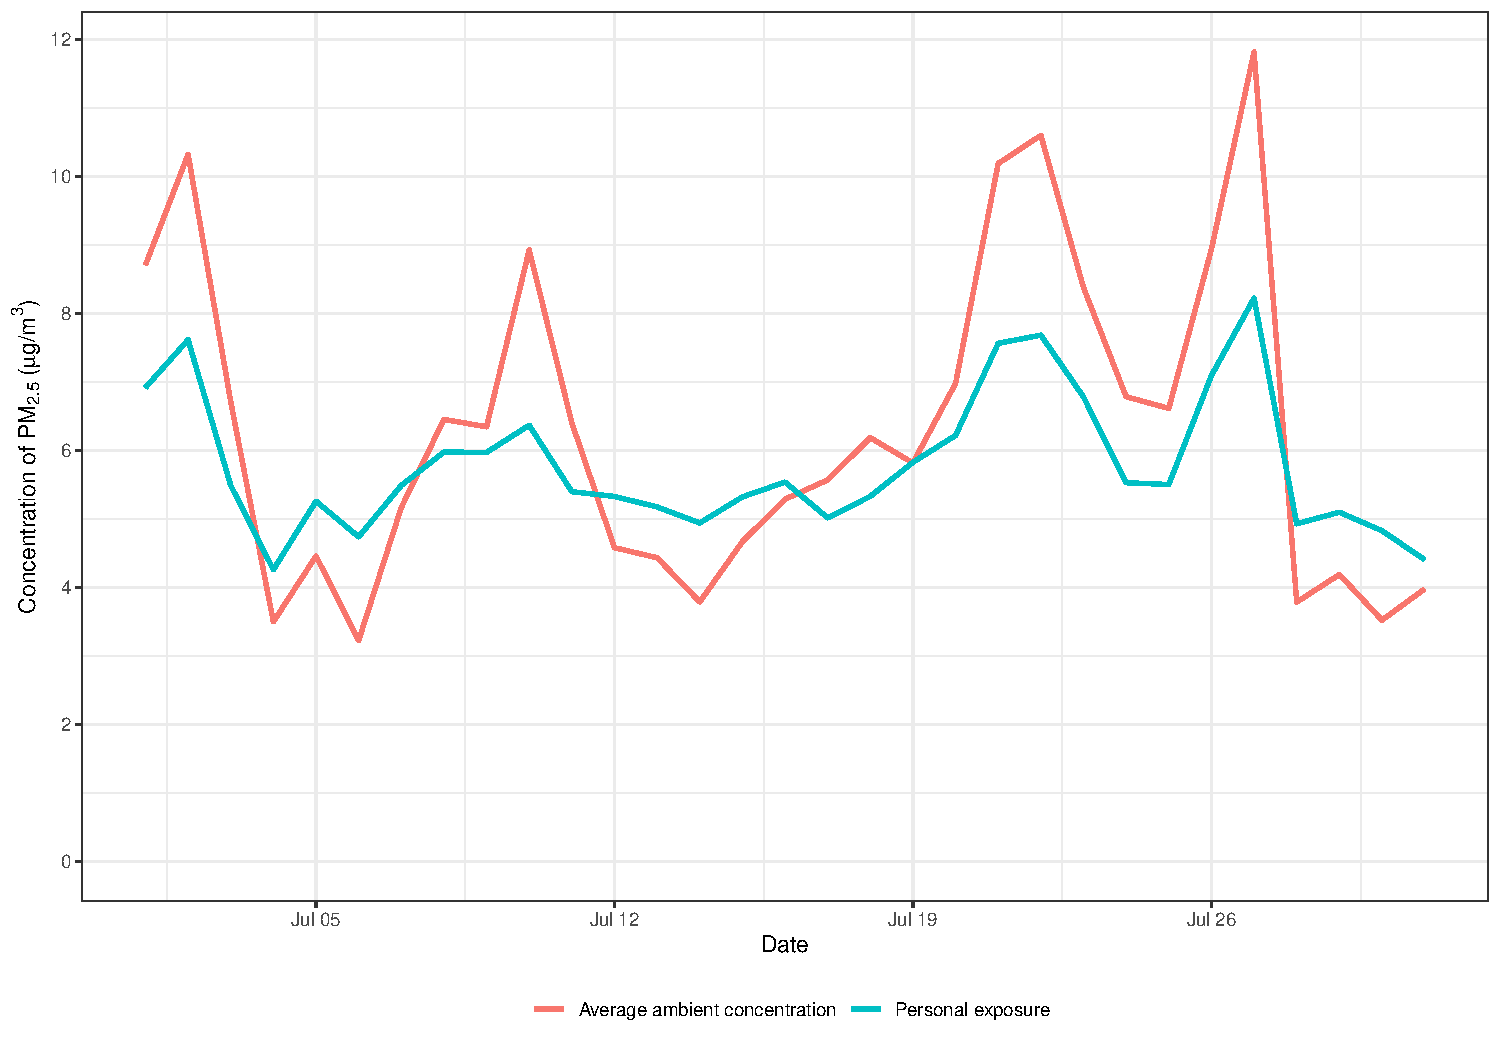
\includegraphics[width=0.85\linewidth]{Figures/Fig2a}		
	\caption{Comparison of daily estimated personal exposures to PM$_{2.5}$ with ambient concentrations from measurements (from AURN and LTN, see text for details) for July 2021} \label{fig::Fig2a}
\end{figure}
\begin{figure}[!hbtp]
	\centering
	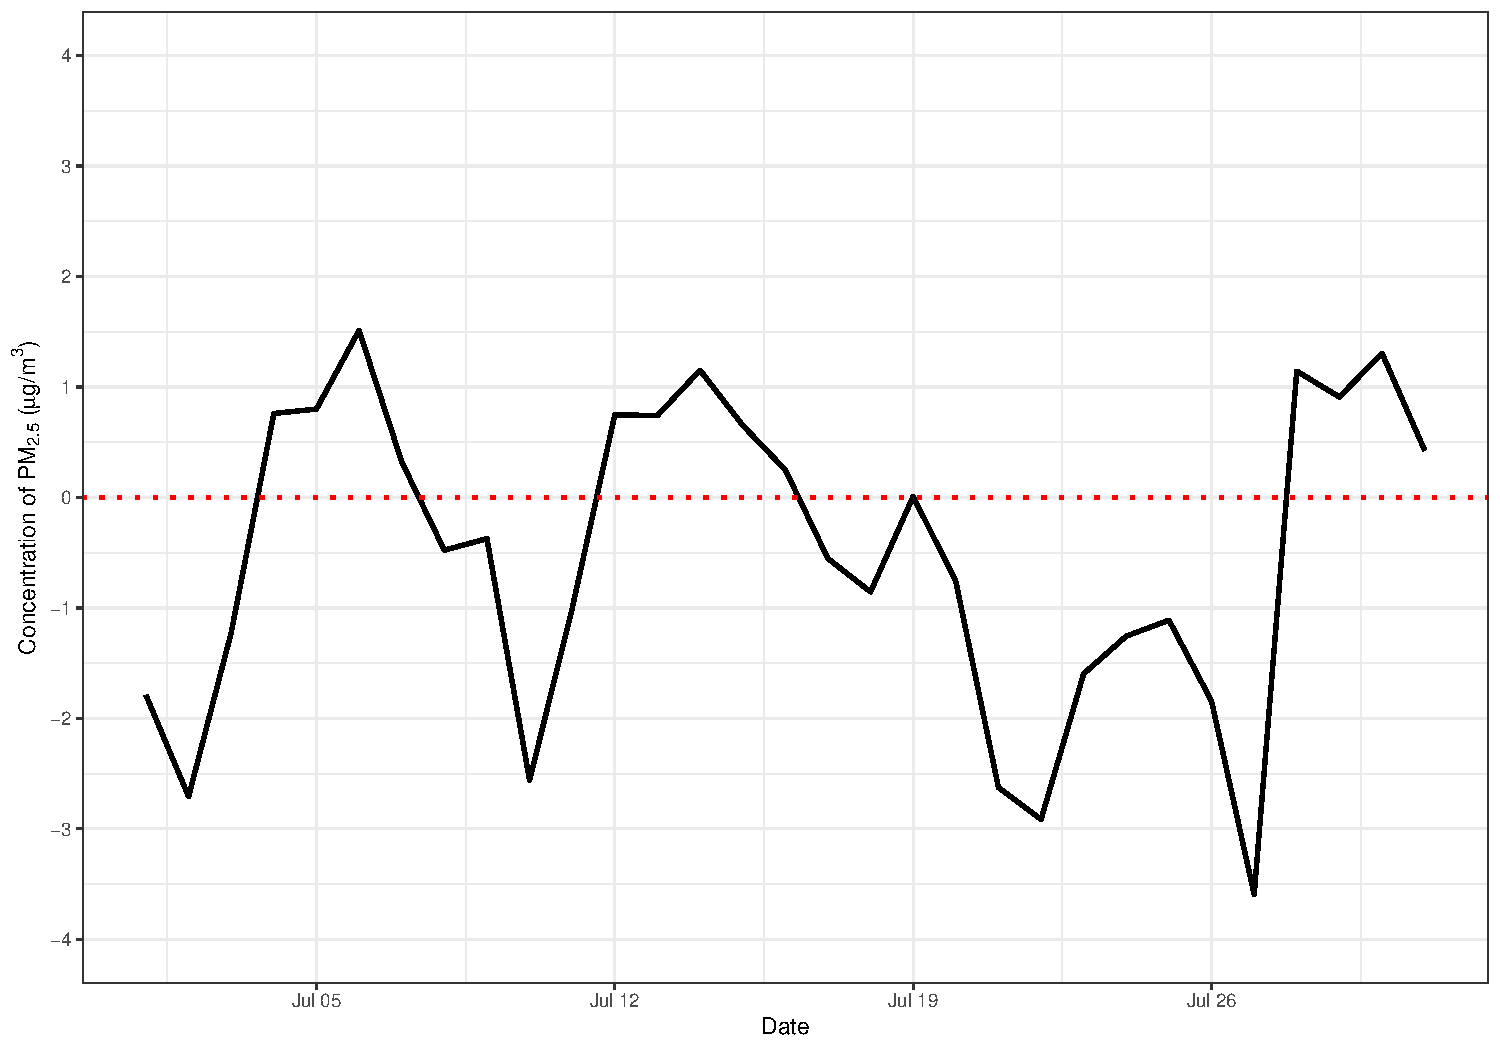
\includegraphics[width=0.85\linewidth]{Figures/Fig2a_diff}		
	\caption{Differences between daily estimated personal exposures to PM$_{2.5}$ with ambient concentrations from measurements (from AURN and LTN, see text for details) for July 2021. The dotted red line denotes a difference of zero betwen the two series of data. } \label{fig::Fig2a_diff}
\end{figure}

\begin{figure}[!hbtp]
	\centering
	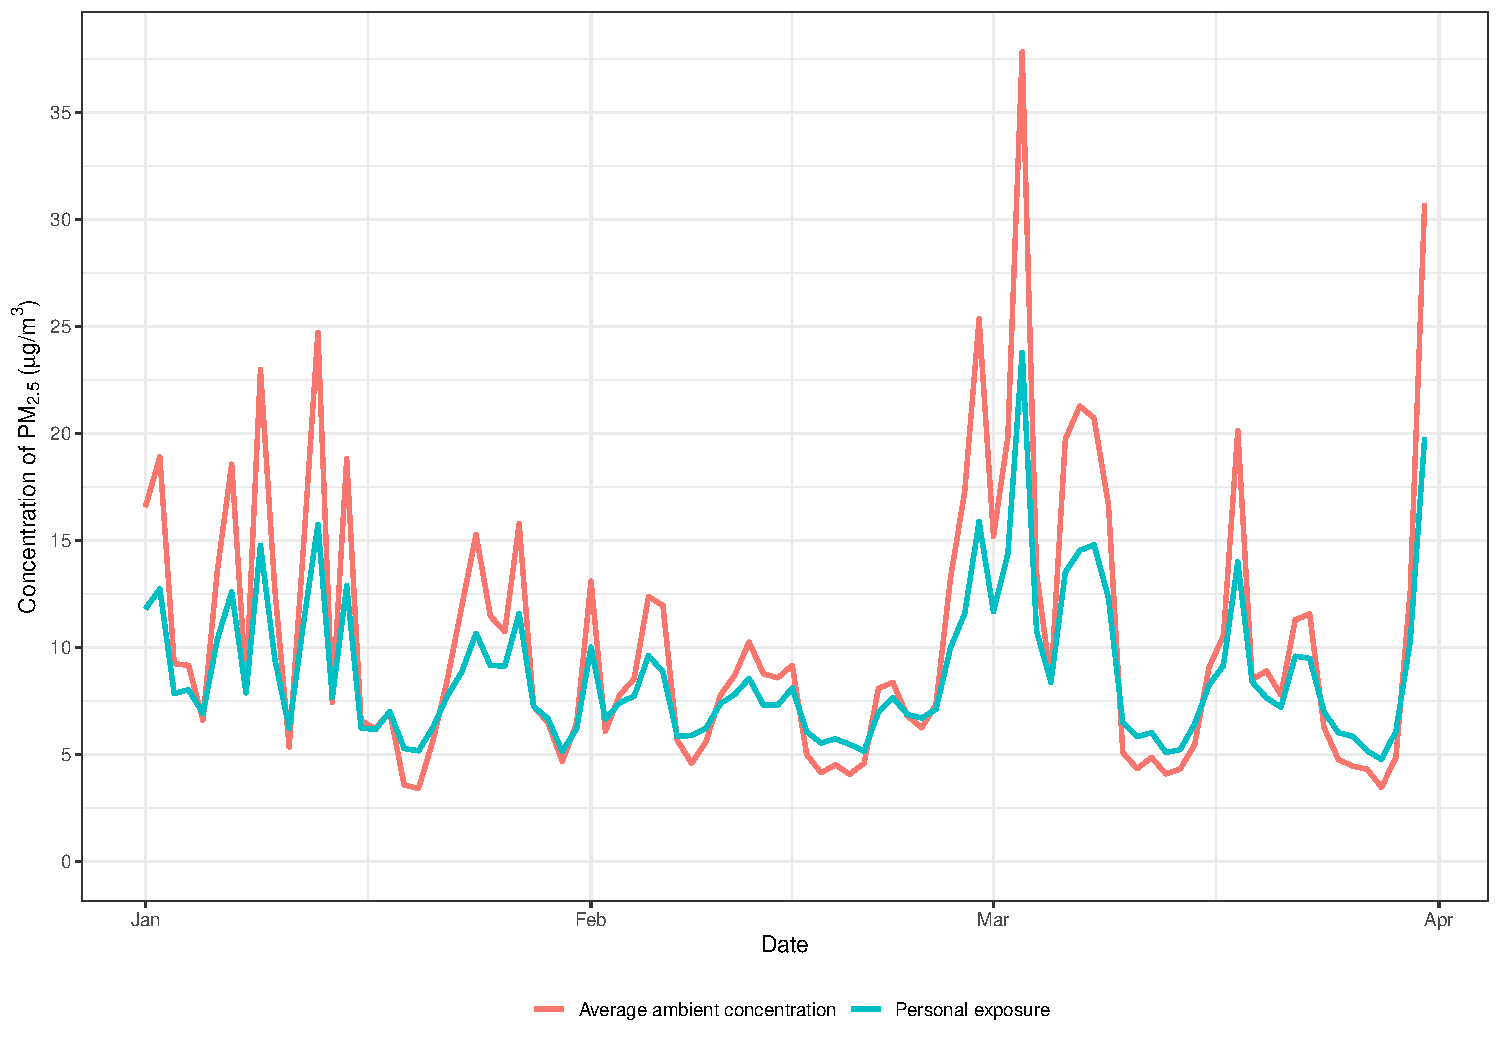
\includegraphics[width=0.85\linewidth]{Figures/Fig2b}		
	\caption{Comparison of daily estimated personal exposures to PM$_{2.5}$ with modelled ambient concentrations (from EMEP), see text for details). Results are presented for January - March 2021} \label{fig::Fig2b}
\end{figure}

\begin{figure}[!hbtp]
	\centering
	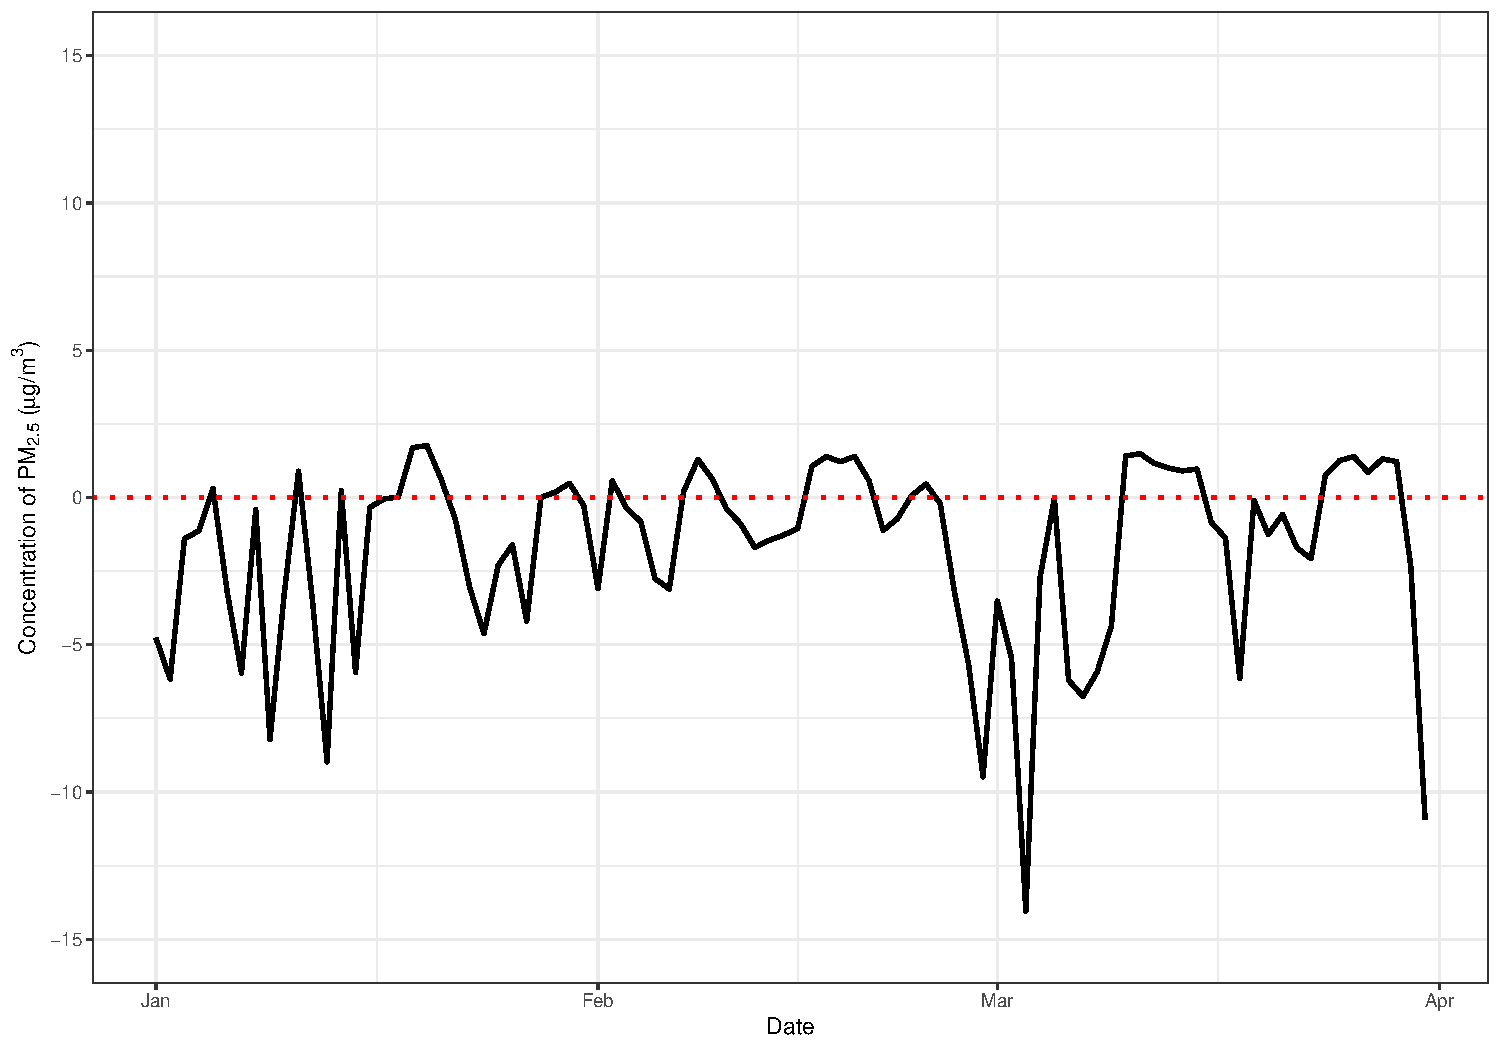
\includegraphics[width=0.85\linewidth]{Figures/Fig2b_diff}		
	\caption{Differences between daily estimated personal exposures to PM$_{2.5}$ with modelled ambient concentrations (from EMEP), see text for details). Results are presented for January - March 2021. The dotted red line denotes a difference of zero between the two series of data. } \label{fig::Fig2b_diff}
\end{figure}

\begin{figure}[!hbtp]
	\centering
	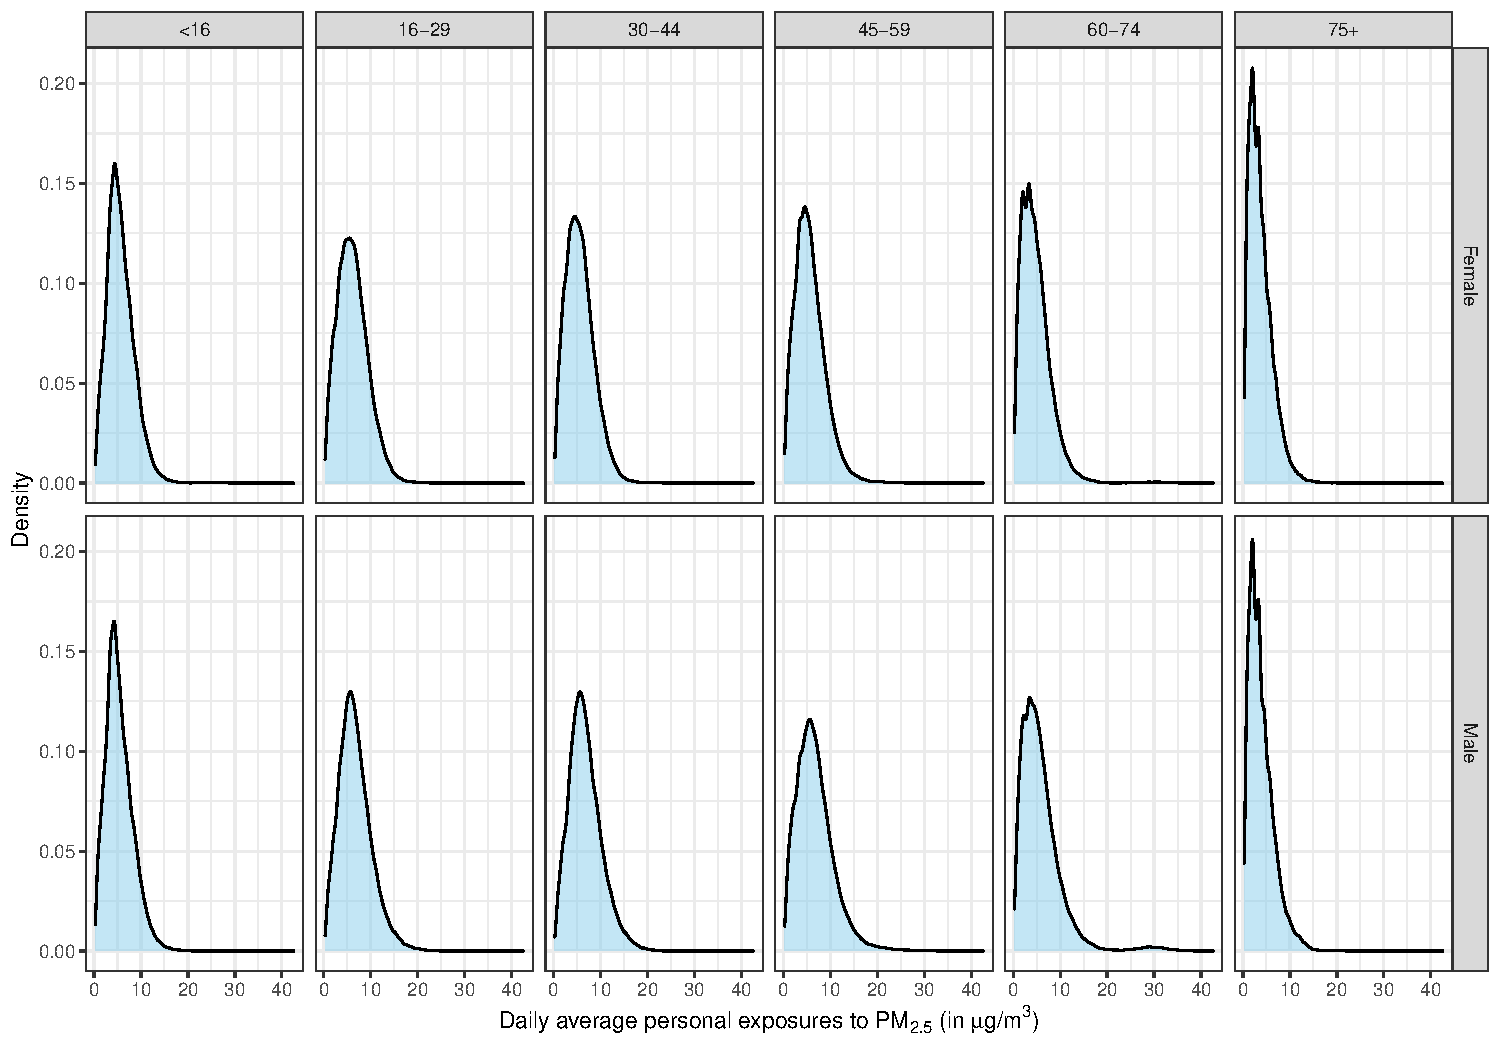
\includegraphics[width=0.72\linewidth]{Figures/Fig4a_AgeGr_Sex}		
	\caption{Distribution of daily estimated personal exposures to PM$_{2.5}$ from sampled individuals within the Manchester study area for July 2021, by age and gender. In this example, DIMEX to produce estimate personal exposures using measurements of ambient concentrations, see text for details. } \label{fig::Fig4a_AgeGr_Sex}
\end{figure}


\begin{figure}[!hbtp]
	\centering
	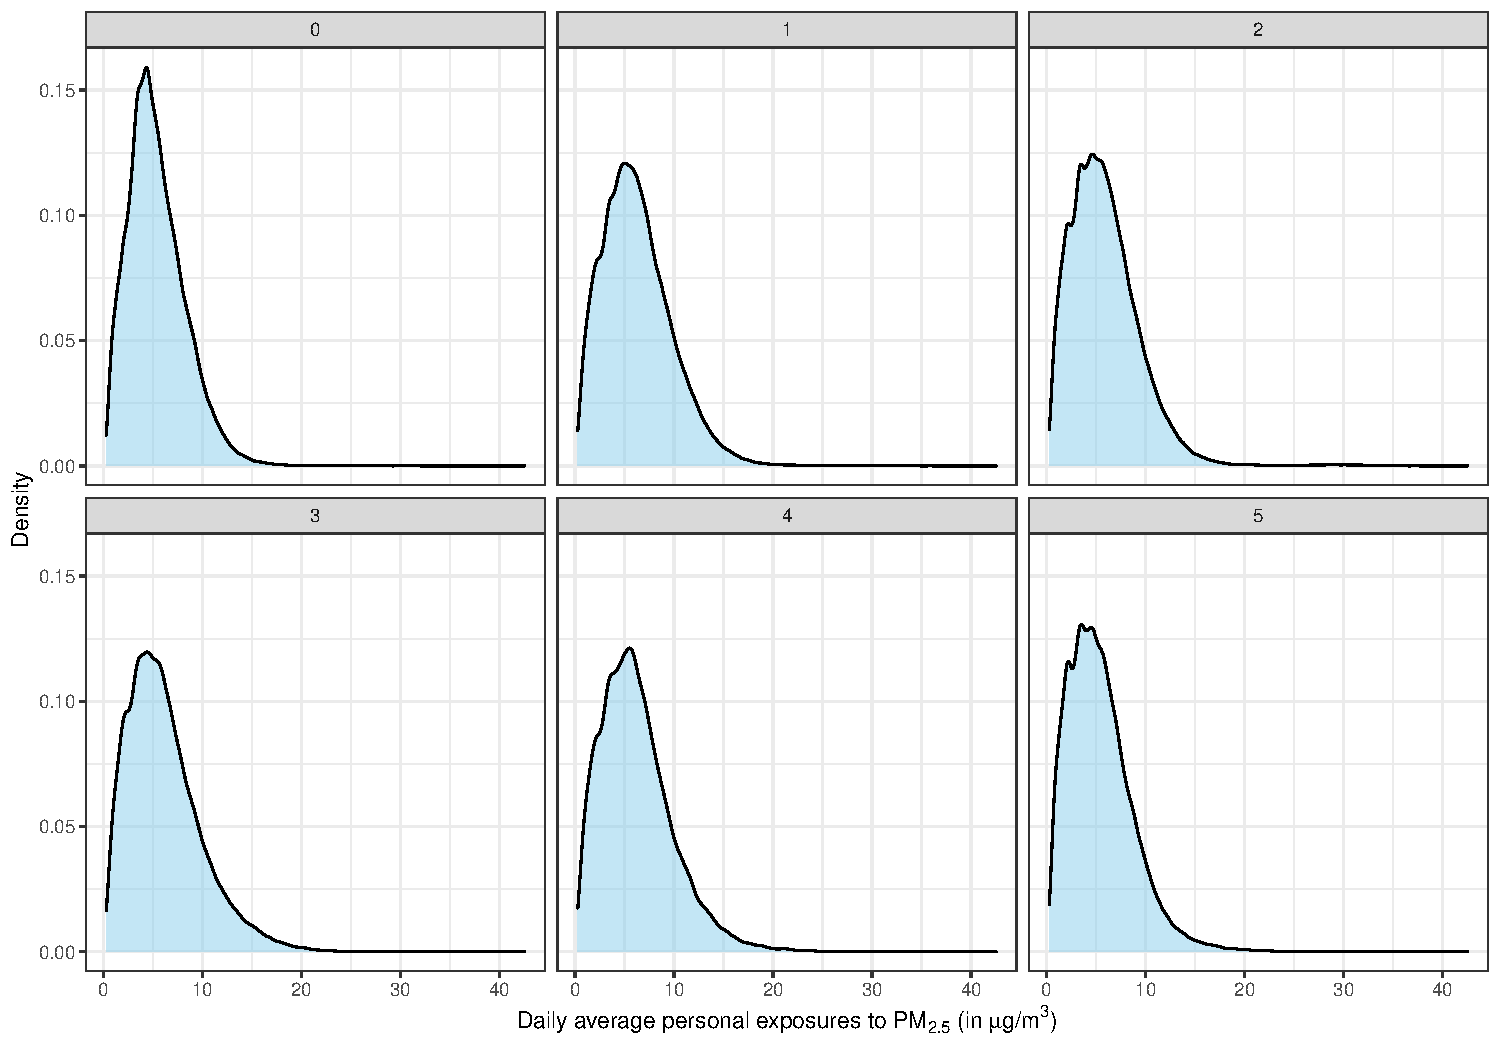
\includegraphics[width=0.72\linewidth]{Figures/Fig4a_nssec5}		
	\caption{Distribution of daily estimated personal exposures to PM$_{2.5}$ from sampled individuals within the Manchester study area for July 2021, by NSSEC socio-economic classification (0 = Not applicable/Economically inactive, 1 = Higher managerial, administrative and professional occupations, 2 = Intermediate occupations, 3 = Small employers and own account workers, 4 = Lower supervisory and technical occupations, 5 = Semi-routine and routine occupations). In this example, DIMEX to produce estimate personal exposures using measurements of ambient concentrations, see text for details. } \label{fig::Fig4a_nssec5}
\end{figure}

\begin{figure}[!hbtp]
	\centering
	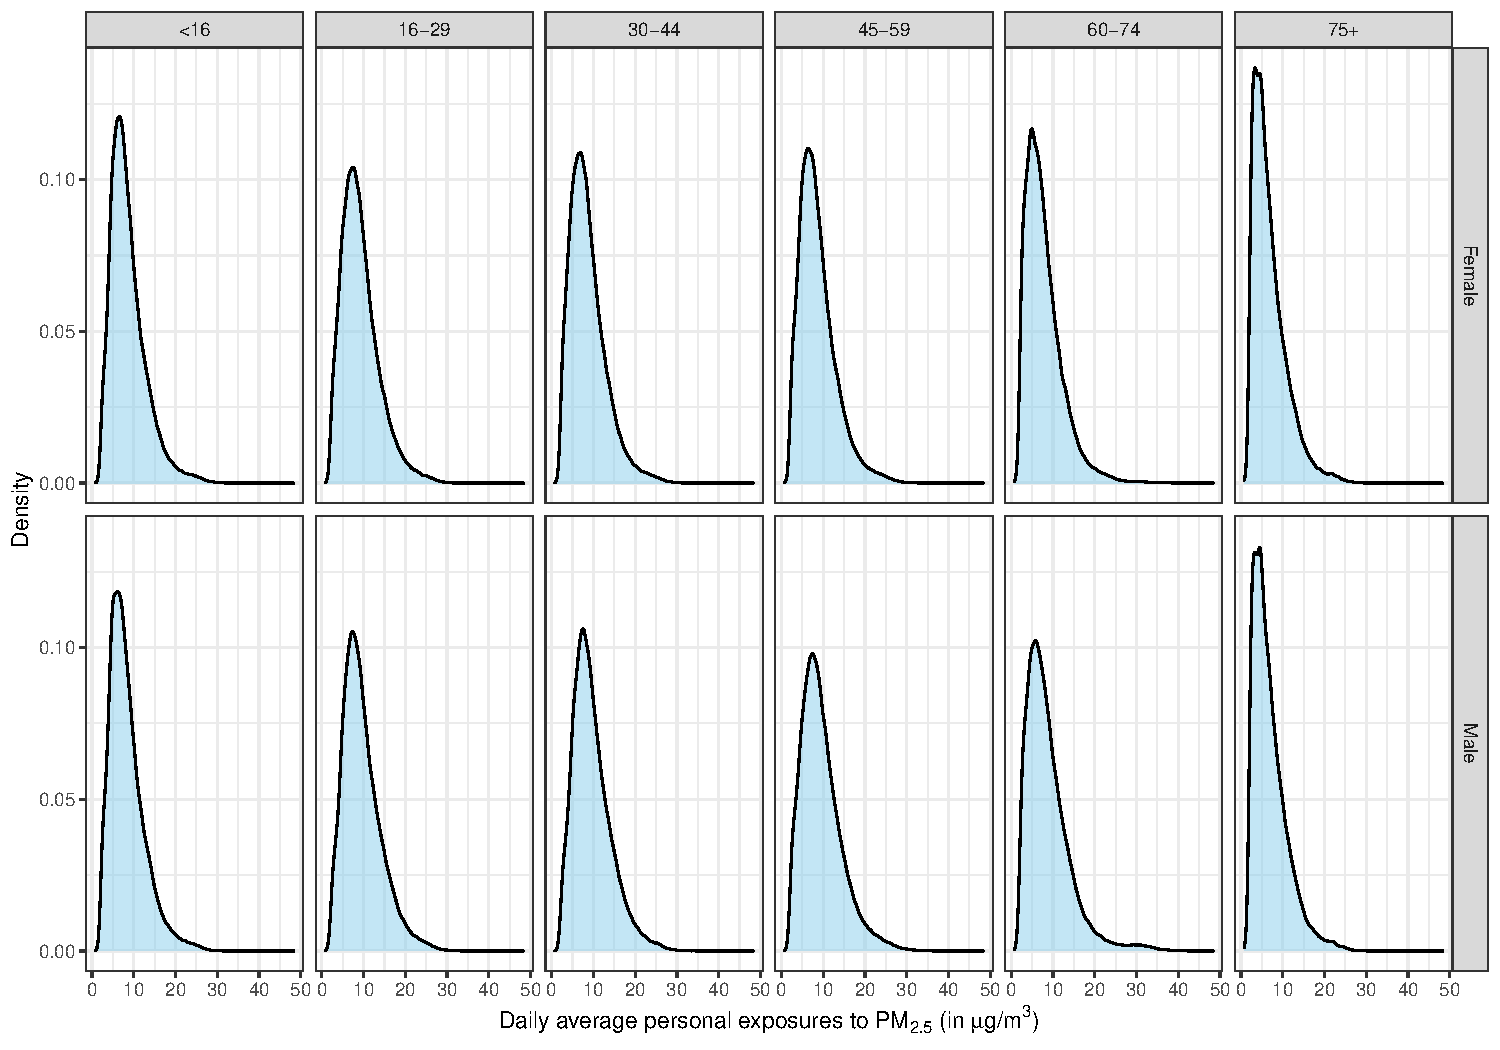
\includegraphics[width=0.72\linewidth]{Figures/Fig4b_AgeGr_Sex}		
	\caption{Distribution of daily estimated personal exposures to PM$_{2.5}$ from sampled individuals within the Manchester study area for July 2021, by age and gender. In this example, DIMEX to produce estimate personal exposures using modelled ambient concentrations, see text for details. } \label{fig::Fig4b_AgeGr_Sex}
\end{figure}

\begin{figure}[!hbtp]
	\centering
	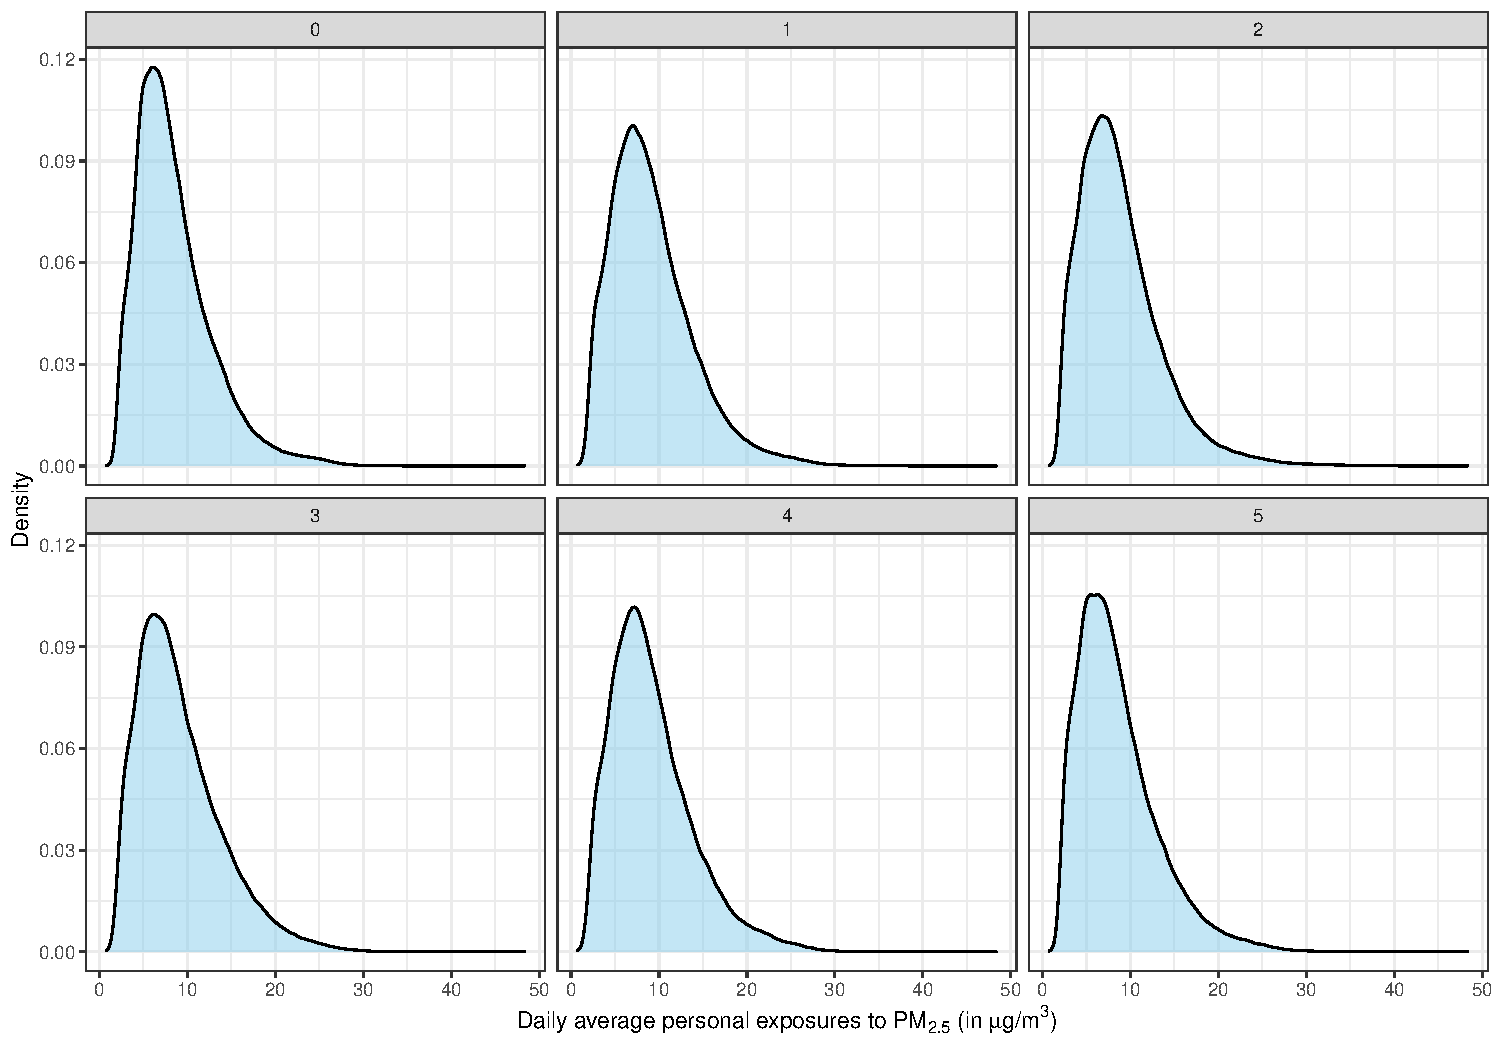
\includegraphics[width=0.72\linewidth]{Figures/Fig4b_nssec5}		
	\caption{Distribution of daily estimated personal exposures to PM$_{2.5}$ from sampled individuals within the Manchester study area for July 2021, by NSSEC socio-economic classification (0 = Not applicable/Economically inactive, 1 = Higher managerial, administrative and professional occupations, 2 = Intermediate occupations, 3 = Small employers and own account workers, 4 = Lower supervisory and technical occupations, 5 = Semi-routine and routine occupations). In this example, DIMEX to produce estimate personal exposures using modelled ambient concentrations, see text for details. } \label{fig::Fig4b_nssec5}
\end{figure}

\begin{figure}[!hbtp]
	\centering
	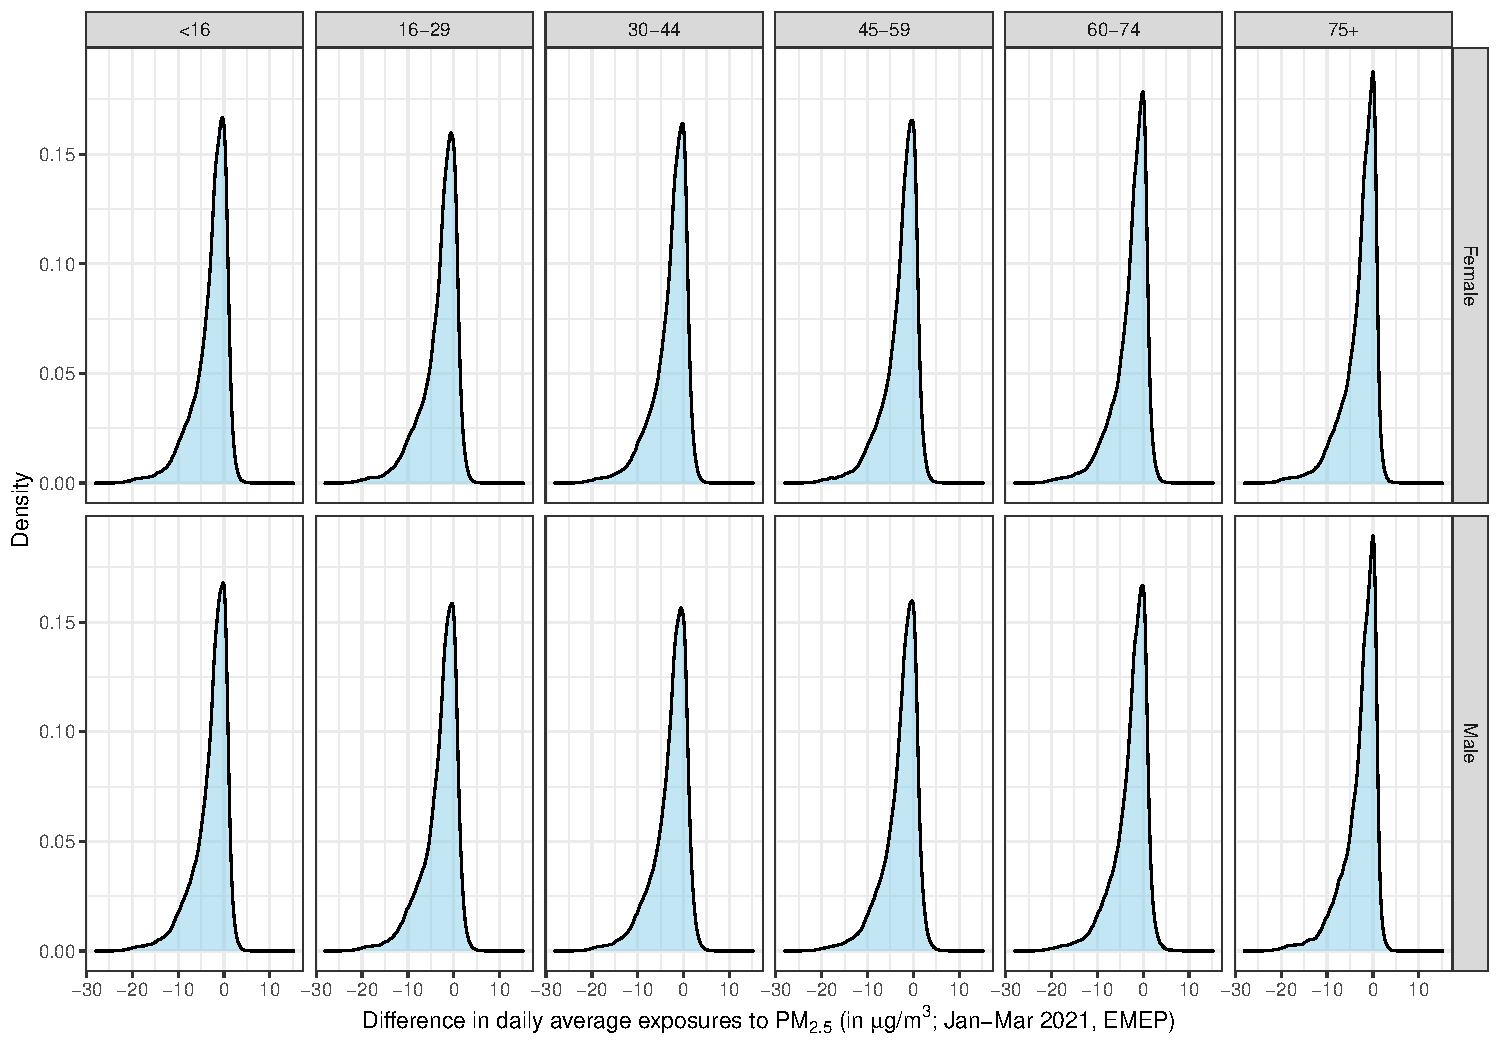
\includegraphics[width=0.9\linewidth]{Figures/Fig5b_AgeGr_Sex}		
	\caption{Distribution of differences between estimated personal exposures using modelled ambient concentrations and with ambient concentrations set to the WHO air quality guideline of 5 $\mu$g/m$^{3}$, by age and gender. Results are shown for January to March  2021 } \label{fig::Fig5b_AgeGr_Sex}
\end{figure}

\newpage 

%%%%%%%%%%%%%%%%%%%%%%%%%%%%%%%%%%%%%%%%%%%%%%%%%%%%%%%%%%%%%%%%%%
%%%%%%%%%%%%%%%%%%%%%%%%%%%%%%%%%%%%%%%%%%%%%%%%%%%%%%%%%%%%%%%%%%
%%%%%%%%%%%%%%%%%%%%%%%%%%%%%%%%%%%%%%%%%%%%%%%%%%%%%%%%%%%%%%%%%%
\clearpage
\section{Future Extensions}\label{sec::discussion}

%%%%%%%%%%%%%%%%%%%%%%%%%%%%%%%%%%%%%%%%%%%%%%%%%%%%%%%%%%%%%%%%%%
%%%%%%%%%%%%%%%%%%%%%%%%%%%%%%%%%%%%%%%%%%%%%%%%%%%%%%%%%%%%%%%%%%
%%%%%%%%%%%%%%%%%%%%%%%%%%%%%%%%%%%%%%%%%%%%%%%%%%%%%%%%%%%%%%%%%%

\noindent The DIMEX framework, using agent-based modelling to identify variations in exposures based on the movement of individuals through different micro-environments is general and can be readily applied to different pollutants, and different environmental hazards.  DIMEX-UK estimates indoor air pollution as a combination of indoor sources and the transfer of ambient pollution, based on prior knowledge and from other studies. As shown in the results from the UK Time Activity Survey and in both case studies, most people spend the vast majority of their time indoors. Indoor air quality is clearly an important area of focus and  incorporating  additional measurements on indoor micro-environments within DIMEX can be done in a straightforward fashion. \\

\noindent There is also the potential to link DIMEX with real-time measurements of air pollution and, further, to integrate it with the forecasting of concentrations ahead of time. In this Section we discuss a number of potential developments of the DIMEX framework. 

%%%%%%%%%%%%%%%%%%%%%%%%%%%%%%%%%%%%%%%%%%%%%%%%%%%%%%%%%%%%%%%%%%
%%%%%%%%%%%%%%%%%%%%%%%%%%%%%%%%%%%%%%%%%%%%%%%%%%%%%%%%%%%%%%%%%%
\clearpage
\subsection{Other pollutants, and other hazards }

%%%%%%%%%%%%%%%%%%%%%%%%%%%%%%%%%%%%%%%%%%%%%%%%%%%%%%%%%%%%%%%%%%
%%%%%%%%%%%%%%%%%%%%%%%%%%%%%%%%%%%%%%%%%%%%%%%%%%%%%%%%%%%%%%%%%%

\noindent An example of additional pollutants that could be incorporated into the DIMEX framework is exposures to biological aerosols including pollen, fungal spores and bacteria that are ubiquitous in the built up environment and they can often be allergenic, impacting the quality of life for a significant, and growing, proportion of the population. The UK has one of the highest global rates of diagnosed asthma, affecting around 10\% of adults; of the 5.3 million asthmatics in the UK someone suffers a potentially fatal asthma attack every 10 seconds, with over 1400 fatalities recorded each year. The cost to the NHS of treating allergies is around £1 billion per annum and approximately £7 billion is lost from the UK economy due to diminished productivity arising from allergies. 150 million people in the EU suffer from chronic allergenic diseases and by 2025 it is thought that over half the population will be affected, impairing quality of life and productivity.\\

\noindent The Manchester Urban Observatory (MUO) has recently acquired a state of the art Swisens Poleno realtime biological aerosol spectrometer which has now been deployed at the Fallowfield Manchester Environmental Research Institute air quality supersite for routine monitoring. The Poleno utilises holography and biofluorescence measurements to identify species via predictive machine learning pathways. The Poleno will provide researchers with speciated atmospheric concentrations of bioaerosols, initially focusing on pollen, with fungal identification capability soon to follow. This will allow us to improve our understanding of local bioaerosol emissions and sources, illuminating their impacts on air quality and human health. The UK’s first realtime pollen concentrations as derived from the Poleno are now emerging from the supersite.\\

\begin{figure}
	\centering
	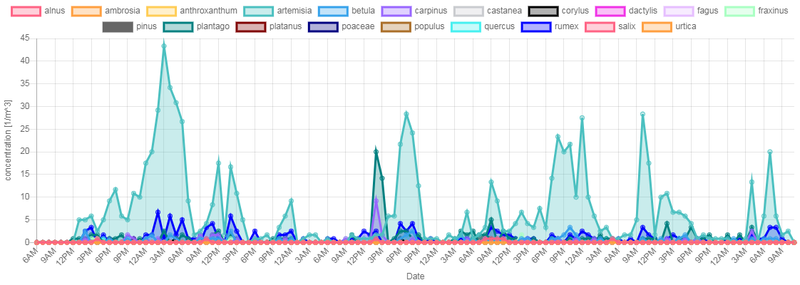
\includegraphics[width=0.95\linewidth]{Figures/poleno_firs.width-800.png}
	\caption{Real-time detection of pollen} \label{fig::pollen}
\end{figure}

\noindent The framework is also readily adaptable to other, non-pollutant bases, hazards, for example heat. An on-going example builds upon the current framework  to assess the interactions between urban environments, climate change, health and inequalities. The aim is to address the effects of projected increases in urban heat, and determine the different consequences for different population groups, e.g. for some opening a window might not be a solution due to noise or crime; how does access to green space affect health and well-being; how will different occupations be able to adapt to environmental hazards (heat, air pollution etc); what behavioural changes are possible in adapting to major events (pandemics, climate change, extreme weather etc). Similar to the situation with air quality addressed in DIMEX-UK, estimating the risks associated with higher temperatures in epidemiological studies and exposures used in health impact analyses are almost exclusively based on aggregate measures of heat (e.g. averages of measurements in an urban area or of model outputs) with the assumption that all members of the population experience the same temperatures. In reality, different members of the population will spend different amounts of time in different locations, i.e. outdoors and indoors in different types of building stock.

%%%%%%%%%%%%%%%%%%%%%%%%%%%%%%%%%%%%%%%%%%%%%%%%%%%%%%%%%%%%%%%%%%
%%%%%%%%%%%%%%%%%%%%%%%%%%%%%%%%%%%%%%%%%%%%%%%%%%%%%%%%%%%%%%%%%%
\clearpage
\subsection{Evaluating forecasting ahead of time}

%%%%%%%%%%%%%%%%%%%%%%%%%%%%%%%%%%%%%%%%%%%%%%%%%%%%%%%%%%%%%%%%%%
%%%%%%%%%%%%%%%%%%%%%%%%%%%%%%%%%%%%%%%%%%%%%%%%%%%%%%%%%%%%%%%%%%

Time-series forecasting methods have often been used to mitigate some of the challenges associated with deploying chemical transport models at high resolution for use at local scales. This does not remove the usefulness, or importance, of the latter methods in understanding wider source contributions and fate, but offers an alternative method for utilising historical local forecasts, and perhaps adapting to locally-driven forces that are important in understanding concentration and composition change. In addition, the boom in smart cities has resulted in often substantial investments in infrastructure for capturing a large number of ancillary data, which in theory can be useful for understanding changes in air-quality and potential routes for reducing exposure. Incorporating that data into time-series forecasting could enable the aforementioned stakeholders to develop systems for evaluating a series of interventions. This also holds true for building end-to-end exposure models where DIMEX could be used to estimate changes in personal exposure ahead of time. \\

\noindent There have been a number of studies developing and evaluating the use of time-series forecasting tools for air-quality. These include recent demonstrations of Long Short-Term Memory [LSTM] methods, and new demonstrations of combining Convolutional Neural Networks (CNN) and Long Short-Term Memory (LSTM) methods applied to the PM$_{2.5}$ forecasting. The availability of machine learning and statistical methods, as delivered through common programming languages, has improved significantly over the last decade. This includes widely used package such as Scikit-Learn and Keras to name a few. From a domain scientist's perspective, having the ability to prototype and tune any new method for forecasting, without requiring extensive training in building model architectures, is a bonus.These methods are similar in nature to the weather normalisation techniques developed by and others.\\

\noindent Whilst additional to the original proposed work, we have started evaluating these tools with the aim of developing a strategy for estimating changes in personal exposure ahead of time. Our focus, initially, has been on NO$_{2}$. Whilst the outcomes for DIMEX were built around PM$_{2.5}$, the drastic changes in NO$_{2}$ during the COVID lockdown presented an unfortunate opportunity to evaluate whether we could forecast ahead of time using historical patterns alone.\\

\noindent Prophet is a procedure for forecasting time series data based on an additive model where non-linear trends are fit with yearly, weekly, and daily periodicity. Developed for Facebook (now Meta), it has found applications across various domains, not least driven by the underlying rationale to develop a modular regression model with interpretive parameters that can be intuitively adjusted by analysts with domain knowledge about the time series. Our focus was on one site, Manchester Piccadilly. We refrain from performing a detailed sensitivity study of these parameters across all sites for a number of reasons, not least the local knowledge that might be needed to interpret significant interventions across regional authorities that should arise through detected change-points. Prophet relies on time-series data with clear seasonal patterns. Pollution data can exhibit strong changes through shifts in meteorological conditions that may be abnormal for a particular time of year. The standard approach for weather normalisation methods remove meteorological swings by fitting a forest based method to predict NO$_{2}$ under a range of conditions, but keeping the time axis fixed. In essence, you fit a model to hourly data over 4 years, where one of your variables is time since 1st Jan 1975 [epoch time], and then use that model to predict the concentrations at a given point in time over 10'000 met conditions but keep the epoch time as it should be. The idea is that this epoch time represents the trend term. The problem with this approach is that, whilst you get a trend line so you can look at impacts of interventions, it removes all the seasonality in the data.  In this study, we wondered  if it could be retained. If it could, then you can use Prophet to not only forecast more accurately, but also use its ability to extract change points. In figure \ref{fig::NO2normalised} we normalise by weather from the same time of day +/- 2 weeks for all years instead. You can see from the plot how we are able to retain the seasonal behaviour [orange line versus blue].\\


\begin{figure}
	\centering
	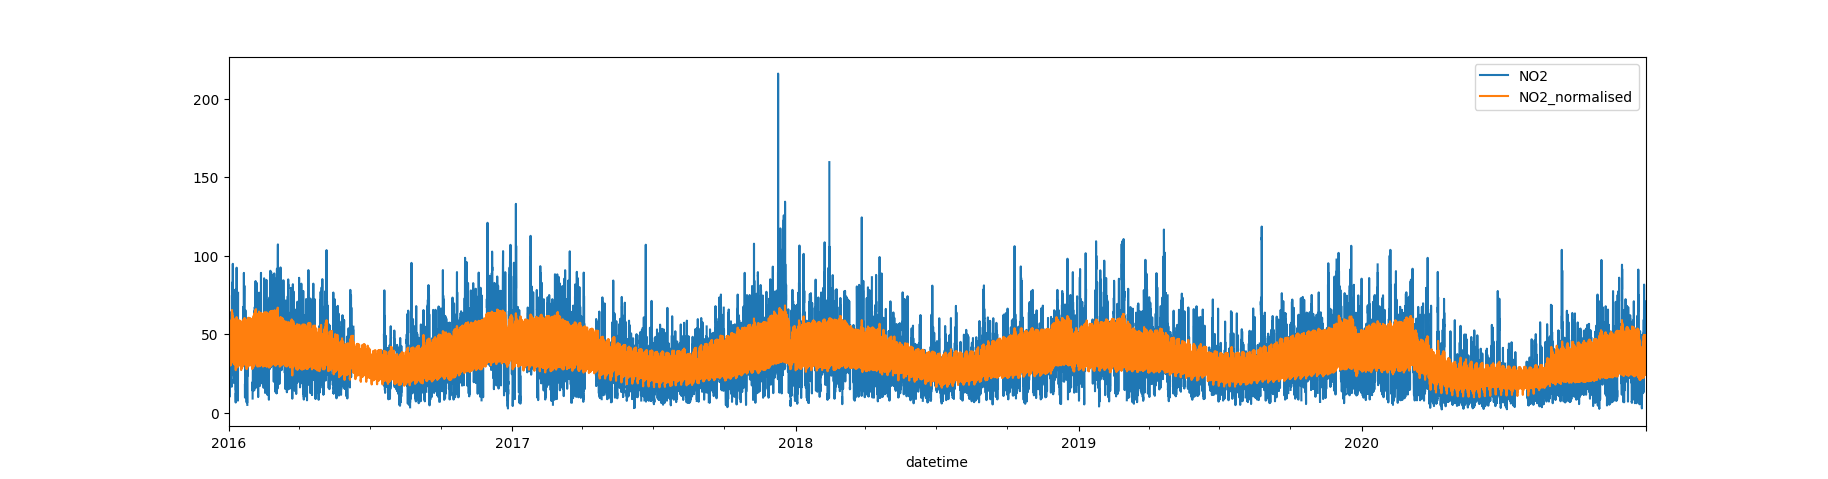
\includegraphics[width=0.95\linewidth]{Figures/NO2_raw_v_weathernorm.png}		
	\caption{'raw' versus weather normalised NO$_{2}$ before and during the first COVID lockdown. } \label{fig::NO2normalised}
\end{figure}

\noindent Please also note the period around March 2020 which represents the first lockdown period and reductions in NO$_{2}$, though still highlighting periods of high concentrations under easterly flows. This is better highlighted in Figure \ref{fig::NO2normalised2}\\

\begin{figure}[htbp]
	\centering
	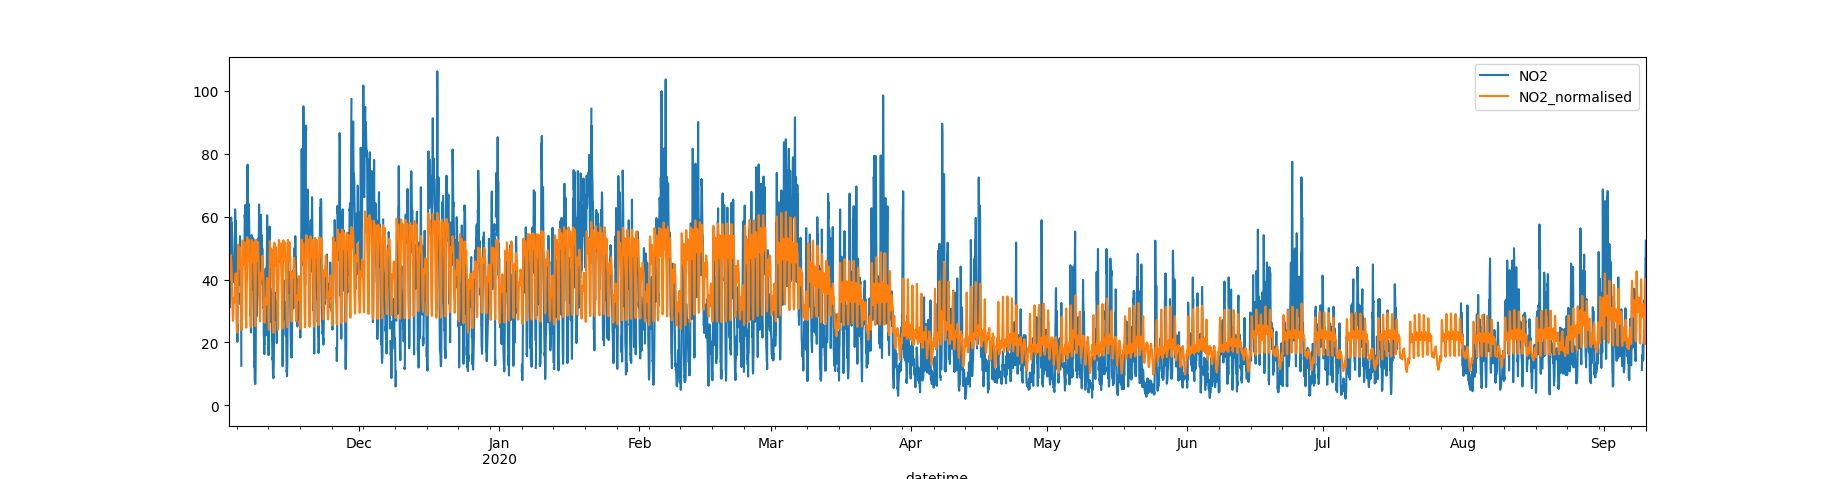
\includegraphics[width=0.95\linewidth]{Figures/NO2_raw_v_weathernorm_zoom.png}		
	\caption{'raw' versus weather normalised NO$_{2}$ before and during the first COVID lockdown (zoomed in). } \label{fig::NO2normalised2}
\end{figure}

\noindent More importantly, with this new normalised data, Prophet is able to capture the drastic changes very well, using the past 72 hours to forecast 3 hours in advance, even without any traffic data as extra regressor variables. This is displayed in figure \ref{fig::NO2normalised3} below. \\

\begin{figure}[htbp]
	\centering
	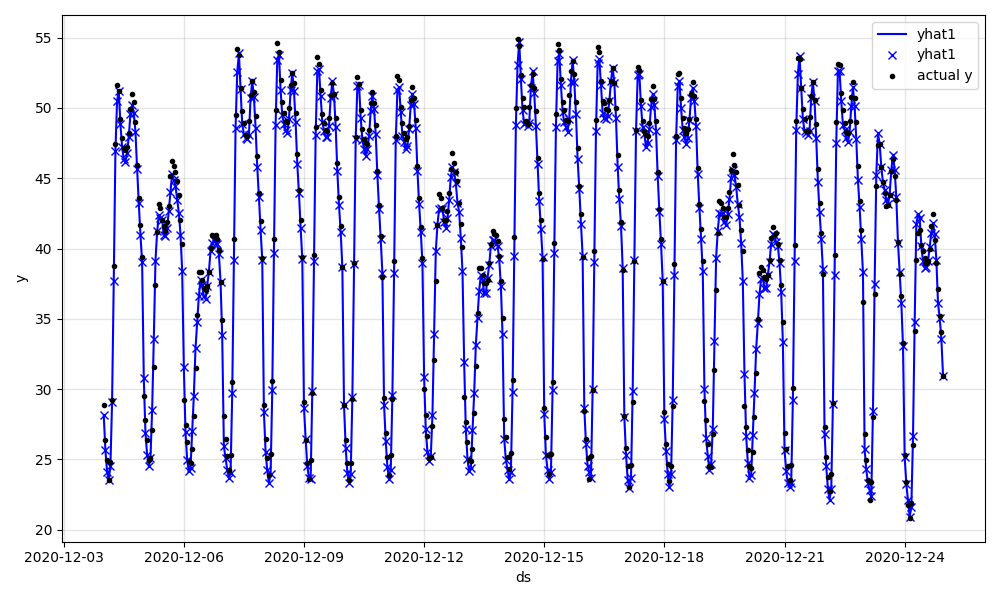
\includegraphics[width=0.95\linewidth]{Figures/forecast_1month.png}
	\caption{Measured, weather normalised, data (black dots) compared with forecast values (blue)} \label{fig::NO2normalised3}
\end{figure}

\noindent Moreover, we then have the ability to then pick out change-points, including the influence of national holidays etc as per figure \ref{fig::changepoints}.\\

\begin{figure*}[htbp]
	\centering
	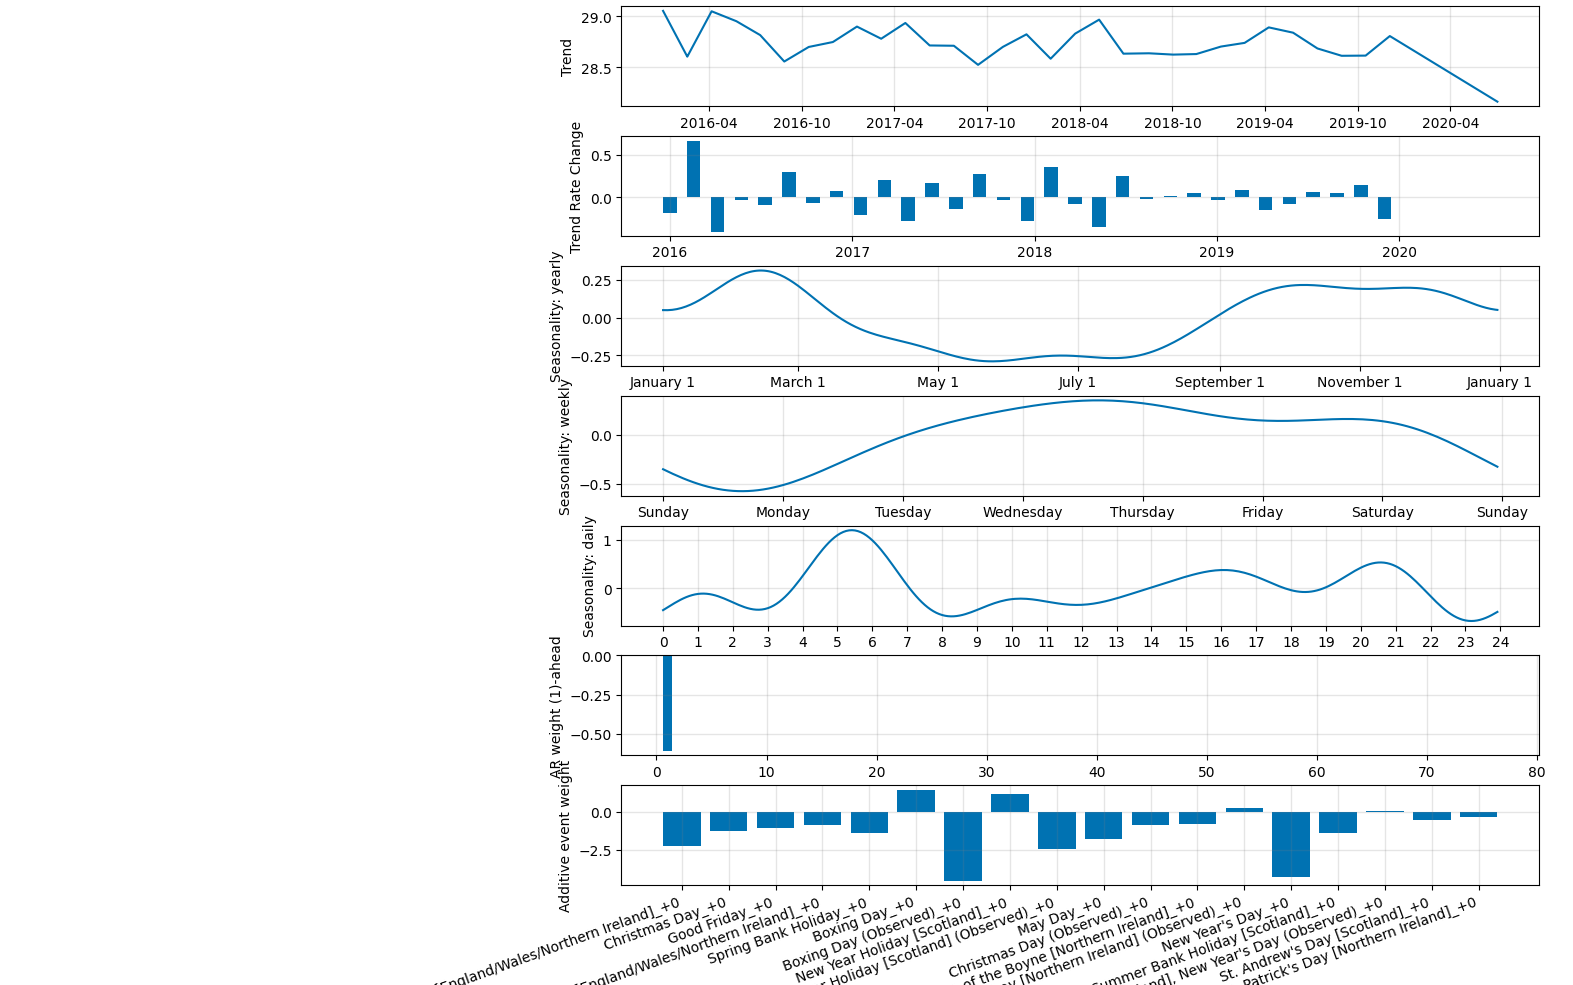
\includegraphics[width=0.95\linewidth]{Figures/components.png}		
	\caption{Extracted change-points and trend terms to better understand potential changes in personal exposure and links to emission/source profiles} \label{fig::changepoints}
\end{figure*}

\noindent This work is very much in its infancy; however it does create a path for ongoing investigations around forecasting ahead of time. Expanding this work to PM$_{2.5}$ will require careful consideration around the lack of seasonality in PM$_{2.5}$ trends. This, coupled with different atmospheric factors, will likely require integration of methods such as LSTMs and CNN approaches that account for land-use. Nonetheless, in targeting changes in energy infrastructure and the uncertain contribution of a hydrogen economy, this method shows potential for further development of DIMEX into the development of Digital Twins.

%%%%%%%%%%%%%%%%%%%%%%%%%%%%%%%%%%%%%%%%%%%%%%%%%%%%%%%%%%%%%%%%%%
%%%%%%%%%%%%%%%%%%%%%%%%%%%%%%%%%%%%%%%%%%%%%%%%%%%%%%%%%%%%%%%%%%
\clearpage
\subsection{Creating spatially enriched synthetic micro-data for national multi-level modelling}

%%%%%%%%%%%%%%%%%%%%%%%%%%%%%%%%%%%%%%%%%%%%%%%%%%%%%%%%%%%%%%%%%%
%%%%%%%%%%%%%%%%%%%%%%%%%%%%%%%%%%%%%%%%%%%%%%%%%%%%%%%%%%%%%%%%%%

Spatial microsimulation, whether defined as a method or approach \citep{LovelaceR.Dumont2016}, is nowadays a well-known technique for integration of census data and detailed surveys with a wide variety of applications, mainly to help analyse policy strategies \citep{Hermes2012,Tanton2013,tanton2018spatial,Spiekermann2018}. With new methodological developments, calibration metrics and integration of new survey data, more microsimulation use cases are being presented worldwide. This technique provides models like DIMEX, the synthetic data required to analyse time-sensitive but, more importantly, national-scale issues in areas like public health, climate change or transportation that may have quite different impacts across different local communities.\\

\noindent In this context, spatial microsimulation offers a way to parametrise or add new levels of complexity to existing models by providing synthetic data with multiple dimensions. Despite the latest progress in this approach, its applications remain to be developed further. Along with the extensive computational requirements, there is an excessive and inherent complexity in the integration of multiple data sources; therefore, creating consistent synthetic datasets from sources with different spatial and temporal resolutions is a persistent challenge that has typically been addressed for a limited area \citep{Tanton2017}. \\

\noindent \cite{Spiekermann2018} presents a vision that emphasises that with enough complexity incorporated into the model, researchers should not lose their focus and model what is indeed required. The challenge is, therefore, to find out the balance between complexity and the description of a given issue, keeping the model as complex as strictly necessary, bearing in mind what needs to be done rather than what can be done. Unfortunately, there is a lack of reproducibility, reusability and indeed a shortage of tools and methods that create significant barriers for researchers that require synthetic populations easily integrated with other models. Overall, the most complicated and time-consuming part of the multi-level modelling process does not rely upon the topic to model, but the synthetic population required. \\

\noindent As part of a major programme to develop and demonstrate the importance of AI and data science for government and planning systems, the Alan Turing Institute has established multiple research programs to exploit the power of behavioural modelling and spatial analysis to increase the robustness of social systems \citep{UA_ATI}, researchers have sought to develop new tools to contribute to the simplification of the process of generating synthetic population datasets. Built upon previous efforts like \citep{spooner2021dynamic}; a new tool has been initially deployed. The Synthetic Population Catalyst or SPC \citep{Carlino2022} is a tool that incorporates the spatial microsimulation model from (SPENSER) combined with the United Kingdom Time Use Survey (UKTUS) and the Health Survey of England (HSE). The spatial integration and transportation model – QUANT to model the trips to schools and retail, model of commuting flows, and salaries (hourly and annually) from the Office for National Statistics (ONS) salary data.\\

\noindent The SPC tool generates synthetic population (individuals and households) datasets covering all of England (national level) at MSOA granularity for the year 2020. There are two ways users can take advantage of this tool; initially, users can explore, reuse, and understand how the output file is structured by downloading any of the ceremonial counties in England (officially called lieutenancy areas). Otherwise, users can generate their own area by installing and executing the tool in their environment. SPC requires a list of MSOAs. The model will fetch the corresponding data and assemble them into protocol buffer files that encapsulate all the requested information for a given area. A schematic of this process can be seen in  Figure \ref{fig:SPC}.\\


\begin{figure}[h]
\centering
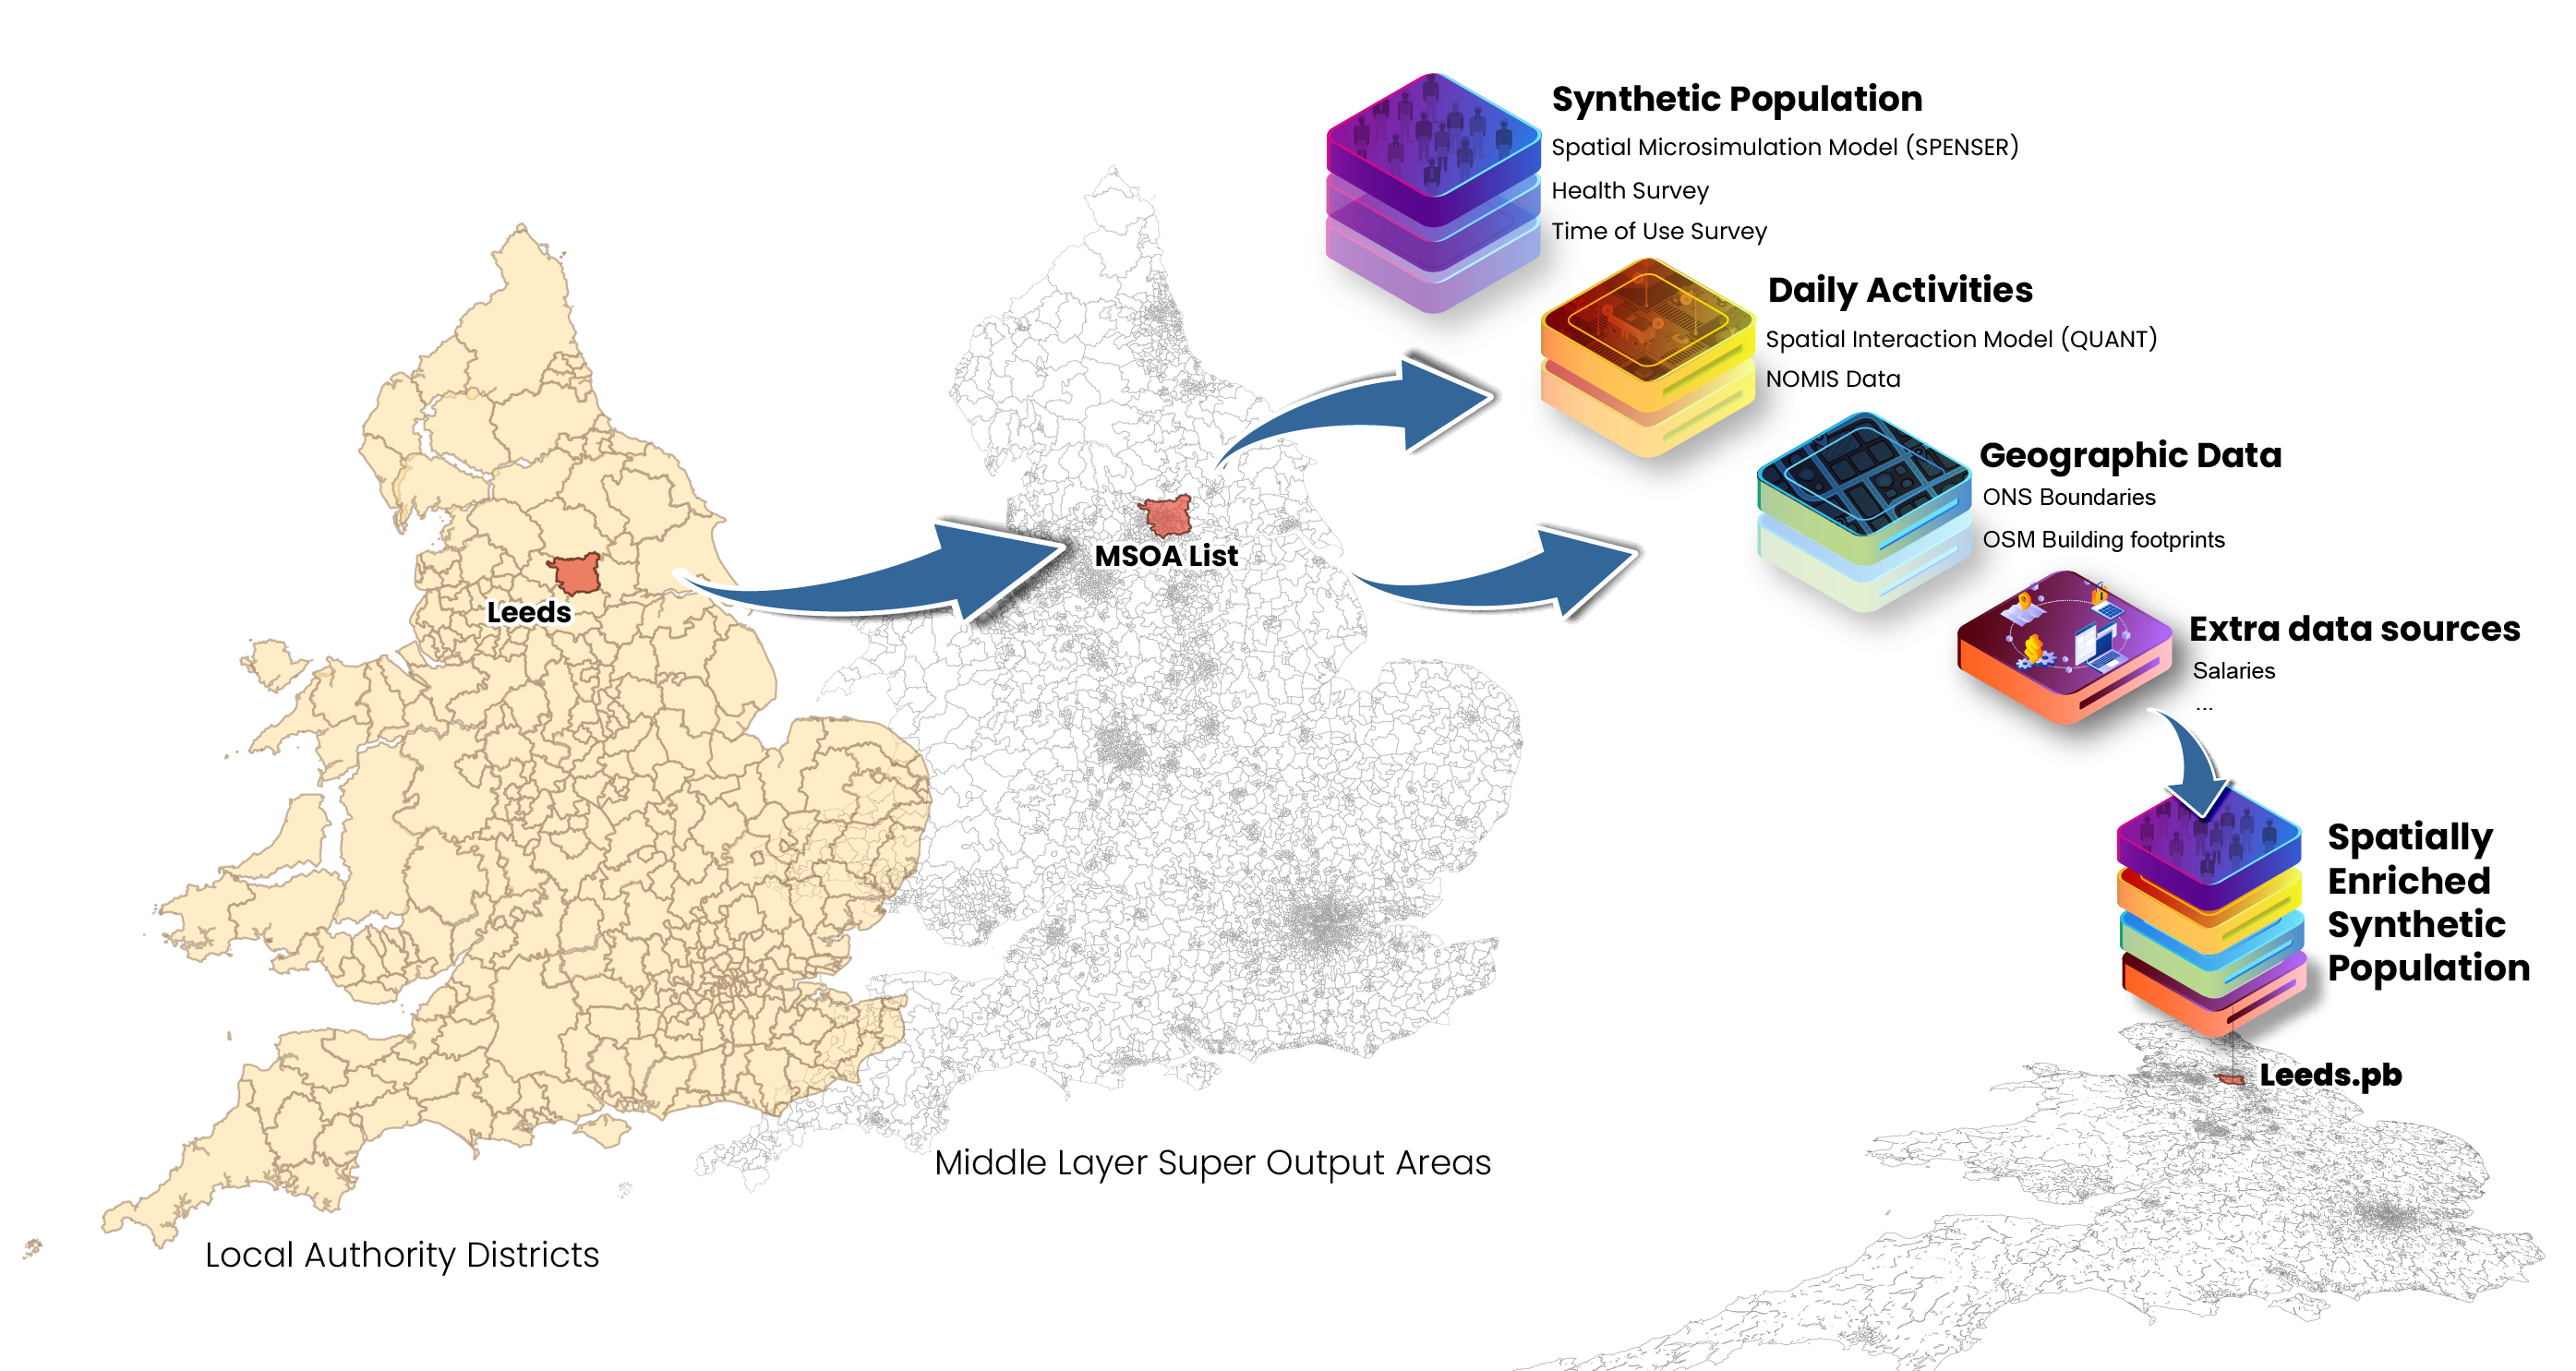
\includegraphics[width = \textwidth]{Figures/SPC_Schema.png}
\caption{Schematic of the Synthetic Population Catalyst process }\label{fig:SPC}
\end{figure}



\noindent By providing the data product and tool in a reproducible environment \citep{CarlinoRepo}, users can explore and integrate the synthetic population dataset in their external models and not deal with the complicated and time-consuming installation processes. The data schema integrated into the tool is publicly available in \citep{CarlinoRepo} as well as the code where more collaboration is welcome. In case the users have the technical skills to install the tool and require a synthetic population for a custom area, the tool includes a set of scripts to guide them to quickly get the list of MSOAs by defining the name of the desired Local Authority or LAD. \\

\noindent Despite being a work in progress, the SPC tool has already identified use cases that can initially provide synthetic population files to model topics beyond the originally conceived COVID modelling approach. Areas like climate change and its impact, the DIMEX model, or the study of social inequalities can benefit from having a scalable, central, easy to use and computationally efficient tool to address the initial step of any urban modelling process, the creation of spatially enriched synthetic microdata.

%%%%%%%%%%%%%%%%%%%%%%%%%%%%%%%%%%%%%%%%%%%%%%%%%%%%%%%%%%%%%%%%%%
%%%%%%%%%%%%%%%%%%%%%%%%%%%%%%%%%%%%%%%%%%%%%%%%%%%%%%%%%%%%%%%%%%


%%%%%%%%%%%%%%%%%%%%%%%%%%%%%%%%%%%%%%%%%%%%%%%%%%%%%%%%%%%%%%%%%%
%%%%%%%%%%%%%%%%%%%%%%%%%%%%%%%%%%%%%%%%%%%%%%%%%%%%%%%%%%%%%%%%%%
%%%%%%%%%%%%%%%%%%%%%%%%%%%%%%%%%%%%%%%%%%%%%%%%%%%%%%%%%%%%%%%%%%

\newpage 
\bibliographystyle{mattnat}
\bibliography{refs}
\newpage 

%%%%%%%%%%%%%%%%%%%%%%%%%%%%%%%%%%%%%%%%%%%%%%%%%%%%%%%%%%%%%%%%%%
%%%%%%%%%%%%%%%%%%%%%%%%%%%%%%%%%%%%%%%%%%%%%%%%%%%%%%%%%%%%%%%%%%
%%%%%%%%%%%%%%%%%%%%%%%%%%%%%%%%%%%%%%%%%%%%%%%%%%%%%%%%%%%%%%%%%%

\begin{appendix}

%%%%%%%%%%%%%%%%%%%%%%%%%%%%%%%%%%%%%%%%%%%%%%%%%%%%%%%%%%%%%%%%%%
%%%%%%%%%%%%%%%%%%%%%%%%%%%%%%%%%%%%%%%%%%%%%%%%%%%%%%%%%%%%%%%%%%
%%%%%%%%%%%%%%%%%%%%%%%%%%%%%%%%%%%%%%%%%%%%%%%%%%%%%%%%%%%%%%%%%%

% Resetting figure and table count for the appendix
\setcounter{figure}{0} \renewcommand{\thefigure}{A.\arabic{figure}}
\setcounter{table}{0} \renewcommand{\thetable}{A.\arabic{table}}

%%%%%%%%%%%%%%%%%%%%%%%%%%%%%%%%%%%%%%%%%%%%%%%%%%%%%%%%%%%%%%%%%%
%%%%%%%%%%%%%%%%%%%%%%%%%%%%%%%%%%%%%%%%%%%%%%%%%%%%%%%%%%%%%%%%%%
%%%%%%%%%%%%%%%%%%%%%%%%%%%%%%%%%%%%%%%%%%%%%%%%%%%%%%%%%%%%%%%%%%
\clearpage
\section{Appendix}

%%%%%%%%%%%%%%%%%%%%%%%%%%%%%%%%%%%%%%%%%%%%%%%%%%%%%%%%%%%%%%%%%%
%%%%%%%%%%%%%%%%%%%%%%%%%%%%%%%%%%%%%%%%%%%%%%%%%%%%%%%%%%%%%%%%%%
%%%%%%%%%%%%%%%%%%%%%%%%%%%%%%%%%%%%%%%%%%%%%%%%%%%%%%%%%%%%%%%%%%

\renewcommand{\arraystretch}{1.5}

\begin{table}[H]
%	\footnotesize
	\centering
	\caption{Prior distributions of the model parameters estimating concentrations of PM$_{2.5}$ in open micro-environments.}
	\begin{tabular}{l l l l l}
		\hline \hline 
		Micro-environment ($m$) & Intercept ($a_m$) & Slope ($b_m$) & Variability of local & Source \\
		\hline 
		Outdoor                 & 0               & 1           & -                     & \citet{zidek2007framework} \\ 
		Indoor not home         & $N$(6.467, 2.1) & $N$(0.507, 0.11) & N(local, 3.467) & \citet{burke2001population} \\
		Transport               & $N$(33, 7.2)    & $N$(0.26, 0.14) &  N(local, 12) & \citet{burke2001population} \\
		\hline \hline 
	\end{tabular}
	\label{tab::openmicro}
\end{table}

\begin{table}[H]
	\footnotesize
	\centering
	\caption{Prior distributions of the model parameters estimating concentrations of PM$_{2.5}$ in the `home' micro-environment.}
	\begin{tabular}{l l l l}
		\hline \hline 
		Parameter & Setting & Value & Source \\
		\hline 
		$S_t$                       & Cooking                      & N(1.7, 0.325)       & \citet{ozkaynak1996personal} \\
		                             & Smoking                      & N(13.8, 1.775)      & \citet{ozkaynak1996personal} \\
		                             & Other                        & N(1.1, 0.525)       & \citet{ozkaynak1996personal} \\
		$V$                          & Square footage detached      & Tri(81, 214, 159)   & Zoopla \\
		                             & Square footage semi-detached & Tri(56, 204, 84)    & Zoopla \\
		                             & Square footage terrace       & Tri(33, 155, 59)    & Zoopla \\
		                             & Square footage flat          & Tri(34, 106, 41)    & Zoopla \\
		                             & Ceiling height               & Unif(2.1, 2.6)      & Zoopla \\
		$v$                          & Winter                       & logN(-0.957, 0.589) & \citet{murray1995residential} \\
		                             & Spring                       & logN(-0.802, 0.782) & \citet{murray1995residential} \\
		                             & Summer                       & logN(-0.583, 0.612) & \citet{murray1995residential} \\
		                             & Autumn                       & logN(-0.787, 0.453) & \citet{murray1995residential} \\
		$F^p$                        &                              & N(1, 0.055)         &  \citet{burke2001population}\\
		$F^d$                        &                              & N(0.39, 0.0825)     &  \citet{burke2001population}\\
		Hourly Cigarette Consumption & Female, 16-24                & Pois(5/15)          & \citet{ONS2020} \\
		                             & Female, 25-34                & Pois(6.9/15)        & \citet{ONS2020} \\
		                             & Female, 35-49                & Pois(8.33/15)       & \citet{ONS2020} \\
		                             & Female, 50-59                & Pois(10.5/15)       & \citet{ONS2020} \\
		                             & Female, 60+                  & Pois(10.8/15)       & \citet{ONS2020} \\
		                             & Male, 16-24                  & Pois(4/15)          & \citet{ONS2020} \\
		                             & Male, 25-34                  & Pois(4.55/15)       & \citet{ONS2020} \\
		                             & Male, 35-49                  & Pois(8.97/15)       & \citet{ONS2020} \\
		                             & Male, 50-59                  & Pois(11.9/15)       & \citet{ONS2020} \\
		                             & Male, 60+                    & Pois(12.9/15)       & \citet{ONS2020} \\
		Concentration starting point &                              & N(26, 2)            & \citet{wallace1993indoor} \\
		\hline \hline 
	\end{tabular}
	\label{tab::closedmicro}
\end{table}

\end{appendix}
%%%%%%%%%%%%%%%%%%%%%%%%%%%%%%%%%%%%%%%%%%%%%%%%%%%%%%%%%%%%%%%%%%

\end{document}

%%%%%%%%%%%%%%%%%%%%%%%%%%%%%%%%%%%%%%%%%%%%%%%%%%%%%%%%%%%%%%%%%%















